%%%%%%%%%%%%%%%%%%%%%%%%%%%%%%%%%%%%%%%%%%%%%%%%%%%%%%%%%%%%%%%%%%%%%%%%
% This is the main file of the Msc thesis template.
%%%%%%%%%%%%%%%%%%%%%%%%%%%%%%%%%%%%%%%%%%%%%%%%%%%%%%%%%%%%%%%%%%%%%%%%
%
% Author:   René Widmer
%           Institute for Surgical Technology and Biomechanics ISTB
%           University of Bern
%           rene.widmer@istb.unibe.ch
%
% Date:     10/28/2009
%
%%%%%%%%%%%%%%%%%%%%%%%%%%%%%%%%%%%%%%%%%%%%%%%%%%%%%%%%%%%%%%%%%%%%%%%%

\pdfminorversion=6
\documentclass[a4paper,10pt,openright]{unibe-msc}
% Some regulary used packages
\usepackage{etex}
\usepackage[T1]{fontenc}
\usepackage{textcomp}
\usepackage{bm}
\usepackage[utf8]{inputenc}
\usepackage[pdftex,final]{graphicx}
\usepackage{amssymb}
\usepackage{amsmath}                    
\usepackage{amsfonts}
\usepackage{mathtools}
\usepackage{ulem}
\usepackage[english]{babel}
\usepackage{url}
\usepackage{color}
\usepackage{unibe-msc}
\usepackage[caption=off]{subfig}
\usepackage{hyperref}
\usepackage{float}


% Default graphics path
\graphicspath{{Images/}{Logos/}{images/}}

% Document metadata
\unibelogo{ub_16pt_192}  % Don't change this
\htilogo{TI_e} % Don't change this
\faculty{Faculty of Medicine} % Don't change this
\discipline{Biomedical Engineering} % Don't change this
\subtitle{Master of Science Thesis} % Don't change this
\title{3D Liver Reconstruction from Tracked Ultrasound}
\author{Luca Sahli}
\origin{Wohlen b. Bern, Switzerland}
\date{\today}
\supervisor{MSc Iwan Paolucci and Prof. Dr.-Ing. Stefan Weber}
\affiliation{ARTORG Center for Biomedical Engineering Research, University of Bern}

\examiner{Prof. Dr.-Ing. Stefan Weber and MSc Iwan Paolucci}
\place{Bern}
\frontsignature{\theplace, October 2018}
\date{October 31\textsuperscript{th} 2018}

%%%%%%%%%%%%%%%%%%%%%%%%%%%%%%%%%%%%%%%%%%%%%%%%%%%%%%%%%%%%%%%%%%%%%
% Hyperref setup
%%%%%%%%%%%%%%%%%%%%%%%%%%%%%%%%%%%%%%%%%%%%%%%%%%%%%%%%%%%%%%%%%%%%%
% Appearance of hyper links
\definecolor{lc}{rgb}{0,0,0}
\hypersetup{colorlinks=true, breaklinks=true, linkcolor=lc, 
                  menucolor=lc, urlcolor=lc, anchorcolor=lc,
                  citecolor=lc, filecolor=lc,
                  pdftitle=\thetitle,
                  pdfauthor=\theauthor,
                  pdfsubject=Master Thesis,
                  pdfkeywords={Keyword 1, Keyword 2, Keyword 3},
                  pdfpagelayout=SinglePage}
                  
% Bibliography style file
\bibliographystyle{ieee}

\begin{document}
SDFSDFSDF
%%%%%%%%%%%%%%%%%%%%%%%%%%%%%%%%%%%%%%%%%%%%%%%%%%%%%%%%%%%%%%%%%%%%%
% Titlepage, abstract table of contents etc.
%%%%%%%%%%%%%%%%%%%%%%%%%%%%%%%%%%%%%%%%%%%%%%%%%%%%%%%%%%%%%%%%%%%%%
\frontmatter
\maketitle
%%%%%%%%%%%%%%%%%%%%%%%%%%%%%%%%%%%%%%%%%%%%%%%%%%%%%%%%%%%%%%%%%%%%%%%%
% This is the conclusion chapter file.
%%%%%%%%%%%%%%%%%%%%%%%%%%%%%%%%%%%%%%%%%%%%%%%%%%%%%%%%%%%%%%%%%%%%%%%%
%
% Author:   René Widmer
%           Institute for Surgical Technology and Biomechanics ISTB
%           University of Bern
%           rene.widmer@istb.unibe.ch
%
% Date:     10/28/2009
%
%%%%%%%%%%%%%%%%%%%%%%%%%%%%%%%%%%%%%%%%%%%%%%%%%%%%%%%%%%%%%%%%%%%%%%%%

\begin{abstract}

\noindent\textit{The abstract should provide a concise (300-400 word) summary of the motivation, methodology, main results and conclusions. For example:}

\vskip1em

Osteoporosis is a disease in which the density and quality of bone are reduced. As the bones become more porous and fragile, the risk of fracture is greatly increased. The loss of bone occurs progressively, often there are no symptoms until the first fracture occurs. Nowadays as many women are dying from osteoporosis as from breast cancer. Moreover it has been estimated that yearly costs arising from osteoporotic fractures alone in Europe worth 30 billion Euros.

Percutaneous vertebroplasty is the injection of bone cement into the vertebral body in order to relieve pain and stabilize fractured and/or osteoporotic vertebrae with immediate improvement of the symptoms. Treatment risks and complications include those related to needle placement, infection, bleeding and cement extravazation. The cement can leak into extraosseous tissues, including the epidural or paravertebral venous system eventually ending in pulmonary embolism and death.

The aim of this project was to develop a computational model to simulate the flow of two immiscible fluids through porous trabecular bone in order to predict the three-dimensional spreading patterns developing from the cement injection and minimize the risk of cement extravazation while maximizing the mechanical effect. The computational model estimates region specific porosity and anisotropic permeability from Hounsfield unit values obtained from patient-specific clinical computer tomography data sets. The creeping flow through the porous matrix is governed by a modified version of Darcy's Law, an empirical relation of the pressure gradient to the flow velocity with consideration of the complex rheological properties of bone cement.

To simulate the immiscible two phase fluid flow, i.e. the displacement of a biofluid by a biomaterial, a fluid interface tracking algorithm with mixed boundary representation has been developed. The nonlinear partial differential equation arising from the problem was numerically implemented into the open-source Finite Element framework \textit{libMesh}. The algorithm design allows the incorporation of the developed methods into a larger simulation of vertebral bone augmentation for pre-surgical planning.

First simulation trials showed close agreement with the findings from relevant literature. The computational model demonstrated efficiency and numerical stability. The future model development may incorporate the morphology of the region specific trabecular bone structure improving the models' accuracy or the prediction of the orientation and alignment of fiber-reinforced bone cements in order to increase fracture-resistance. 

\end{abstract}

\endinput
%%% Local Variables:
%%% TeX-master: "MscThesis"
%%% End:
\clearpage
\chapter*{Acknowledgements}
First, I would like to thank my thesis supervisors, Iwan Paolucci and
  Prof. Dr.-Ing. Stefan Weber of the IGT group in the ARTORG Center for
  Biomedical Engineering, who supported and steered my work in the right
  direction with a lot of helpful advices.
  I would also like to thank the other
  members of the IGT group for their support during the thesis and the discussions
  during the coffee breaks. 
  A special thanks goes to the surgeons who
  participated in the phantom experiments, namely Dr. med. Pascale Tinguely, Dr.
  Gabriela Pereira Bom Braga and Dr. Catherine Tsai, MD for their valuable
  inputs and feedbacks. Another special thanks goes to Raluca Sandu and Ankit
  Gupta for their everyday support and proofreading of the thesis.
 Last but not least I would also like to thank my parents, brothers and friends for their support regardless
of the field.
\endinput
%%% Local Variables:
%%% TeX-master: "MscThesis"
%%% End:
\clearpage

\vspace*{0cm}
\vfill
\noindent\parbox[b][0.5\textheight]{\textwidth}
{
		\vfill
		\noindent\normalsize\mdseries\itshape
Ich erkläre hiermit, dass ich diese Arbeit selbständig verfasst und keine anderen als die angegebenen Hilfsmittel benutzt habe. Alle Stellen, die wörtlich oder sinngemäss aus Quellen entnommen wurden, habe ich als solche kenntlich gemacht. Mir ist bekannt, dass andernfalls der Senat gemäss dem Gesetz über die Universität zum Entzug des auf Grund dieser Arbeit verliehenen Titels berechtigt ist.\par
		\vspace{2cm}
		\noindent\normalsize\normalfont
		{
			Bern, \thedate\par
		}\par
		\vspace{2cm}
		\noindent\normalsize\normalfont
		{
			\theauthor\par
		}\par
}\par
\cleardoublepage
\tableofcontents

\mainmatter

%%%%%%%%%%%%%%%%%%%%%%%%%%%%%%%%%%%%%%%%%%%%%%%%%%%%%%%%%%%%%%%%%%%%%
% Main text body
%%%%%%%%%%%%%%%%%%%%%%%%%%%%%%%%%%%%%%%%%%%%%%%%%%%%%%%%%%%%%%%%%%%%%
%%%%%%%%%%%%%%%%%%%%%%%%%%%%%%%%%%%%%%%%%%%%%%%%%%%%%%%%%%%%%%%%%%%%%%%%
% This is the introduction chapter file.
%%%%%%%%%%%%%%%%%%%%%%%%%%%%%%%%%%%%%%%%%%%%%%%%%%%%%%%%%%%%%%%%%%%%%%%%
%
% Author:   René Widmer
%           Institute for Surgical Technology and Biomechanics ISTB
%           University of Bern
%           rene.widmer@istb.unibe.ch
%
% Date:     10/28/2009
%
%%%%%%%%%%%%%%%%%%%%%%%%%%%%%%%%%%%%%%%%%%%%%%%%%%%%%%%%%%%%%%%%%%%%%%%%

\chapter{Introduction}
% \section{Motivation}
The liver is an important organ in the human body that is often affected by
cancer. Untreated liver
cancer leads to death and the only curative treatment of it is surgery. Liver
resection surgery is the gold standard treatment and intraoperative ultrasound is the
tool used to navigate during these surgeries because it allowes to look into the
organ which helps to navigate. However, image guidance is not used regularly in
this kind of surgery
although it has the potential to improve
surgical outcome through increased precision, accuracy and reproducibility.

Conventional approaches create a virtual 3D model of the liver from medical
image data prior to the surgery. These models can then be used to plan the
resection surgery and to navigate during the intervention. Image to patient
registration is the task of aligning the virtal 3D model to the patients anatomy
in the operating room. In order to register, part of the patient's liver is
reconstructed intraoperatively to know the actual orientation and position of
the organ. Because the liver deforms between the preoperative imaging
and the surgery, a rigid registration can not superimpose the virtual and real
liver perfectly. To compensate for such deformations is a difficult and usolved
problem today.

Conventional approaches already reconstruct parts of the liver but they use them
for registration instead of navigation. This project focuses on the conceptualization, implementation and evaluation of a concept for the creation of an
intraoperative 3D model of the liver and the intraoperative resection planning
on such a model. Like this, the problems of registration and deformation
compensation would not need to be solved any more.  
% time used to  of the
% liver.
% Moreover, most navigation models are expensive and time-consuming.

% The goal of computer assisted surgeries is to reduce the time used to do the
% surgery and to also improve the surgical result for the patient.

% The accuracy of such navigation systems is affected by
% deformations of the liver during the surgery \cite{clements2017deformation}.


\section{The Liver} 
\subsection{Liver Anatomy}
The human liver overlies the gallbladder, is located in the right upper quadrant of the abdomen and has
different functions. It produces biochemicals necessary for digestion,
synthesizes proteins and detoxifies various metabolites. A human liver wheighs
normally around 1.5 kg, is the heaviest internal organ and the largest gland
of the human body. Two large blood vessels are connected to the liver: the
portal vein and the hepatic vein. Both of them subdivide into small
capillaries called \textit{liver sinusoids} and then lead to the functional
units of the liver known as \textit{lobules}. To refer to the different parts of
the liver, it is subdivided into eight subsegments. Each segment has its own
vascular inflow and outflow.
\begin{figure}[H]
  \centering
 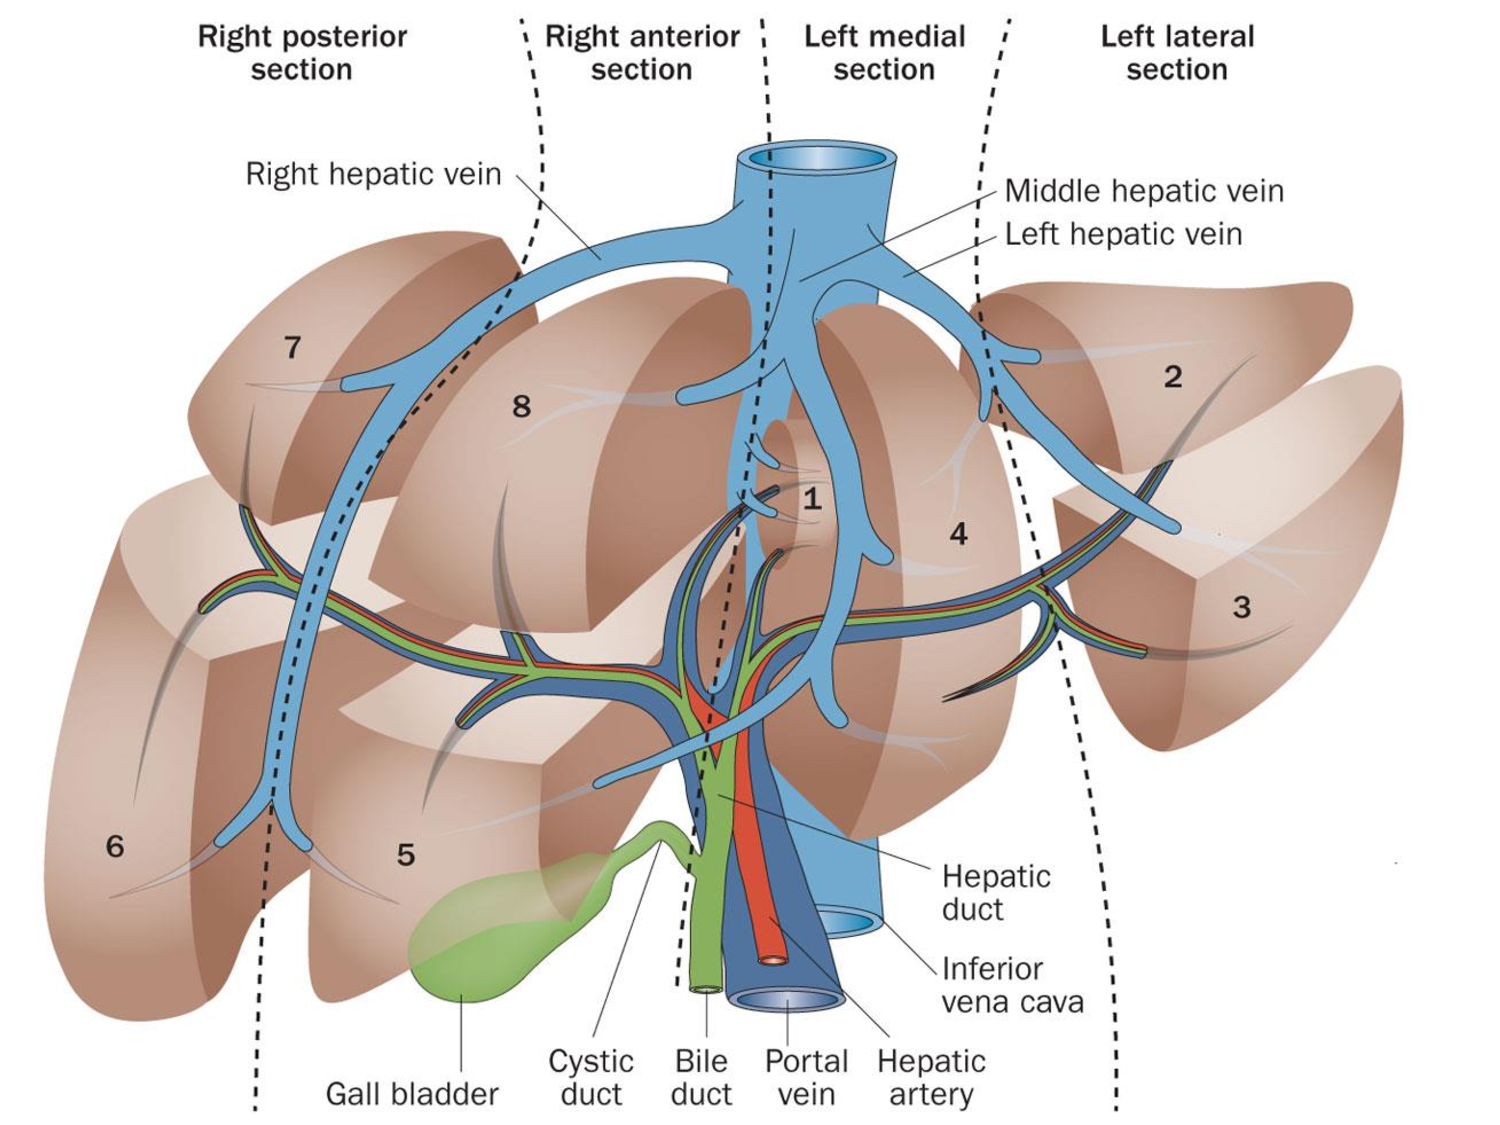
\includegraphics[width=\textwidth]{liverSegments}
  \caption{The liver and its eight Chouinaud segments. In red is the hepatic
    artery which transports blood from the heart a into the liver. In dark blue
    the portal vein, it transports blood from the gut into the liver. All the
    blood leavs the liver through the hepatic veins to the vena cava \cite{siriwardena2014management}.}
  \label{fig:liverSegments}
\end{figure}

\subsection{Liver Cancer}
\textcolor{green}{Liver metastatis are more common in US/Europe, in asia it's the other way around for example}

Liver cancer is cancer that starts in the liver. If the cancer has spread from
elsewhere to the liver, then it is known as liver metastasis. Liver metastasis
are about 20 times more common in the United States and in Europe than primary tumors. One of the reasons for that
is the rich blood supply of the liver which helps the tumors to grow
\cite{mcguire2016world}. In asia it's the other way round, more people suffer
from liver cancer than from liver metastases. Liver cancer patients often have chronic liver diseases
such as cirrhosis, problems of alcohol abuse, and viral hepatitis (B or C)
\cite{galun2015hepatocellular}. The gold standard to treat liver cancer are
surgical resections \cite{lencioni2012local}. The liver tissue can easily regrow, given that after resection there is
enough healthy tissue and blood supply preserved. Alternatively to resections
one can treat liver tumors by local ablation. Both variants treat the tumors
with a safety margin of 10 mm. This safety margin ensures that all tumor cells
are destroyed and to prevent further spread of cancer cells \cite{mahnken2009ct}.
\section{Liver Resections} 
\textcolor{green}{explain liver resections a bit more in detail, also what instruments are used and what to do with a blood vessel}
Hepatectomy is the surgical resection (removal of all or part) of the liver.
Liver resections are considered major surgeries and are done under general
anesthesia. If no other internal organs of the body are affected and the liver
is not cirrhotic, then 70\% to 80\% of the total liver volume can be removed in a
surgical resection. For patients with cirrhotic livers, not more than 50\% of
the total liver volume should be removed \cite{pianka2011liver}. Liver tissue is
cut using instruments like the BiClamp® vessel-sealing device (Figure \ref{fig:BiClampExplained}). Such devices can
simultaneously transect liver parenchyma and seal vessels with diameters smaller
than 7 mm \cite{zhao2017biclamp}. For larger vessels, resorbable clamps are used
to prevent undesired bloodflow out of the liver.
\begin{figure}[H]
  \centering
  \minipage{0.32\linewidth}
  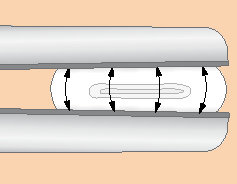
\includegraphics[width=\linewidth]{BiClamp1}
  \endminipage
  \hfill
  \minipage{0.32\linewidth}
  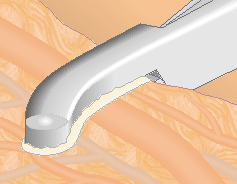
\includegraphics[width=\linewidth]{BiClamp2}
  \endminipage
  \hfill
  \minipage{0.32\linewidth}
  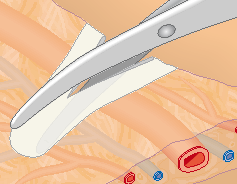
\includegraphics[width=\linewidth]{BiClamp3}
  \endminipage
  \hfill 
 \caption{A vessel sealing device is used to transect liver parenchyma and split
   blood vessels then seal them so that no blood is lost. From left to right:
   First, the vessel is pressed together and then the tissue coagulated using a bipolar
   electrosurgical current. In some cases this is done twice. Finally the tissue
   is separated mechanically at the center of the visible coagulation area \cite{biClampPdfWithImages}. }
  \label{fig:BiClampExplained}
\end{figure}

Most hepatectomies are done laparoscopicly. However for complicated
cases also open surgeries are done \cite{cherqui2000laparoscopic}. Two
resection techniques can be separated. Anatomical or parenchymal-sparing
resections (Figure \ref{fig:resectionsPlanning}). This work will concentrate on the latter technique. 
\begin{figure}[H]
  \centering
 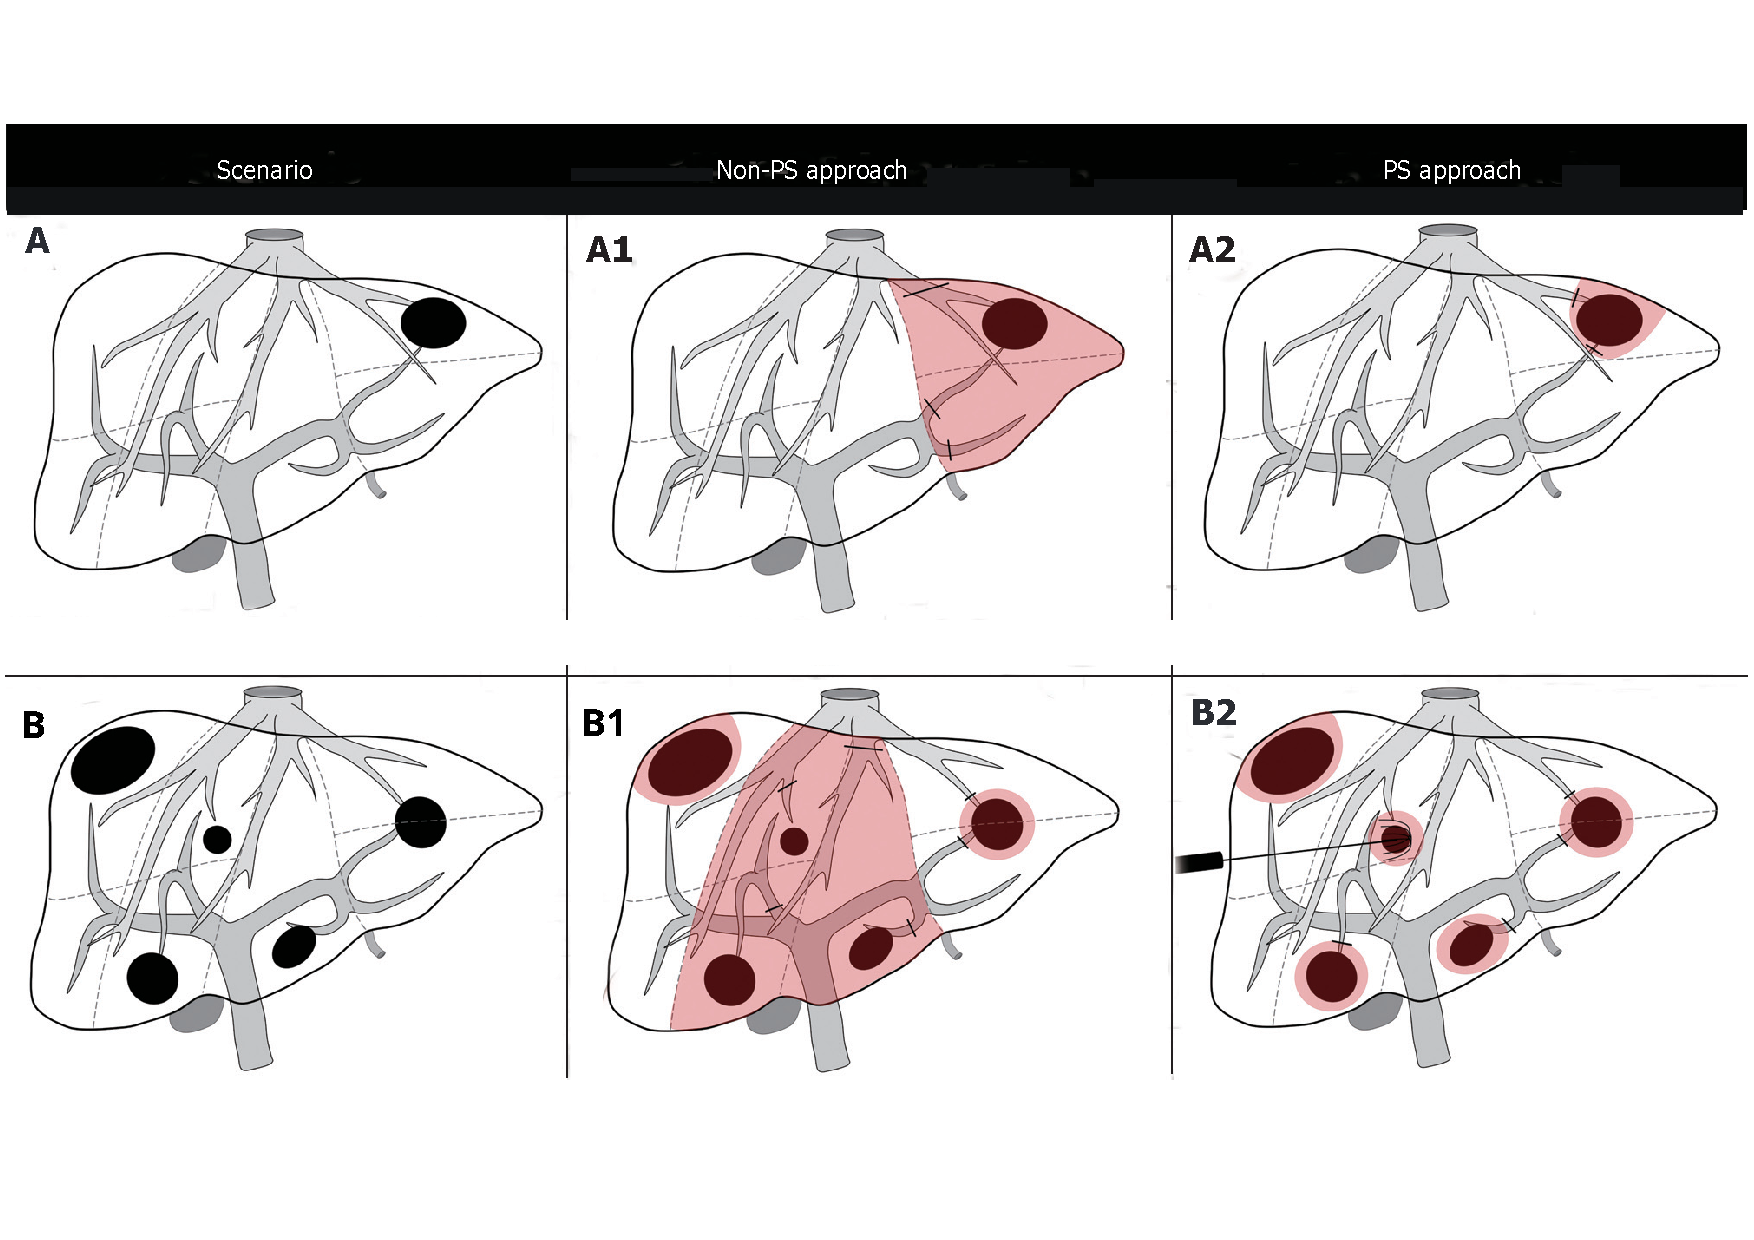
\includegraphics[width=\textwidth]{resectionsPlanning}
  \caption{Two different approaches to resect liver tumors in two different
    situations. The \textit{Scenario} column shows the situation of the
    patient's liver, the \textit{Non-PS approach} column shows how an anatomical
  resection plan would look like and the \textit{PS approach} column shows how a
parenchymal-sparing resection plan would look like \cite{alvarez2016parenchymal}.}
  \label{fig:resectionsPlanning}
\end{figure}


\subsection{Parenchymal-sparing liver surgeries}
Resection is the established gold-standard treatment of colorectal liver
metastases. The surgical treatment of colorectal liver metastases has changed with the expansion of the
parenchymal-sparing liver resection technique. This technique involves preserving healthy
functional liver parenchyma by performing a wide range of liver resections. In
order to perform the appropriate type of resection, the site and
relationships of the tumor with glissonian pedicles or hepatic veins have to be
known.
For that reason, it is obvious that only the heavy use of intraoperative liver
ultrasound makes it possible to perform parenchymal-sparing liver resections.
This can be also used with the laparoscopic approach. The method is backed by technical, oncological,
and pathological arguments.
This approach has multiple benefits: decreases postoperative mortality and
morbidity rates, while preserving the function of the liver. In turn, the risk
of liver dysfunction is reduced and the possibility of re-resection in case of
reccurence increases. Overall, parenchymal-sparing liver surgeries offer
similar survival results \cite{Ferrero2017}.
%\cite{alvarez2016parenchymal}
% \section{Objectives} 
% The objectives of this Master's thesis are:
% \begin{itemize}
%   \item Implementation of the concept for an intraoperative 3D reconstrction
%   technique of the liver from intraoperative ultrasound. 
%   \item Implementation of the intraoperative resection planning.
% \end{itemize}
% This work focuses on open surgical procedures of liver hepatectomies and
% especially parenchymal-sparing methods.


%Laparoscopic anatomical hepatectomy (LAH)

\section{Intraoperative ultrasound}
\textcolor{green}{Start with why US is used, then describe how it works and the limitations. from there you should have a nice transition to navigation}
In
liver surgeries an intraoperative ultrasound device is used for intraoperative planning and
navigation inside the liver. It is used to locate tumors that are not
visible on the liver surface and to estimate their sizes from the ultrasound image. Figure \ref{fig:liverUS} shows an example of an
ultrasound image of the liver and its corresponding position in the 3D liver
model.

\begin{figure}[H]
  \centering
 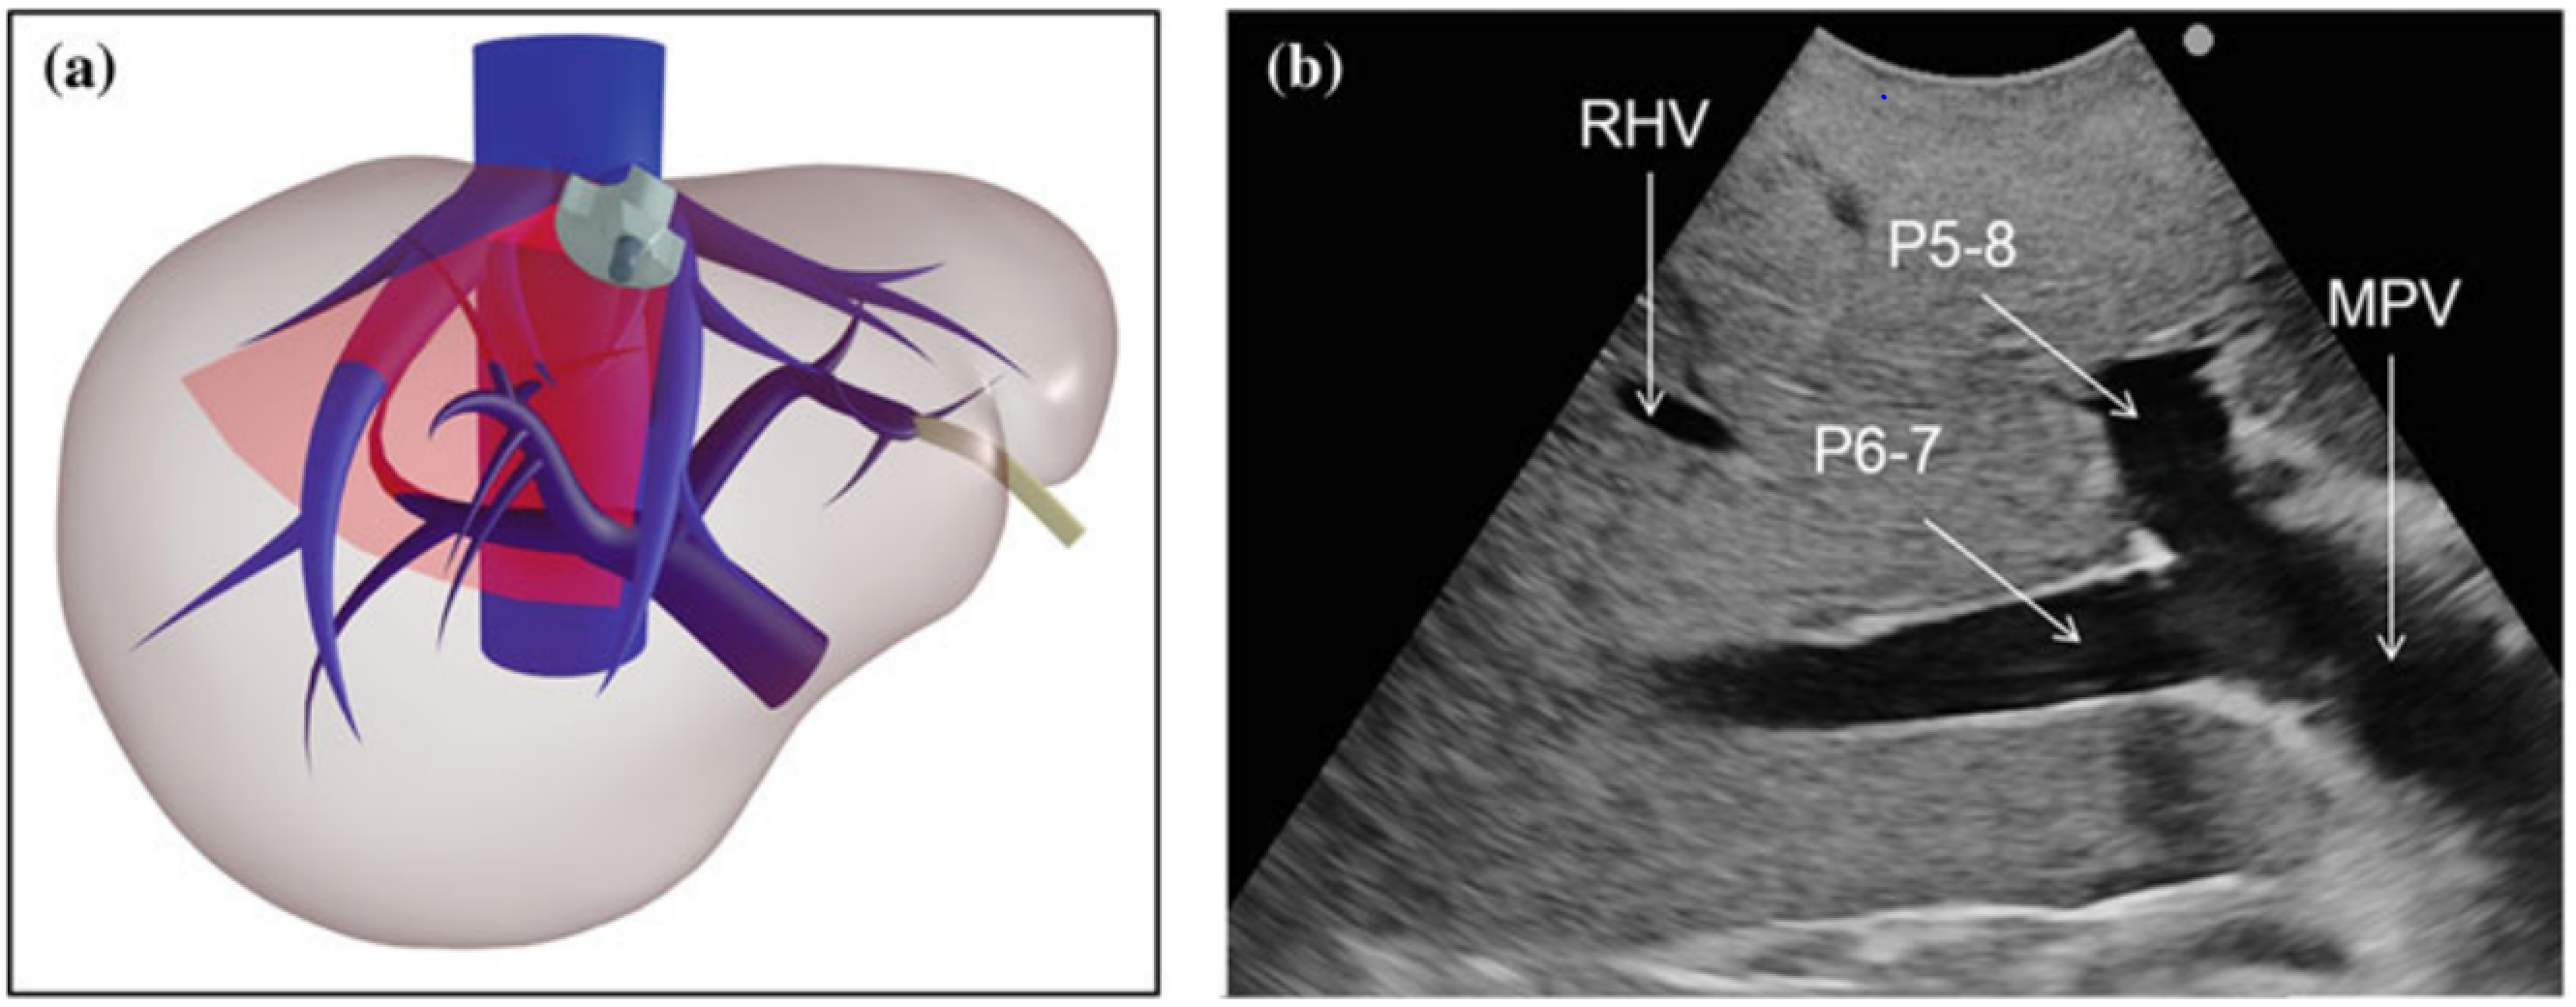
\includegraphics[width=\textwidth]{liverUS}
 \caption{ Left (a) ultrasound image plane in the liver. Right (b) intraoperative
   ultrasound image. One can see the right hepatic vein (RHV), the portal branch
   to segments 5 and 8 (P5-8) and the portal branch to segments 6 and 7 (P6-7) \cite{torzilli2014ultrasound}}
  \label{fig:liverUS}
\end{figure}

Ultrasound imaging works by the \textit{pulse-echo} principle. A short
ultrasound pulse is emitted from a transducer. The sound waves get
transmitted and reflected differently by different tissues. The reflected
 waves travel back into the transducer and are converted into an electrical
signal. After post-processing these signals become ultrasound images. 
The ultrasound measures the mechanical properties of the tissue. The tissues
have different acoustic impedance, which is the product of tissue density and
ultrasound speed in travelling through the tissue. The resolution of the
ultrasound images depends on the frequency of the ultrasonic waves. High
frequencies lead to higher resolution but lower penetration depth into the tissue because the
absorption of the sound energy increases with frequency too. Therefore the
useability to see deep structures is limited \cite{torzilli2014ultrasound}. 

In liver surgeries ultrasound is an important and established instrument.
Intraoperatively, the ultrasound is used on the liver surface directly,
therefore the penetration depth of the
ultrasound is optimal to represent the inner structures of the liver.
Registration methods based on 3D ultrasound reconstructed liver vessels 
exist but are not used in practice frequently \cite{lange2003vessel}. Ultrasound
is not harmful to health and therefore, can
be used as often as desired to navigate during a surgery.
% it is  
% Intraoperatively surgeons use ultrasound to localize the tumor as it gives
% advantages of reduced surgical time, complexity and radiation dosage.

\section{Navigation for liver resection surgeries}
\label{sec:navigationForLiverResections}
\textcolor{green}{first, why is navigation needed, then how does it generally work
  1) preoperative model or surgical plan 2) tracking 3) registration 4)
  navigation visualization etc. then challenges especially in liver surgery and limitations}
It is a difficult task for inexperienced surgeons to orientate themselves within the liver during an operation.
From the outside of the liver it is not visible where the blood vessels are which they do not want to hurt.
Navigation can help surgeons to orient themselves precisely in organs during
operations.

% The actual intervention in computer assisted surgeries (CAS) is defined as
% surgical navigation.
A navigated operation differs in a few points from a non-navigated operation.
Because every patient's liver is different, a new 3D model of the liver has to
be created before surgery. This models are created from pre-operative 3D
computer tomography (CT) scan of the liver. Then, using this model, a surgical plan is made.
In contrast to a regular operation, a navigation system is located in the
operating theatre and the surgical instruments can be tracked by it. Therefore special instruments are used. These
instruments have the ability to be tracked by the naviagation system. Depending
on the tracking technology used by the navigation system, the tools are different.
In order to also track the liver, the created model is registered to the anatomy
of the patient. Finally the orientation and position
of the instruments in relation to the patient's anatomy is visualized on a
monitor in the operating room. The surgeon can see what he does on the
monitor and uses the system to navigate the location and position of its
instruments. This is specialy then useful when the tip of the instrument is not
actually visible for the suergeon.

The achieved
navigation accuracy with such a system was 4.5 mm $\pm$3.6 mm averaged over nine surgeries \cite{peterhans2011navigation}.
Current research tries to compensate for deformations of the liver after the CT
scan to the actual shape of the liver \cite{clements2017deformation}
\cite{clements2015validation}. 
\subsection{Creation of preoperative 3D-models}
Several steps are necessary to create a preoperative model. First the 
CT scan is done. This leads to representations of the liver on several 2D images parallel
to each other, filling a square volume with voxels. From this data the liver and
its inner structures are manually segmented and merged to a 3D model (Figure \ref{fig:MeVisExample}). This is very
time consuming and therefore expensive \cite{numminen2005preoperative}.
Nevertheless the resulting models are very detailed and accurate.
\begin{figure}[H]
  \centering
 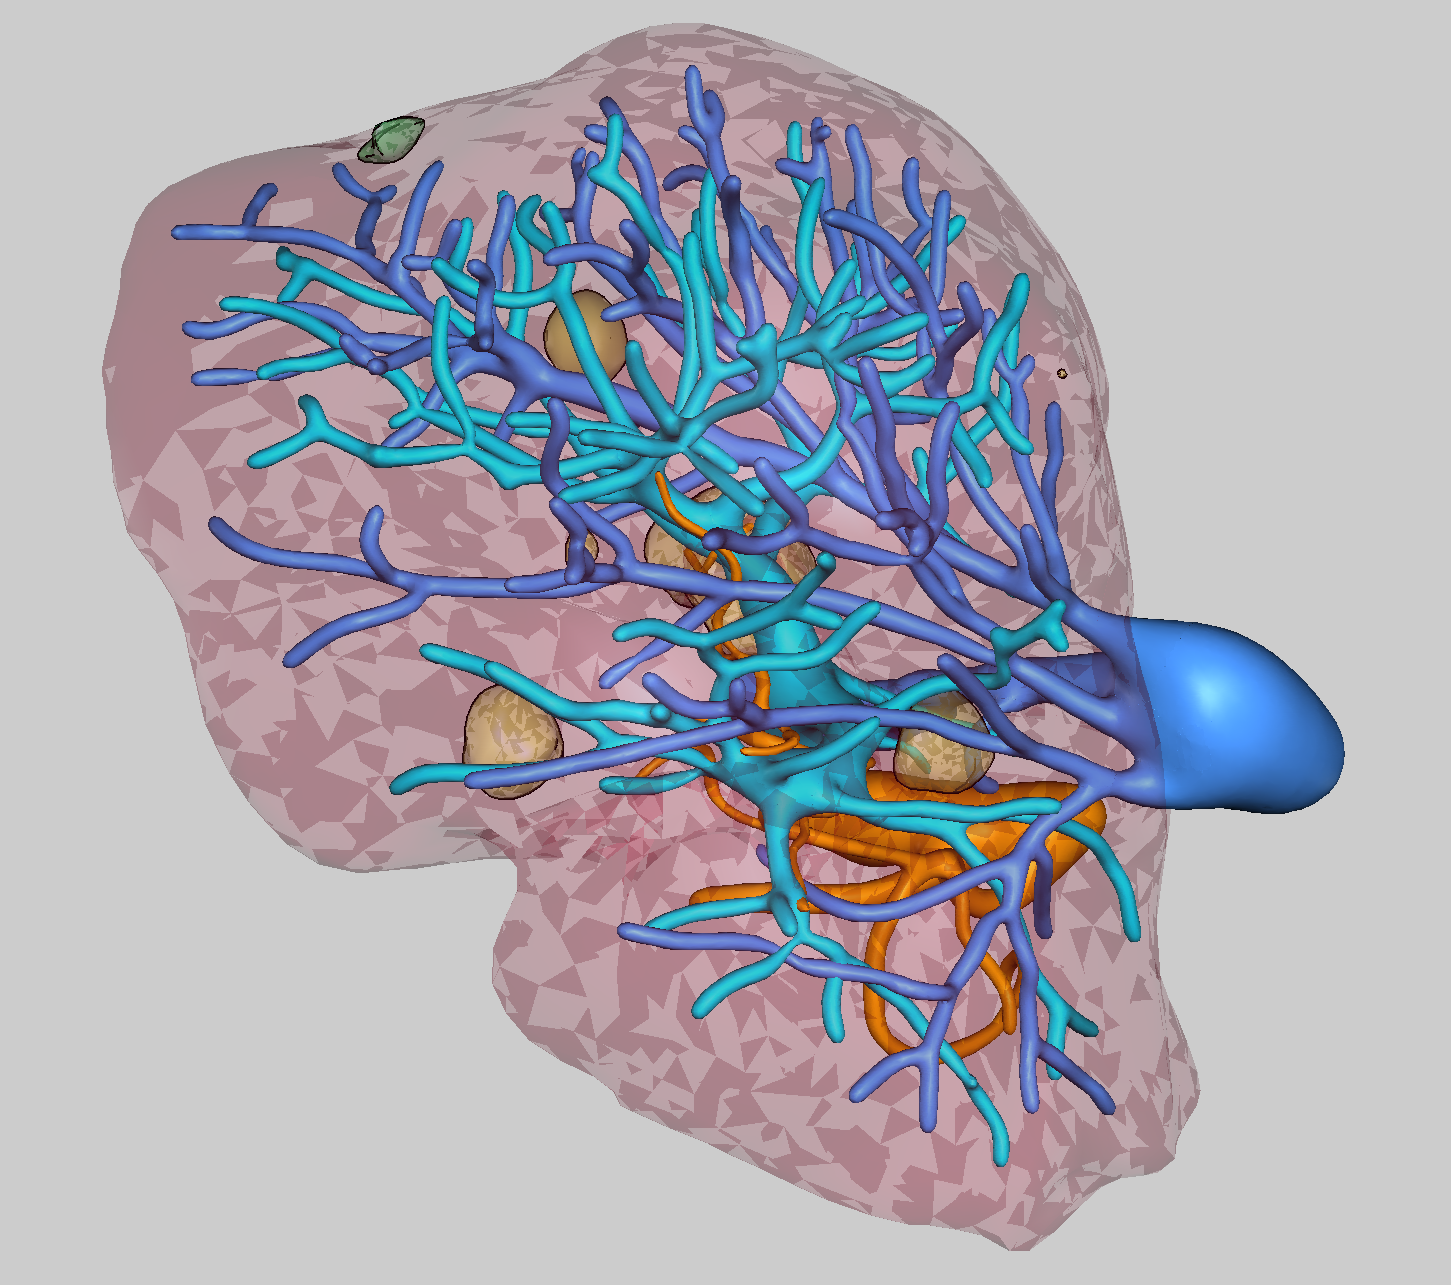
\includegraphics[width=0.6\textwidth]{MeVisExample}
 \caption{Example of a preoperative 3D model created by MeVis}%DK patient
  \label{fig:MeVisExample}
\end{figure}

\subsection{Registration methods}
Patient registration is a concept to correlate the reference coordinate system
of a virtual 3D data set with that of a patient. First, the 3D data set has to
be gathered. This is often done by CT or MRI scan of the patients anatomy to be
operated on. Secondly, finding of the transformation between the patient's
reference coordinate system and the virtual data set. During the surgery the patient is similarly
tracked as the instruments (see section \ref{sec:navigationForLiverResections}).
In this way, the patient has his own coordinate system. From here many different
methods exist to align the virtal data to the real anatomy.
Discrete landmarks, surface scans and
volumetric sonography scans are just a few of the approaches that can be
used to achieve precise alignment of the data with the
surgical site \cite{banz2016intraoperative}. 

\subsubsection{Surface registration}
Surface registration is registration based on surfaces. It is used and studied
for several years in all kinds of fields \cite{ramos2015review}. Especially in
the field of medical technology, a lot of research is being done in the
direction of contactless registration. Intraoperatively, different camera technologies which lead
to depth images are used to sample the surface of an organ. Often used imaging systems are stereo cameras
\cite{furukawa2010accurate}, structured light \cite{salvi2004pattern} and
laser range scanners \cite{cash2003incorporation}. From these intraoperatively
created data sets, surfaces are reconstructed and then used for registration. To
find the mapping between the surfaces, mostly different variants of the iterative
closest point (ICP) \cite{besl1992method} algorithm are used. 

These surface based methods are limited for different reasons. In most cases
only part of the whole organ can be seen (scanned). The scanned surface may lack
of unique structures on the surface. The scanning process can 
lead to noisy data. The organ of interest may be deformed between the
acquisitions of the surface samples. Therefore researchers try to compensate for
intraoperative soft-tissue deformations \cite{cash2005compensating}\cite{dagon2008real}.
\subsection{Tracking modalities}
To track surgical instruments and patient's anatomy (define the position and
orientation in real time) during naviagated surgery a tracking system is needed.
Tracking can be done by different technologies. The most used tracking
modality is optical tracking. 

\subsubsection{Optical tracking}
Optical tracking is the most used tracking modality in naviagated liver
surgeries. Passive markers (spherical, retro-reflective that reflect infrared
light) or active markers (infrared-emitting markers that are activated by an
electrical signal) \cite{wiles2004accuracy} are attached to the objects that
need to be tracked. A tracking camera is then emitting infrared light by illuminators
on the position sensor (only for passive markers). The position sensor
determines the position and orientation of the tracked instruments based on the
information it receives from those markers \cite{noauthor_polaris_nodate}.  
\endinput
%%% Local Variables:
%%% TeX-master: "MscThesis"
%%% End:
\chapter{State of the art}

\section{Intraoperative ultrasound}
Ultrasound imaging works by the \textit{pulse-echo} principle. A short
ultrasound-pulse is emitted from a transducer. Then the soundwaves get
transmitted and reflected differently by different tissues. The reflected
soundwaves travel back into the transducer and get converted into an electrical
signal. After post-processing these signals become ultrasound images. Basically
the ultrasound measures the mechanical properties of the tissue. The tissues
have different acoustic impedance, which is the product of tissue density and
ultrasound speed in travelling through the tissue. The resolution of the
ultrasound images depends on the frequency of the ultrasound waves. High
frequencies lead to high resolutions but low depth into the tissue because the
absorption of the sound energy increases with frequency too. Therefore the
useability to see deep structures is limited \cite{torzilli2014ultrasound}.

\section{Navigation for liver resections}
Navigation in liver surgeries is mostly done by registering the patient to a pre-operative 3D
computer tomography (CT) scan of the liver during the surgery. All surgical
instruments have trackable markers attached to them. A tracking camera sees
these markers and can differentiate the different instruments from their attached
markers. The achieved
navigation accuracy was 4.5 mm $\pm$3.6 mm averaged over nine surgeries \cite{peterhans2011navigation}.
Current research tries to compensate for deformations of the liver after the CT
scan to the actual shape \cite{clements2017deformation}
\cite{clements2015validation}. 

\subsection{Registration methods}
Different registration methods exist. Discrete landmarks, surface scans and
volumetric sonography scans are just a few of the approaches that can be
used to achieve precise alignment of the preoperative image data with the
surgical site \cite{banz2016intraoperative}.

\subsection{Tracking modalities}
To track surgical instruments and patient's anatomy (define the position and
orientation in real time) during naviagated surgery a tracking system is needed.
Tracking can be done by different technologies. The most used tracking
modality is optical tracking. 

\subsubsection{Optical tracking}
Optical tracking is the most used tracking modality in naviagated liver
surgeries. Passive markers (spherical, retro-reflective that reflect infrared
light) or active markers (infrared-emitting markers that are activated by an
electrical signal) \cite{wiles2004accuracy} are attached to the objects that
need to be tracked. A tracking camera is then emitting infrared light by illuminators
on the position sensor (only for passive markers). The position sensor
determines the position and orientation of the tracked instruments based on the
information it receives from those markers \cite{noauthor_polaris_nodate}.  

\section{Surface reconstruction}
A surface reconstruction's goal is to create a surface from sampling points. Two
main steps need to be processed. First, collecting the sample points. Second,
apply a reconstruction algorithm to the sampled points. There exist different
methods of collecting surface points
\cite{franca20053d}\cite{levoy2000digital}\cite{cui20113d}\cite{chu2002infrared}\cite{dou20153d}.
Optical (non-contact scan) scans are the most popular ones. Specialy laser based
scanners can scan very fast and with a precision in the order of micrometers. Also contact scans exist
\cite{pai2001scanning}. Contact scans can also be very precise (in the order of
micrometers).
The resulting sampling points lie on or near an unknown surface. A
reconstruction algorithm has now to reconstruct the surface from these points.
Again, a lot of reconstruction algorithms exist \cite{lim2014surface}. Only a
few articles were published in the
field of liver surface scanning \cite{maier2014comparative} \cite{thompson2015accuracy}. 



% \begin{itemize}
%   \item not tracked laproscopic one shot images stereo with registration
%   \item moved laproscopic tracked endoscope stereo with registration 
% \end{list}

% \cite{hoppe1992surface}

\endinput
%%% Local Variables:
%%% TeX-master: "MscThesis"
%%% End:
\chapter{Problem Statement}

\endinput
\chapter{Concept}
In this chapter the desired concept will be presented. 
\section{System}
The hardware used with this system consists of:
\begin{itemize}
  \item a tracked ultrasound device
  \item a tracked pointer tool
  \item an optical tracking camera to track the instruments
  \item a computer to run the software
  \item a 3D-monitor which displays the 3D contents of the software 
  \item a touch-screen on a 2D-monitor to operate the software and show the
    ultrasound images
\end{itemize}
The software in this system consists of:
\begin{itemize}
  \item a sampling method to collect points on the liver-surface
  \item a reconstruction method to reconstruct the surface from the sampled points
  \item a segmentation method to segment the tumors on the ultrasound images
  \item a planning method to plan the resection of the liver
  \item a navigation mode used to navigate during the removal of the tumor
\end{itemize}
\section{Functionalities}
The three main functionalities of the developed concept will be presented in
this chapter. These functionalities were specifically developed for this project.
\subsection{Surface Reconstruction}
During surgery ultrasound images and their corresponding 6D poses (positions and
orientations) are collected and analyzed. First each ultrasound image has to be
checked for contact with the liver. If the ultrasound passes the check, that
means the ultrasound image looks like an ultrasound image that can only arise
when the ultrasound probe lies on the liver surface, then the position of this
image can be used.

In order to use the sampled position corresponding to an image, this
position has to be transformed into the correct coordinate system first. There
are four different coordinate systems. The first coordinate system is the image
coordinate system. The units in the image coordinate system are pixels and the
origin is in the top left corner of the image. The
second coordinate system is the ultrasound coordinate system. The origin of this
coordinate system is at the probe tip in the middle and the units in this and
the following coordinate systems are millimeters. The third coordinate system is the
ultrasound-tool-marker coordinate system. The origin is ... . The final
coordinate system is the tracking camera coordinate system. The origin of this
coordinate system is at the position sensor in the tracking camera and can not
be changed.

At the end of this transformation chain, a image pixel 2D position was
transformed into a tracking camera 3D positon and the units changed
from pixel to millimeter. This 3D location in the tracking camera coordinate system
will be added to the collection of points to later reconstruct the surface from.

After collecting the surface points, the reconstruction algorithm from Hoppe
\cite{hoppe1992surface} reconstructs the surface from these points.
\subsection{Tumor Segmentation}
To reconstruct and later plan the resection of a tumor, the shape
of the tumor has to be made visible first. Because most liver tumors are not visible from the outside of the liver, an
ultrasound device is mostly used during liver resections to look behind the
liver surface.
Most tumors have roundish shapes and a sphere is the easiest
geometrical shape that can be used to approximate a tumor's real shape. To
define a sphere two components are needed: the location and the radius of the
spere.
To find the location of the tumor, the surgeon locates the tumor with the
ultrasound. Then he freezes the ultrasound image that cuts through the middle of
the tumor. The 6D pose of that ultrasound image is stored and the image is
passed to the next step. The tumor on the image has to be segmented. This
segmentation is done semi automatically. That means the surgeon has to
roughly initialize the segmentation manually and then the graph cut algorithm
implemented by openCV will segment the the tumor. From the resulting
segmentation shape, the tumor center and radius are estimated. The center
corresponds to the mean of the segmented boarder pixels and the radius is the
mean between the largest and the shortest distance from the boarder pixels to
the estimated center pixel. By using the 6D pose corresponding to the ultrasoud
image used for the segmentation, the center pixel gets transformed into the
tracking camera coordinate system. Finally the sphere that approximates the
tumor can be drawn into the same coordinate system as the liver surface.
\subsubsection{Automatic 3D}

\subsection{Resection Planning}
For parenchymal-sparing liver resections, the goal is to keep as much healthy tissue as
possible. When the location in the liver and the size of the tumor are known, one can plan a
precise resection from these informations.
% After collecting the needed
% information as described in the previous sections, the planning can 

\section{Workflow}
In this chapter the conceptual workfolw through a liver resection using the
desired system will be presented.
\subsection{Resection planning for non-anatomical ...}

%%% Local Variables:
%%% TeX-master: "MscThesis"
%%% End:
\chapter{Implementation}
This chapter will explain how the described concept has been implemented.
First an overview of the concept and then the main parts of the software in more
detail.
The trackable marker is attached to the ultrasound probe. The marker is
detectable by the tracking camera and enables the camera to determine the
position and orientation of the ultrasound probe. The probe on its own will
create an ultrasound image. Then the sampled ultrasound image and pose will be
post processed as a pair in the computer. In the software, depending on the
actual state of the surgery, the use of the two will be different.

\begin{figure}[H]
  \centering
 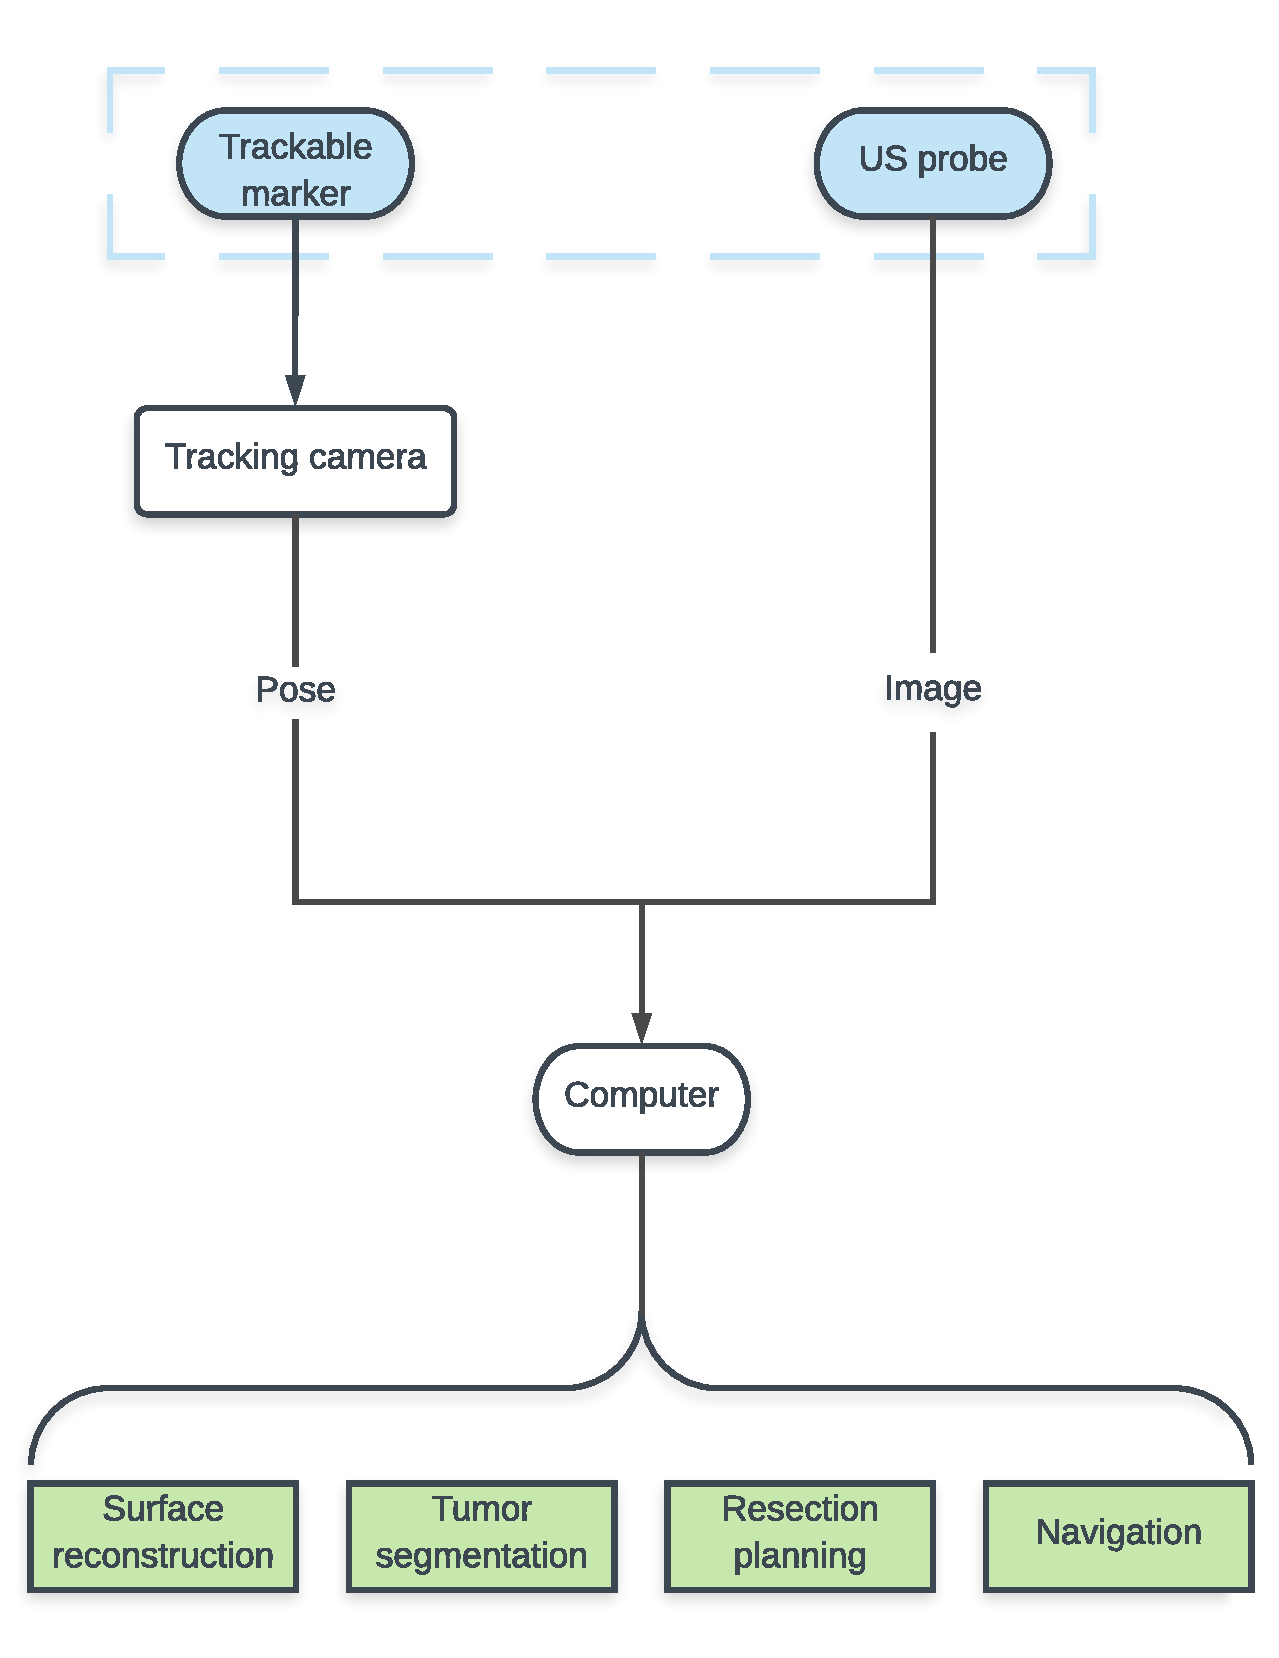
\includegraphics[width=0.65\textwidth]{FirstFlowChart}
  \caption{The way of the ultrasound image and the corresponding pose to the
    computer and later to the different parts in the software.}
  \label{fig:FirstFlowChart}
\end{figure}

\section{Surface Reconstruction}
While the surgeon is scanning the surface, the software in the background
filters out unusable positions. An image pose pair has to take two hurdles to
become accepted in the group of surface points. The image has to prove that it
arised from the liver surface and the position has to have a similar distance to
its neighbors as its neighbors to it. 
When enough points are sampled, the reconstruction of the surface will be
carried out.
\begin{figure}[H]
  \centering
 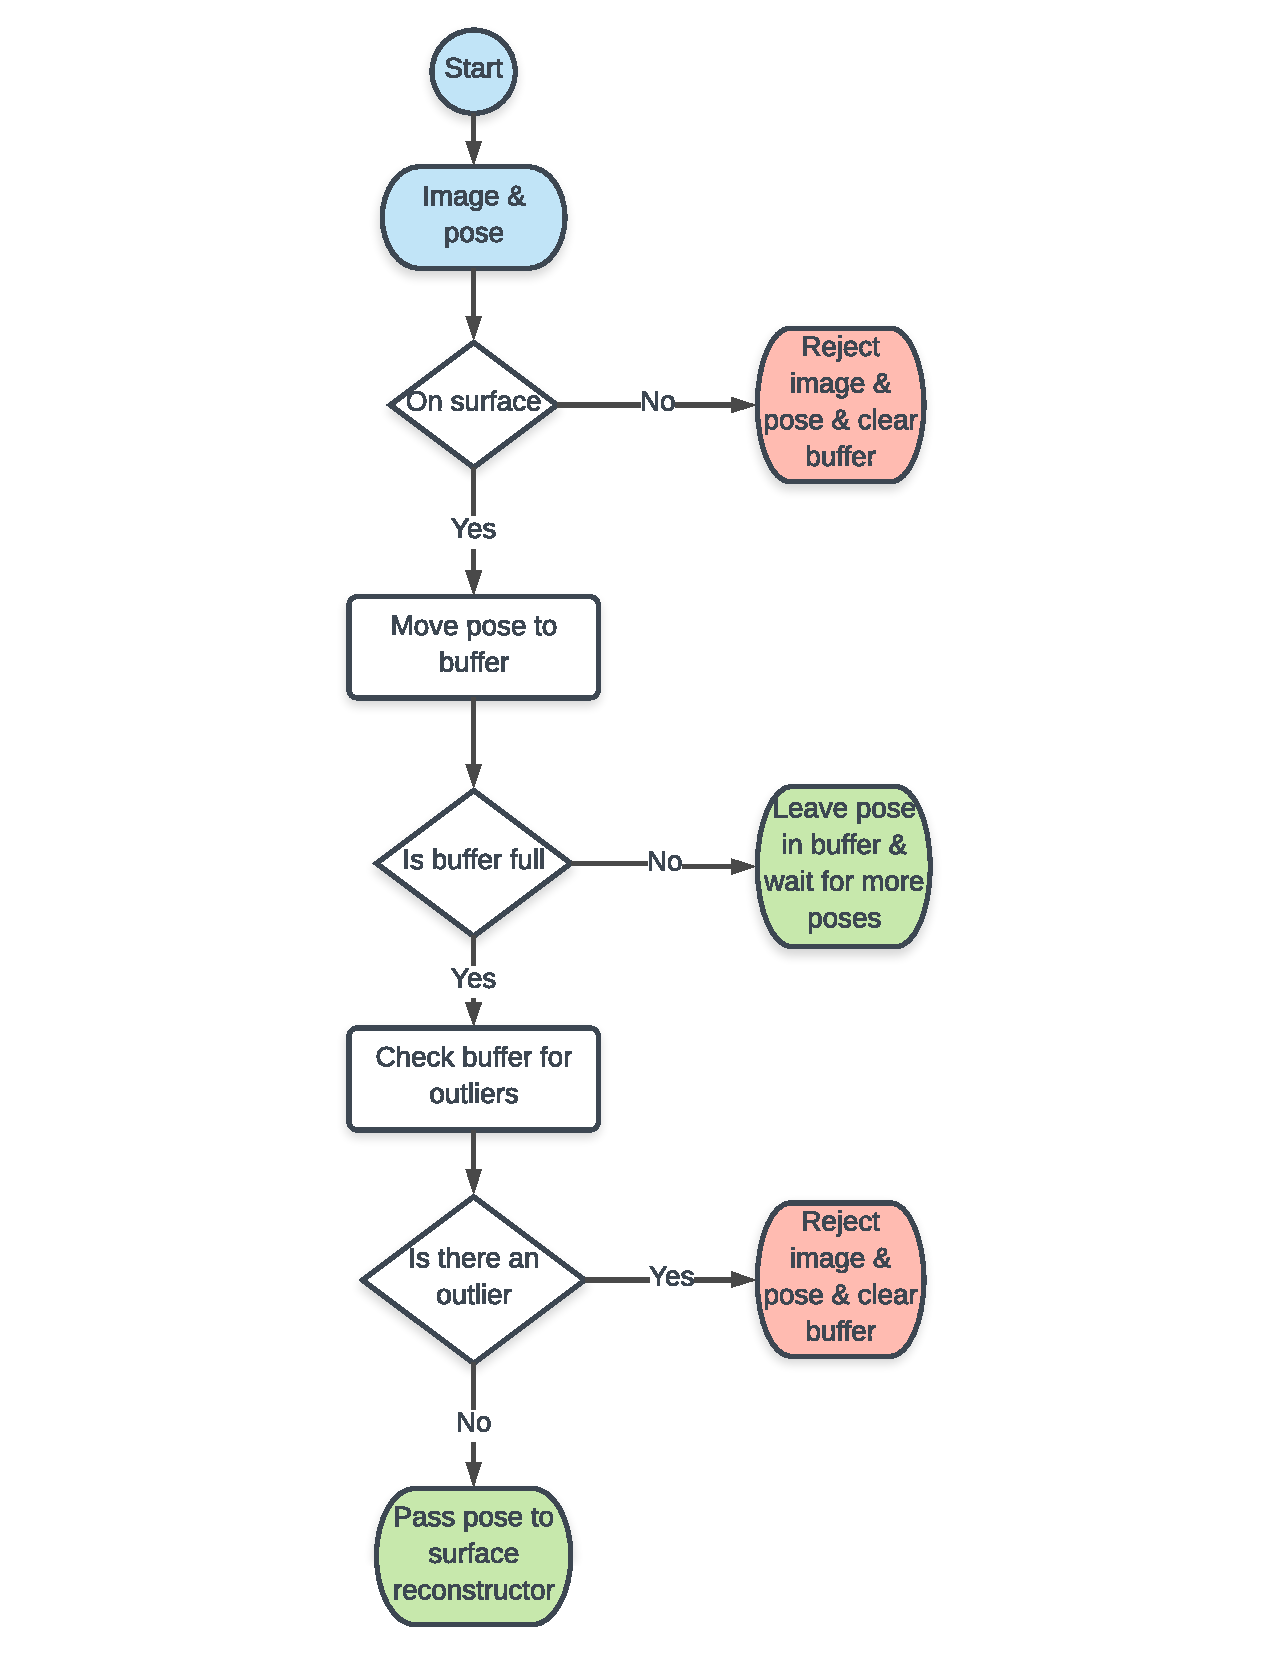
\includegraphics[width=0.65\textwidth]{SecondFlowChart}
  \caption{The way of the image and its pose if the surgeon is scanning the
    surface.}
  \label{fig:SecondFlowChart}
\end{figure}

\subsection{Surface contact detection}
For an image pose pair, the first step to pass is the contatct detection. Only
the ultrasound image is needed in this step. 

\begin{figure}[H]
  \centering
  \minipage{0.32\linewidth}
  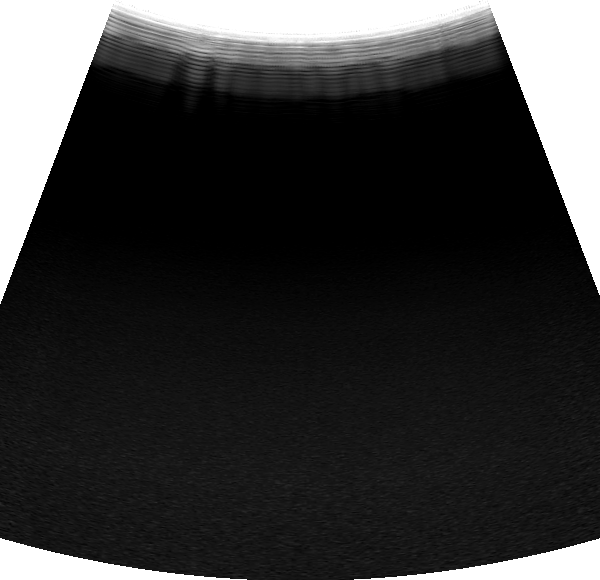
\includegraphics[width=\linewidth]{contact_no}
  \endminipage
  \hfill
  \minipage{0.32\linewidth}
  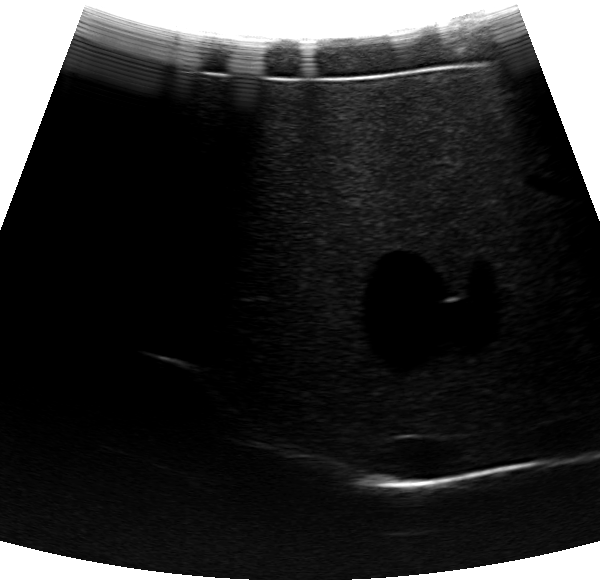
\includegraphics[width=\linewidth]{contact_difficult}
  \endminipage
  \hfill
  \minipage{0.32\linewidth}
  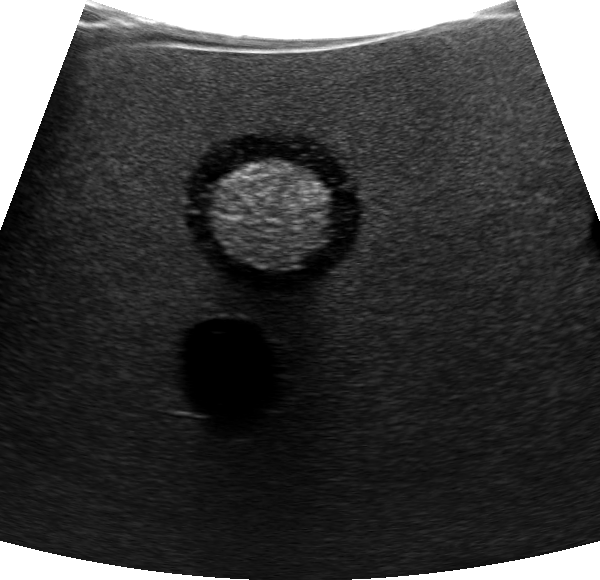
\includegraphics[width=\linewidth]{contact}
  \endminipage
  \hfill 
 \caption{Three ultrasound images from left to right: No contact with the liver,
   difficult to decide (In this case it would be contact because the middle part
   of the image shows contact), contact with the liver}
  \label{fig:contactVSnocontact}
\end{figure}

A classifier detects whether the US probe has contact to the liver or not. Therefore, a support vector machine (SVM) was trained with US images
from the phantom and from previous navigated liver surgeries. The SVM was trained to
classify the image into ``no surface contact'' (left) and ``surface contact'' (middle and right).
The images were labelled as "surface contact" if at least 50\% and the center had contact
to the surface (Figure 6.4 middle). The classifier takes into account that US waves are
reflected at the US probe-air interface when the US probe has no contact to the liver and
therefore no image is formed. The features for the classifier were: mean, median, minimum,
maximum, variance, skewness and kurtosis of the pixel values. All features are calculated
on the upper half of the image. For training, a set of 2'311 images (1'056 with contact, 1'255
without contact) were used. The training data was composed of images from a phantom
(88\%) and images from previous navigated liver surgeries (12\%). All computations were
performed using the SciPy software package. When the image is classified as ``surface contact'', then the position of the pose is stored
into the buffer. The buffer has a capacity of 10 positions. When
the addition of the actual pose leads to a full buffer, the buffer is
tested for outliers.
Each time a ``no surface contact'' image is classified and the positions buffer
is not empty it gets cleard.
\subsection{Outlier removal}
To find outliers in the current buffer the local
outlier factor is calculated for each position. 

\subsubsection{Local outlier factor}
The local outlier factor is a numerical value that describes the local density
of a position compared to its k-nearest neighbors (Figure
\ref{fig:lofExample}).

\begin{figure}[H]
  \centering
 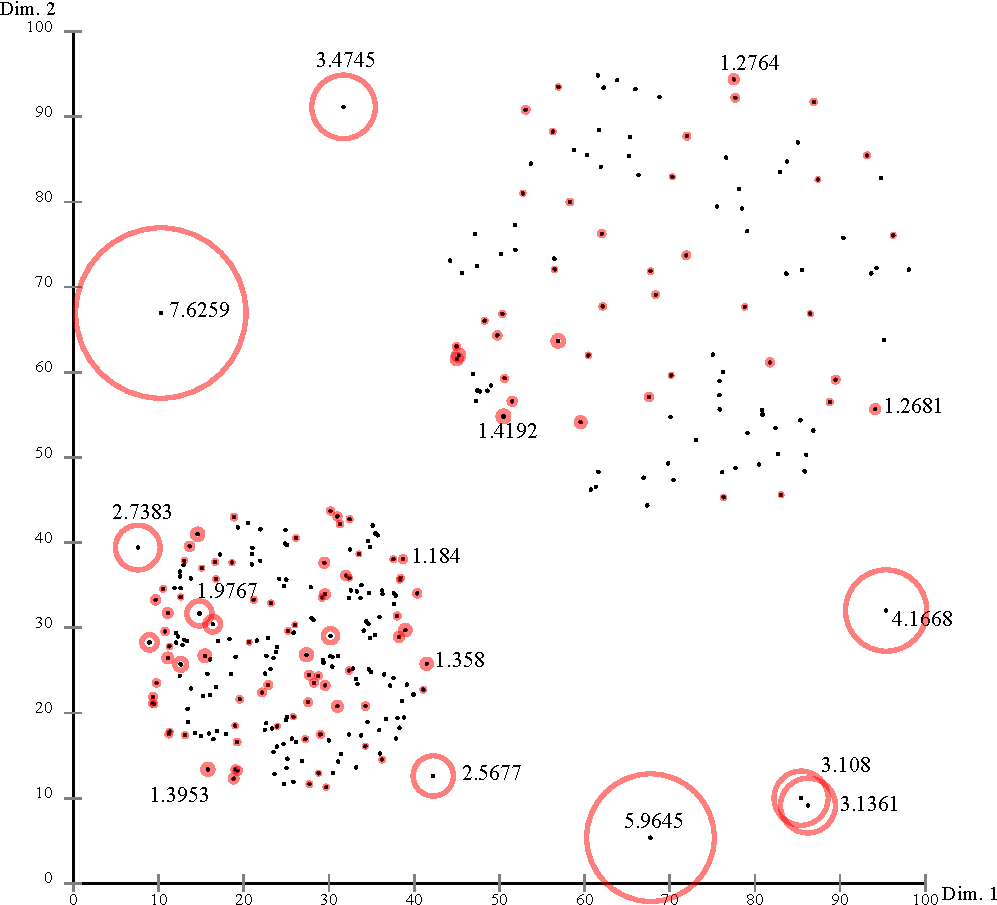
\includegraphics[width=0.6\textwidth]{lofExample}
  \caption{Example of the local outlier factors in a two dimensional pointcloud \cite{pictureLOF}.}
  \label{fig:lofExample}
\end{figure}

Five steps can be separeted to find the LOF of one position.
\begin{enumerate}
  \item{For each point calculate the distance to all the other points in the buffer}
  \item{For each point find the distance to his k-nearest neighbor $\rightarrow$
      \textit{k-distance}}
  \item{Find the \textit{reachability distance} from the k-nearest neighbors
      of each point to it self}
  \item{Calculate the \textit{local reachability density} for all points}
  \item{Calculate the \textit{local outlier factor}}
\end{enumerate}
The \textit{reachability distance} of point $A$ from another point $B$ is defined:
\begin{gather*}
  \mbox{reachability-d}_k(A,B)=\max\{\mbox{k\_d}(B), \mbox{d}(A,B)\}
\end{gather*}
The \textit{k-distance} of point $B$ depends on its k-nearest neighbors
and does not need to include point $A$.
But the actual distance between point $A$ and $B$ depends on only $A$
and $B$. The larger of the two will be the \textit{reachability distance} of
point $A$ from point $B$.

The \textit{local reachability density} of a point $A$ describes its neighborhood
and is defined by:
\begin{gather*}
  \mbox{LRD}(A):=1/\left(\frac{\sum_{B\in kNN(A)}\mbox{reachability-d}_k(A, B)}{|kNN(A)|}\right)
\end{gather*}
In words this is the inverse of the sum of the \textit{reachability distances} of point $A$
from its k-nearest neighbors devided by $k$.

Finally the \textit{local outlier factor} of a point $A$ indicates how his
neighborhood compares with the neighborhoods of his k-nearest neighbors. The LOF
of $A$ is defined by:
\begin{gather*}
  \mbox{LOF}(A):=\frac{\sum_{B\in kNN(A)}\frac{\mbox{LRD}(B)}{\mbox{LRD}(A)}}{|kNN(A)|}
\end{gather*}
If the neighborhood of $A$ is very similar to the neighborhoods of its k-nearest
neighbors, the LOF is close to 1. If its neighborhood is less dense than the
neighborhoods of his k-nearest neighbors, the LOF becomes larger than 1. If its
neighborhood is more dense than the neighborhoods of his k-nearest neighbors,
the LOF becomes lower than 1. \\
 \\
If an outlier is found in the buffer, the whole buffer is cleared. In the case
that no outlier is found, the oldest pose in the buffer gets moved into the
point collection to reconstruct the surface from.
\subsection{Reconstruction Parameters}
Finally there is a pointcloud with all the collected positions. This pointcloud
will be used as input for the surface reconstruction algorithm by Hoppe
\cite{hoppe1992surface}. The algorithm consists
of three phases. From an unorganized set of points, phase 1 constructs an
initial dense mesh. Starting with the dense mesh created in phase 1, phase 2
reduces the number of faces and improves the fit to the data points. In phase 3,
the surface representation is changed from a piecewise linear one (meshes) to a
piecewise smooth one. For the computations the implementation in VTK
(SurfaceReconstructionFilter) was used. The two main parameters of this
reconstruction algorithm have been optimized by applying the grid search method.
\subsubsection{Grid search for parameter optimization}
The \textit{neighborhood size} and the \textit{sample spacing} are the variable
parameters of the used surface reconstruction algorithm. The \textit{neighborhood size}
specifies the number of neighbors each point has. These neighbors are used to
estimate the local surface orientation. The \textit{sample spacing} sets the
spacing of a 3D sampling grid.
To find the optimal values to use in the algorithm with the point cloud data produced in the
experiment described in section \ref{sec:SurfaceReconstructionAccuracy}, a
first, rough grid search has been done to find the range of interest
of the two parameters. The same data was then used to do a second, more dense
grid search over the range of interest (Figure \ref{fig:gridSearchResultMean} and
\ref{fig:gridSearchResultSTD}). For each parameter setting, the average distance from the
reference points to the reconstructed surface was calculated.
\begin{figure}[h]
  \centering
 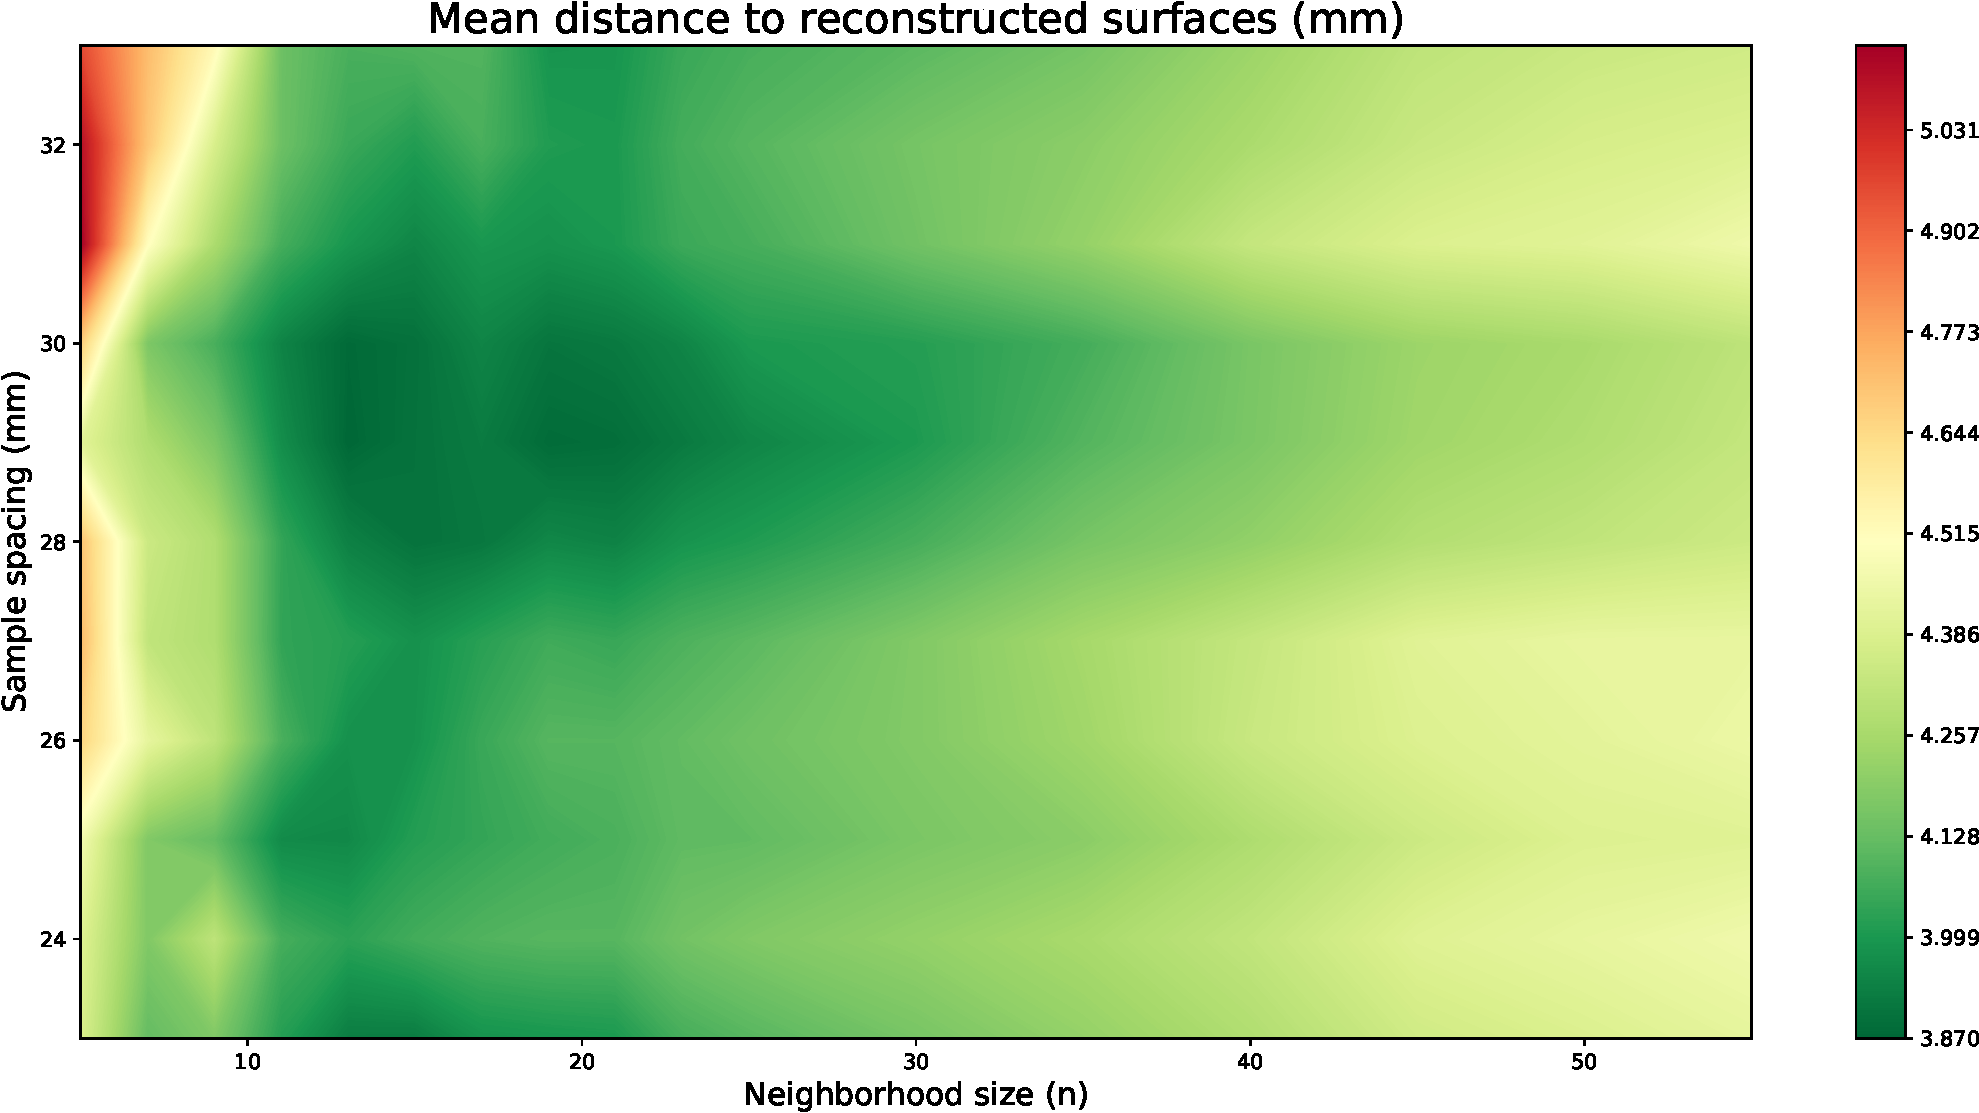
\includegraphics[width=0.9\textwidth]{gridSearchResultMeanCrop}
  \caption{This contour plot shows the mean distance calculated over 10
    differently sampled point collections. All point collections represent the
    surface of the same liver phantom.}
  \label{fig:gridSearchResultMean}
\end{figure}
The found mean distance varies from 5.1 mm to 3.9 mm. Neighborhood sizes smaller
than 8 show an increase of the mean distance for sample spacings larger than 25
mm. Neighborhood sizes over 30 seem to increase the mean distance also.
The standard deviation of the mean varies between 6.1 mm and 4.6 mm. These high
deviations result mostly from the boarder part of the reconstructions where the
reference points are more than 2 cm away from the surfaces (see section
\ref{sec:SurfaceReconstructionAccuracy}). One can say the standard deviation of
the mean decreases together with the neighborhood size used for the
reconstruction. But this is only true for neighborhood sizes larger than 13.
Because from neighborhood size 13 till 10 the standard deviation increases not
till then it decreases again. 
\begin{figure}[h]
  \centering
 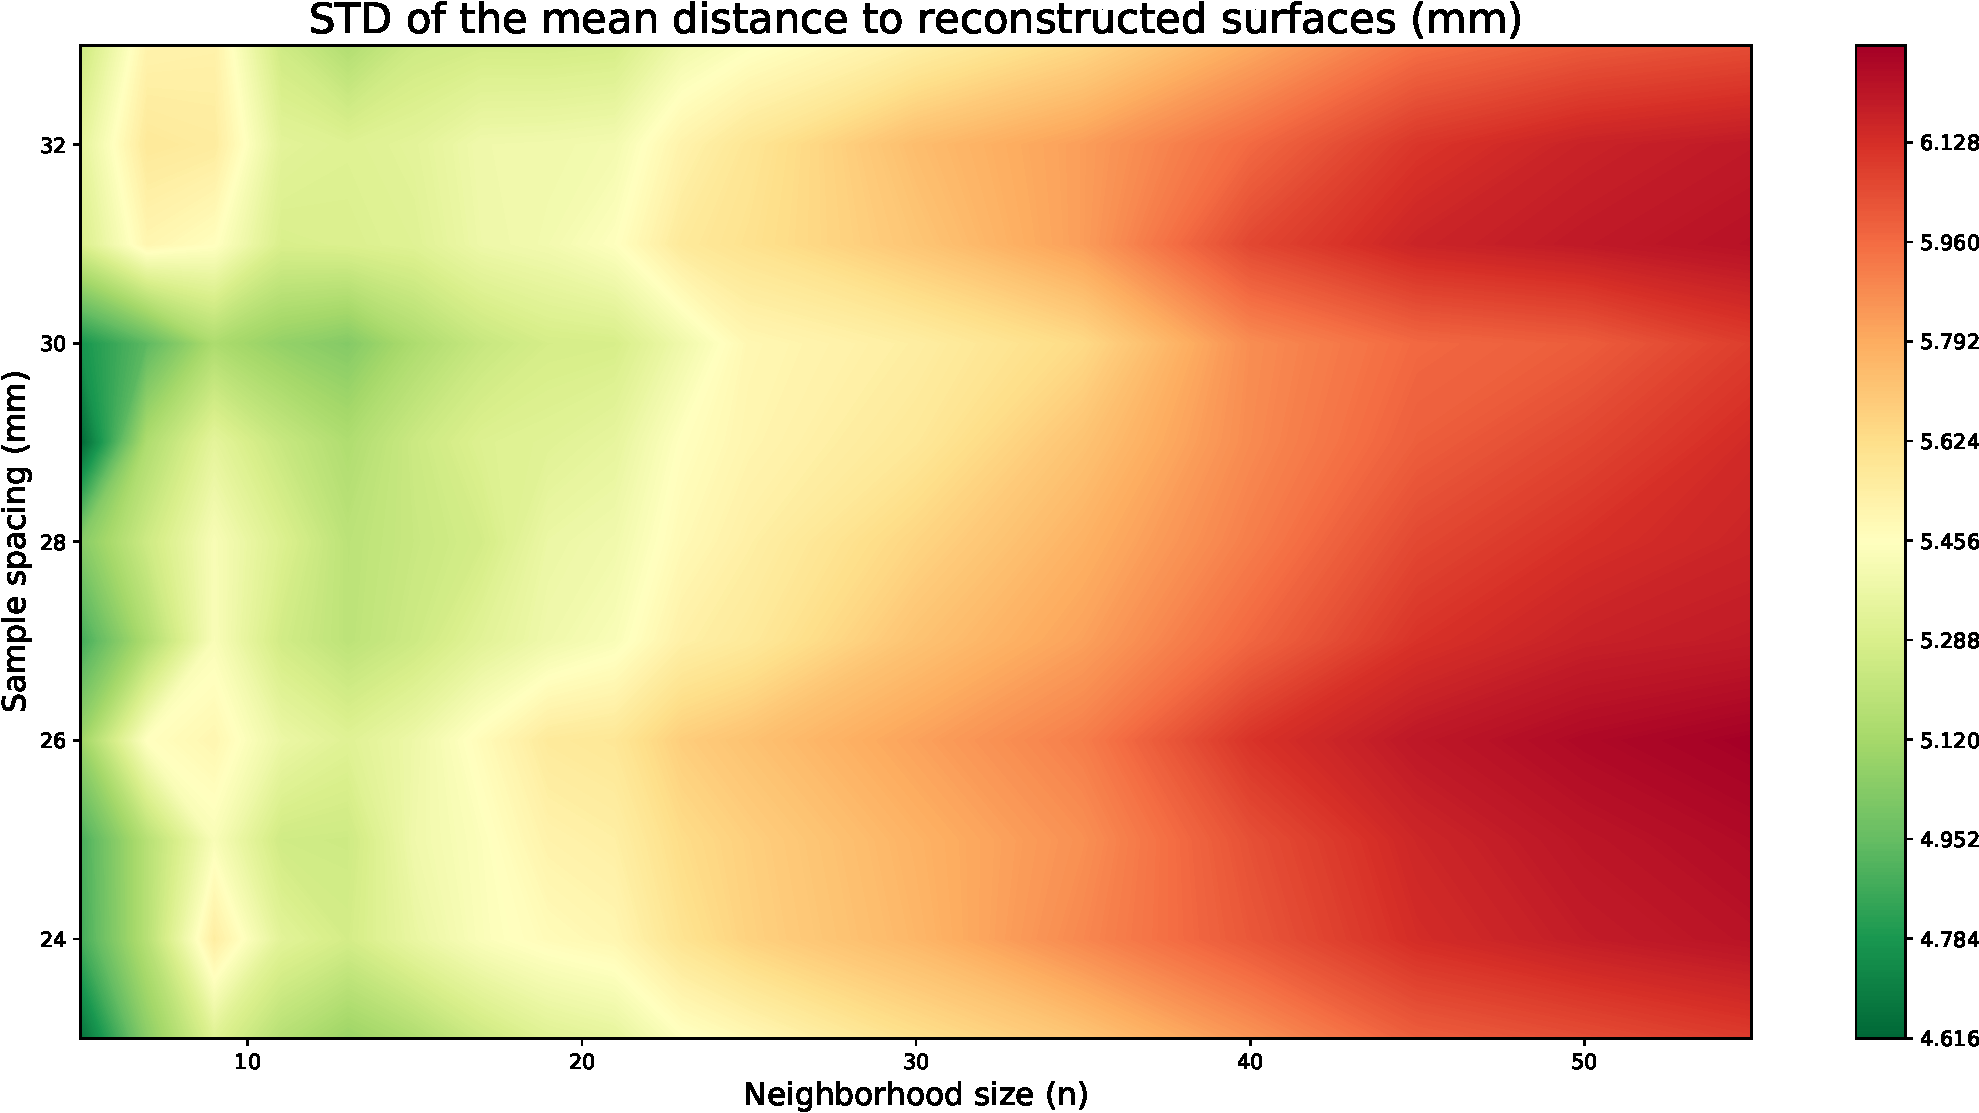
\includegraphics[width=0.9\textwidth]{gridSearchResultSTDCrop}
  \caption{This contour plot shows the STD of the mean distance calculated over 10
    differently sampled point collections. All point collections represent the
    surface of the same liver phantom.}
  \label{fig:gridSearchResultSTD}
\end{figure}
By simply summing up the mean and the standard deviation, one finds that the
optimal parameters for the tested surface samplings are 13 for the neighborhood
size and 30 mm for the sample spacing.
\section{Tumor Segmentation}
\label{sec:tumorSegmentation}
The flow diagram in figure \ref{fig:ThirdFlowChart} helps to understand the
following explanation of the creation of a tumor 3D model.
To create a 3D model of a tumor, the surgeon has to freeze an ultrasound image
such that the real tumor center is visible on this image. To find the location
of the tumor's center, the surgeon locates the tumor with the
ultrasound. Then he freezes the ultrasound image that cuts through the middle of
the tumor. The 6D pose of that ultrasound image is stored and the image is
passed to the next step.

Most tumors have roundish shapes. and a sphere is the easiest
geometrical shape that can be used to approximate a tumor's real shape. To
define a sphere two components are needed: the location and the radius of the
spere.

To get more information about the tumor, the tumor on the freezed image has to be segmented. This
segmentation is done semi automatically. That means the surgeon has to
roughly initialize the segmentation manually and then the graph cut algorithm
implemented by openCV will segment the the tumor. From the resulting
segmentation shape, the tumor center and radius are estimated. The center
corresponds to the mean of the segmented boarder pixels and the radius is the
mean between the largest and the shortest distance from the boarder pixels to
the estimated center pixel. By using the 6D pose corresponding to the ultrasoud
image used for the segmentation, the center pixel gets transformed into the
tracking camera coordinate system. Finally the sphere that approximates the
tumor can be drawn into the same coordinate system as the liver surface.
\begin{figure}[H]
  \centering
 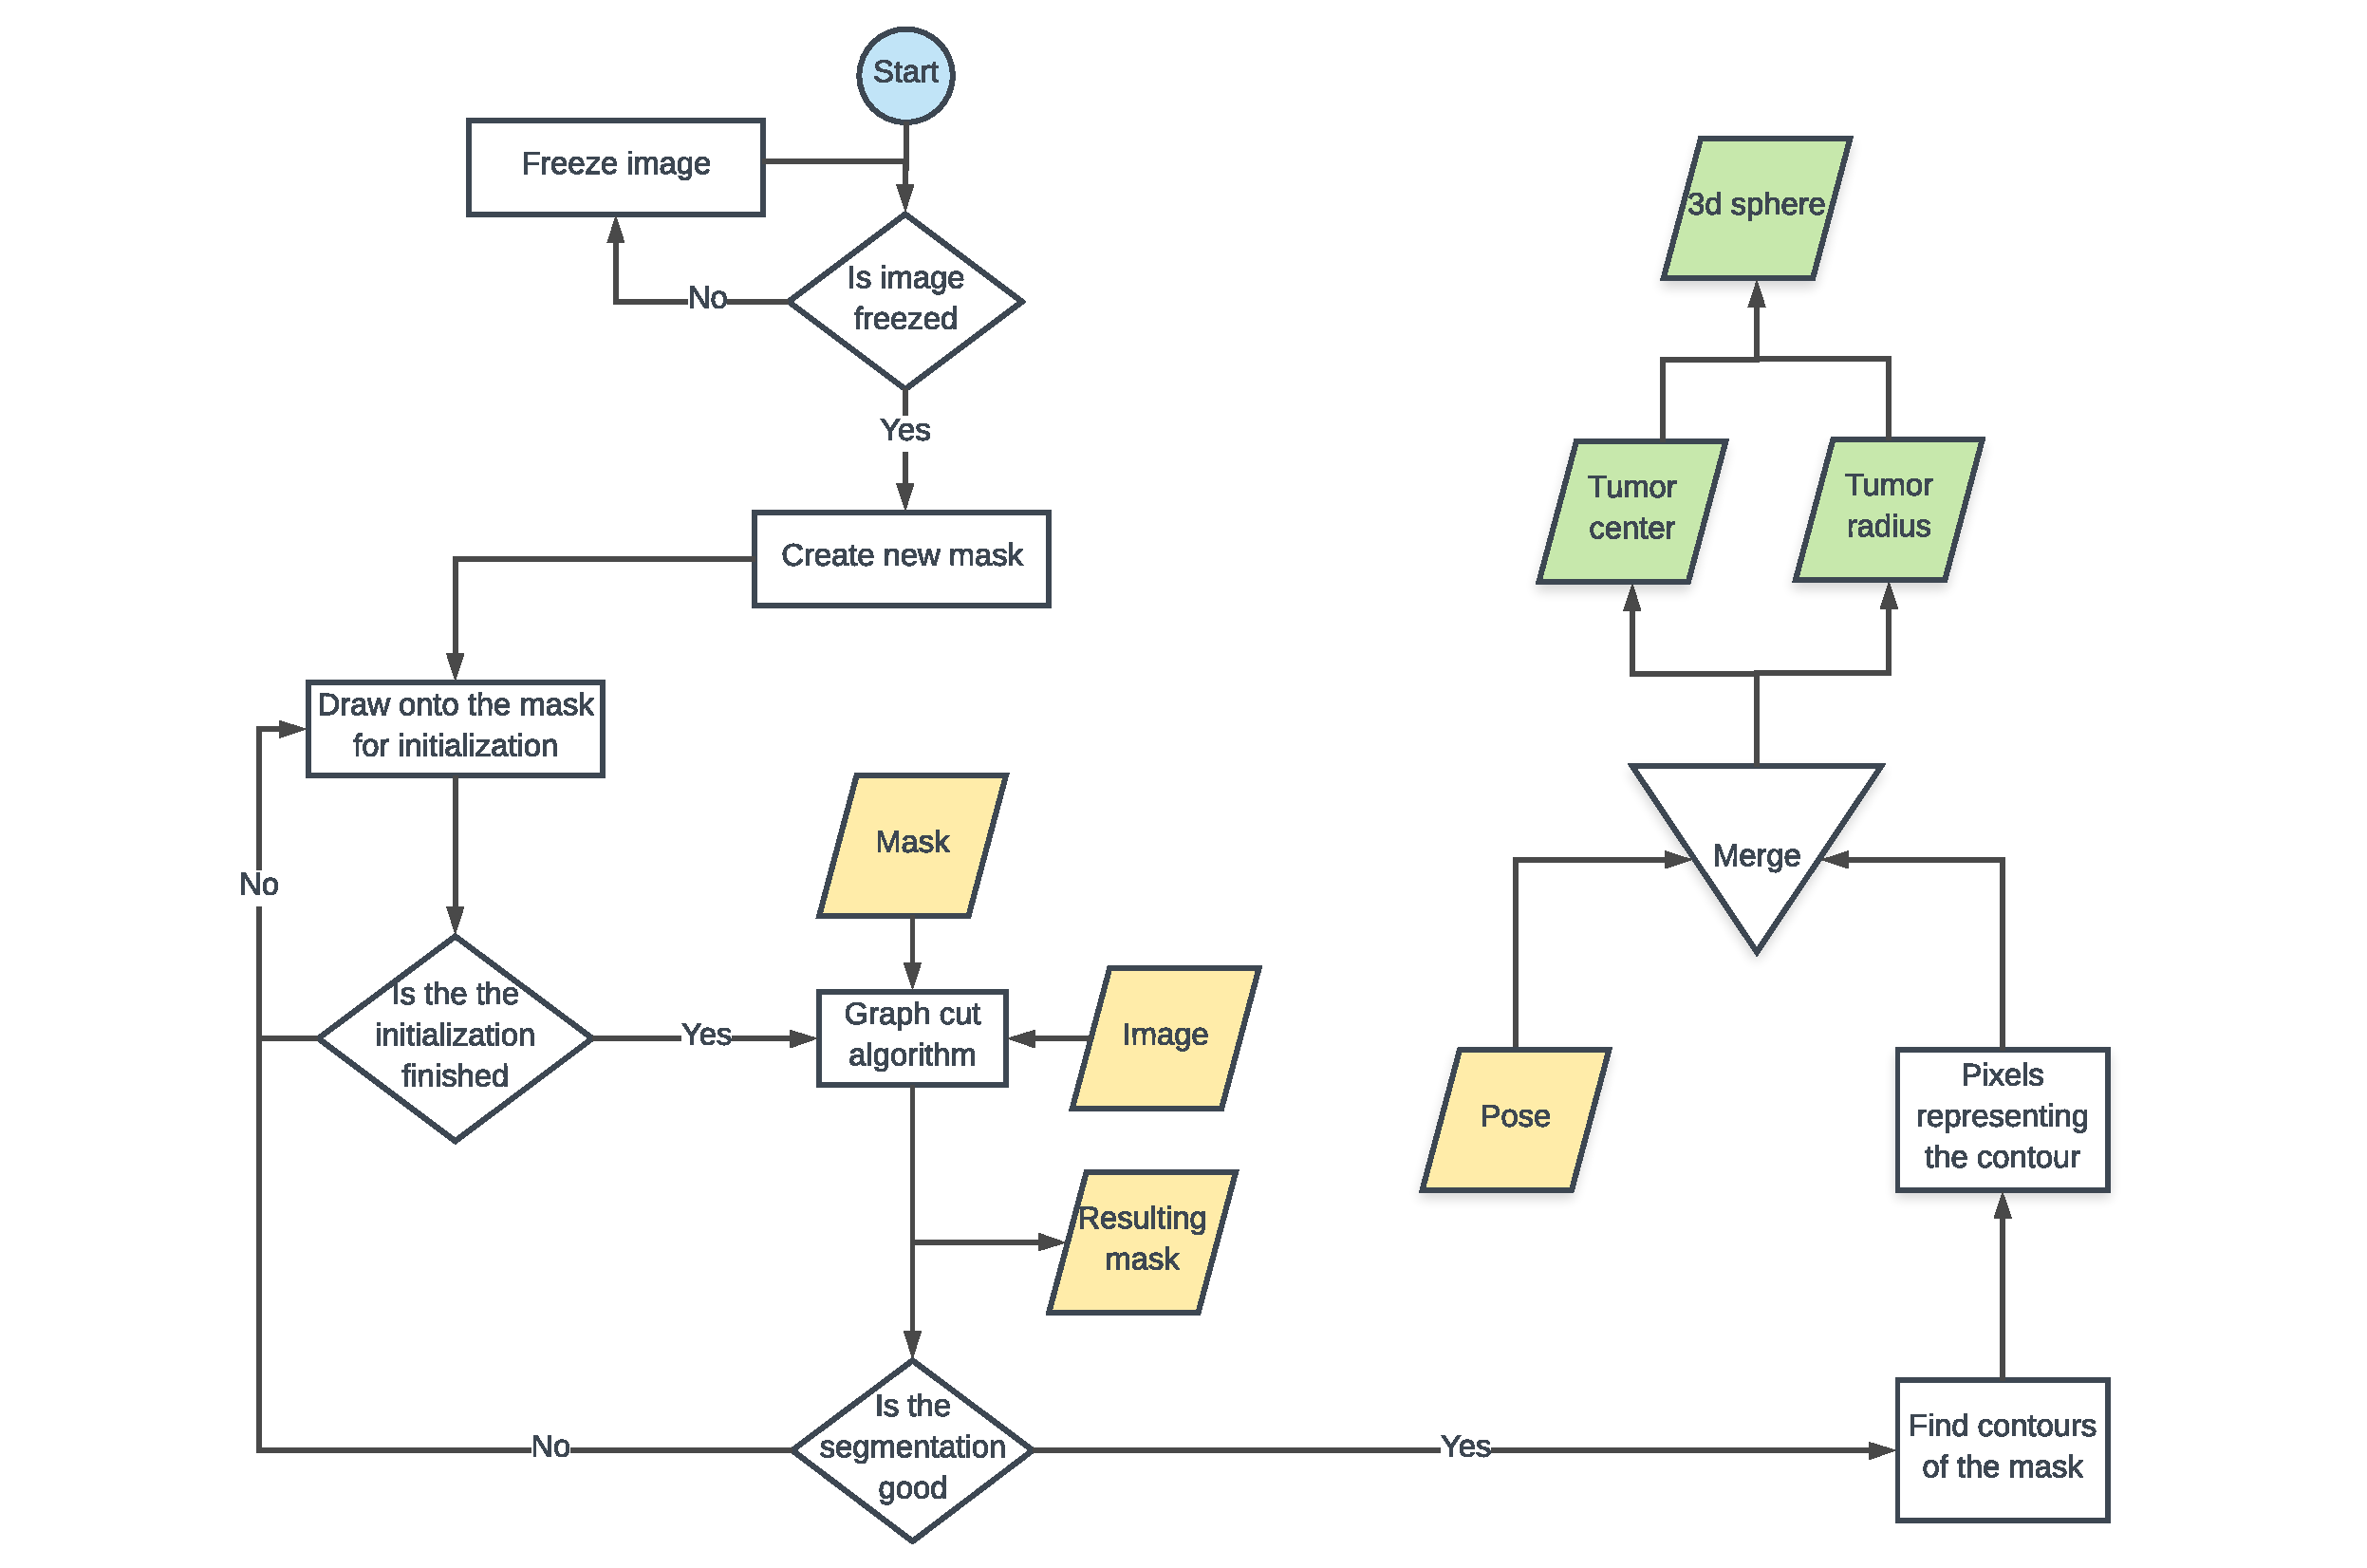
\includegraphics[width=1.2\textwidth]{ThirdFlowChart}
  \caption{The way of the image and its pose if the surgeon is scanning the
    surface.}
  \label{fig:ThirdFlowChart}
\end{figure}

\subsection{Initialization method}
As explained in section \ref{sec:tumorSegmentation}, the segmentation of the
tumor has to be initialized manually. This is done by drawing onto an
initialization mask. The surgeon draws two circles onto the mask. After clicking in the middle of the tumor, two
circles are drawn onto the mask. An orange
circle for the pixels that should be looked at to find the boundary of the
tumor (Figure \ref{fig:InitializeGraphCut}). And a red circle to color pixels surely
originating from the tumor. Most of the time the two circles need to be
increased or decreased in size. This is done by clicking the plus or minus
buttons. Both circles are changed at the same time. The position can be changed
by using the arrow buttons. As soon as the surgeon is satisfied, he confirms the
initialization and the created initialization mask is passed to the segmentation algorithm.
\begin{figure}[H]
  \centering
  \minipage{0.62\linewidth}
  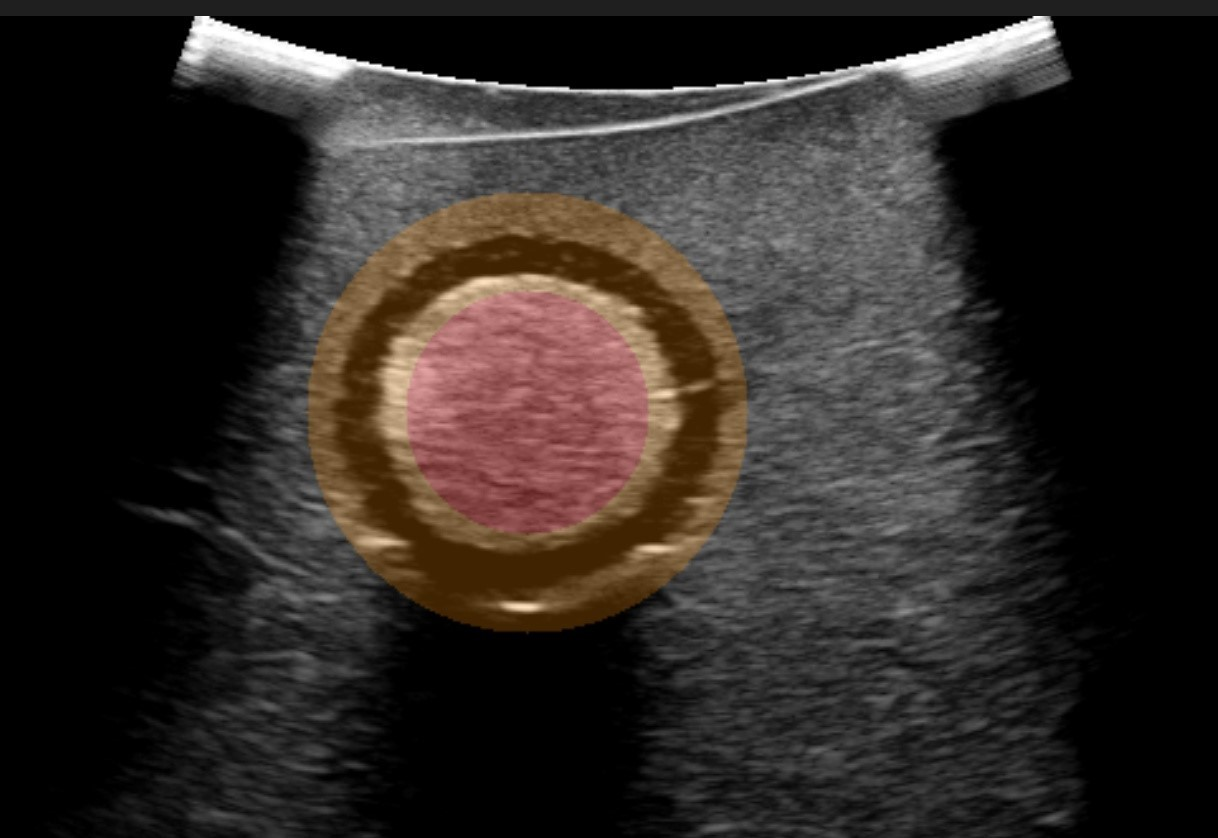
\includegraphics[width=\linewidth]{InitializationDrawing}
  \endminipage
  \hfill
  \minipage{0.32\linewidth}
  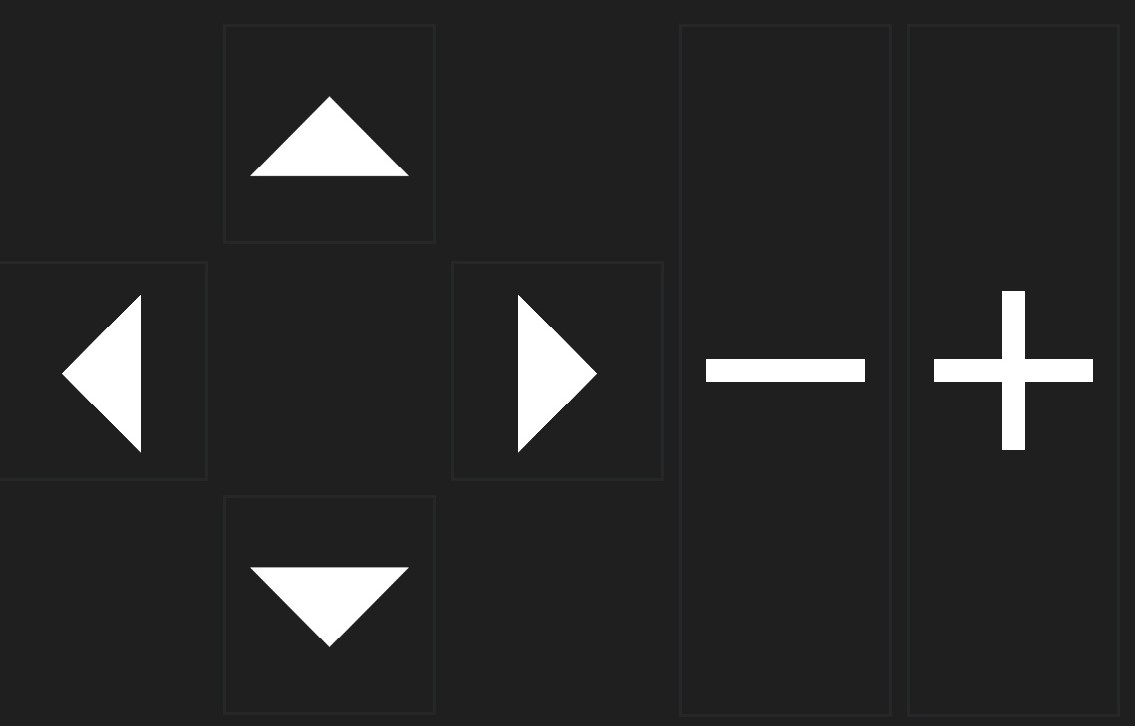
\includegraphics[width=\linewidth]{InitializationControls}
  \endminipage
  \hfill
  \caption{On the left side: Initialization drawing for the segmentation of the
    tumor. Red the pixels which are tumor pixels. And orange the pixels that are
    from the tumor or the background. The not colored pixels represent
    background. On the right side: Controls to manipulate the initial segmentation.}
  \label{fig:InitializeGraphCut}
\end{figure}

\subsection{Graph cuts}
For the segmentation a graph cuts algorithm is used. This algorithm treats
pixels as set of nodes connected in a graph (Figure
\ref{fig:graphCutsExplanaition}). Foreground and background are initialized by
selecting parts in the image.
% Some pixels have to be initialized
% as foreground and background.
Pixels labeled foreground belong to the source and
background labeled ones to the sink. The nodes (pixels) are connected to their
neighbors, the source, and the sink by
edges whose weights are defined as follows:
\begin{itemize}
  \item Node to source $\rightarrow$ Probability of the node to belong to the source (foreground)
  \item Node to sink $\rightarrow$ Probability of the node to belong to the sink (background)
  \item Node to adjacent node $\rightarrow$ Similarity measure to its neighboring node. 
\end{itemize}
A weight of an edge to adjacent node depends on the similarity between pixel intensities.
The edges between adjacent nodes, initialized to the same label, have an
infinitly high weight \cite{wiki:MaxFlow}.

After calculating all the weights in the graph, it has to be cutted in order to
create a segmentation. All pixels not assigned already in advance foreground or background will get assigned by
cutting the graph. The segmentation is obtained in form of a min-cut
\cite{Bagci2016} in which edges are removed to separate source and sink, and sum of their weights is
minimized.
% This means one separates the
% source from the sink by removing edges. All weights of the removed edges have to be summed up.
% The sum should be as small as possible and still separate the two from each
% other.
This way you can find a group of foreground and background pixels.
\begin{figure}[H]
  \centering
  \minipage{0.10\linewidth}
  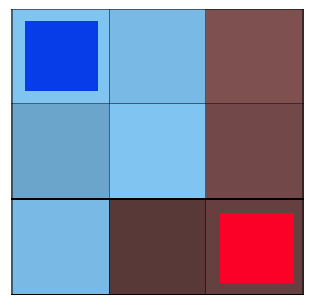
\includegraphics[width=\linewidth]{GraphCuts0} 
  \endminipage
  \hfill
  \minipage{0.22\linewidth}
  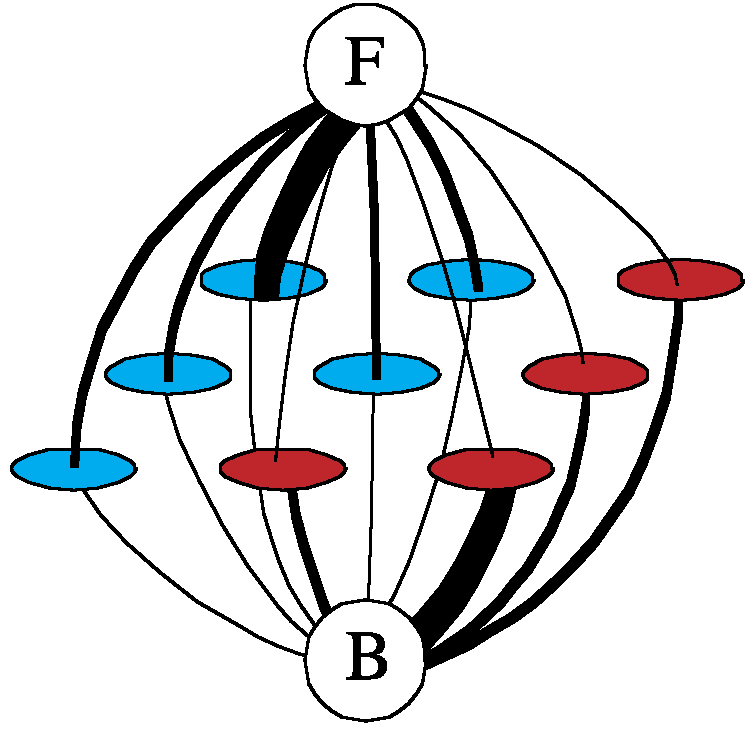
\includegraphics[width=\linewidth]{GraphCuts1} 
  \endminipage
  \hfill 
  \minipage{0.22\linewidth}
  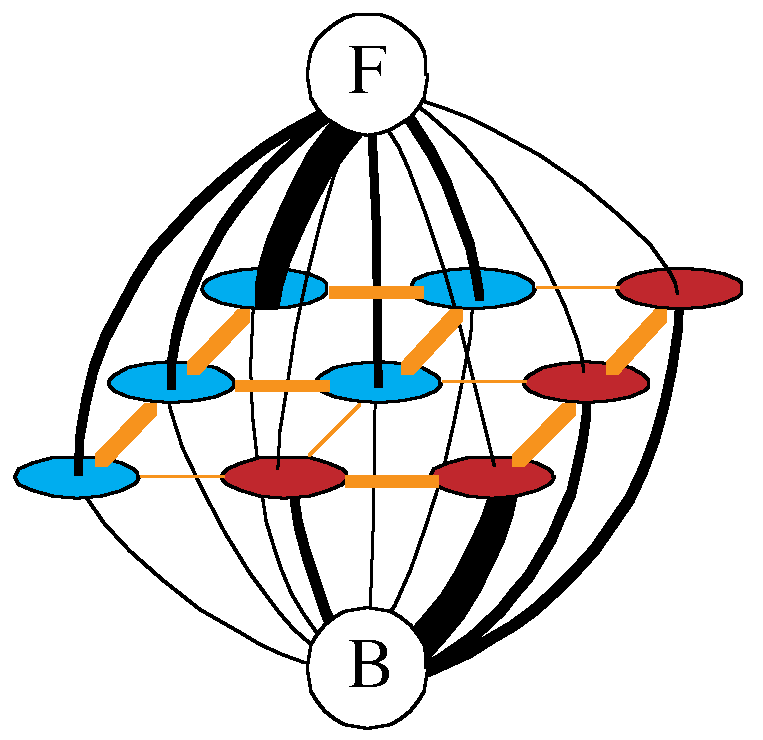
\includegraphics[width=\linewidth]{GraphCuts2} 
  \endminipage
  \hfill
  \minipage{0.22\linewidth}
  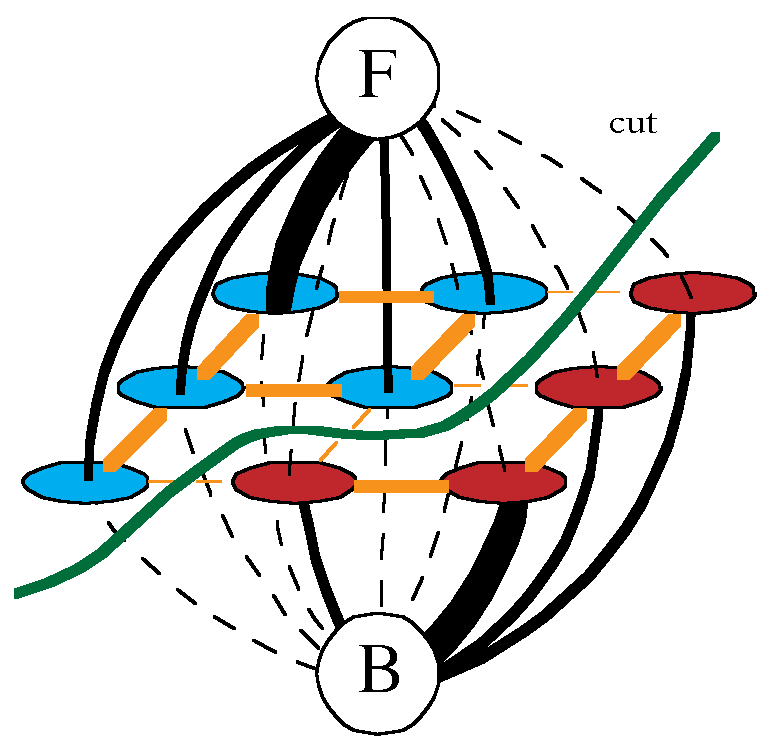
\includegraphics[width=\linewidth]{GraphCuts3} 
  \endminipage
  \hfill
  \minipage{0.22\linewidth}
  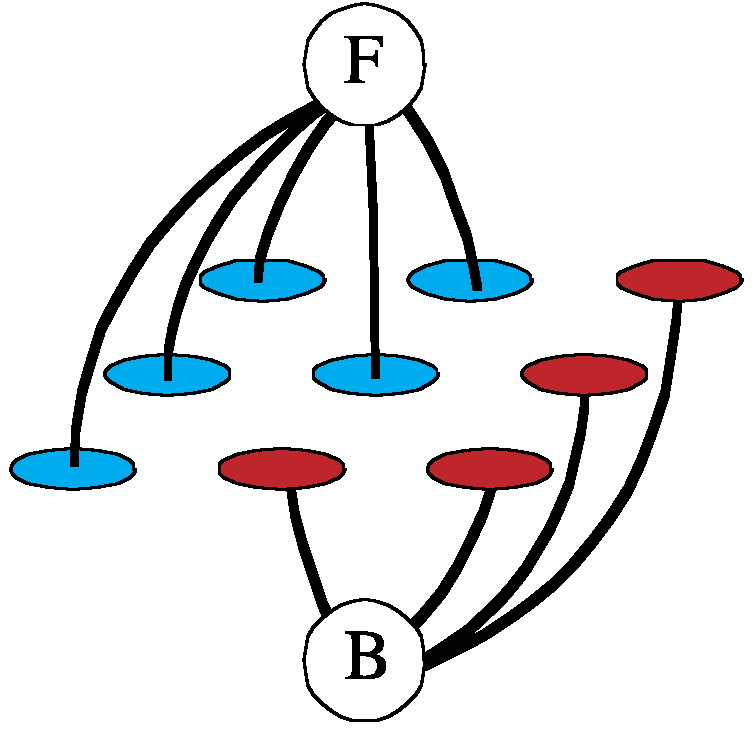
\includegraphics[width=\linewidth]{GraphCuts4} 
  \endminipage
  \hfill
 \caption{From left to right the steps of a graph cut segmentation. The first
   image shows the nine pixels to separate into foreground and background. A
   clear blue and a clear red drawing onto two pixels indicate the initialized
   foreground and background. The
   second image ilustrates the probabilities of each pixel belonging to the
   foreground or the background. The third image shows the edges between
   neighboring pixels in orange. The fourth image shows the edges to be cut as
   dashed lines. Finally the last image shows the result for foreground and
   background \cite{Bagci2016}.}
  \label{fig:graphCutsExplanaition}
\end{figure}

\section{Resection Planning}
The 3D models of the liver and the tumor are created. In this section we will
explain how the resection plane is calculated and displayed in the 3D scene. In
order to make better planning possible, the nearest point to the tumor center on
the surface of the liver must first be determined. To find this point, the
\textit{vtkCellLocator} class is used. This class has a function that can be
used to find the nearest point on a surface to a given point and the distance
between them. The found point and distance together with the polygonal data of
the liver surface, tumor, value for the safety margin, and the desired resection
shape are then passed into the resection calculator (Figure
\ref{fig:FourthFlowChart}).

The resection calculators task is to create a resection plane under the given
conditions and to represent it in the 3D model. It also shows the safety margin taken
into account as a sphere around the tumor. In addition, also a help line is displayed
on the liver surface to show where the surgeon could start the resection.
\begin{figure}[H]
  \centering
 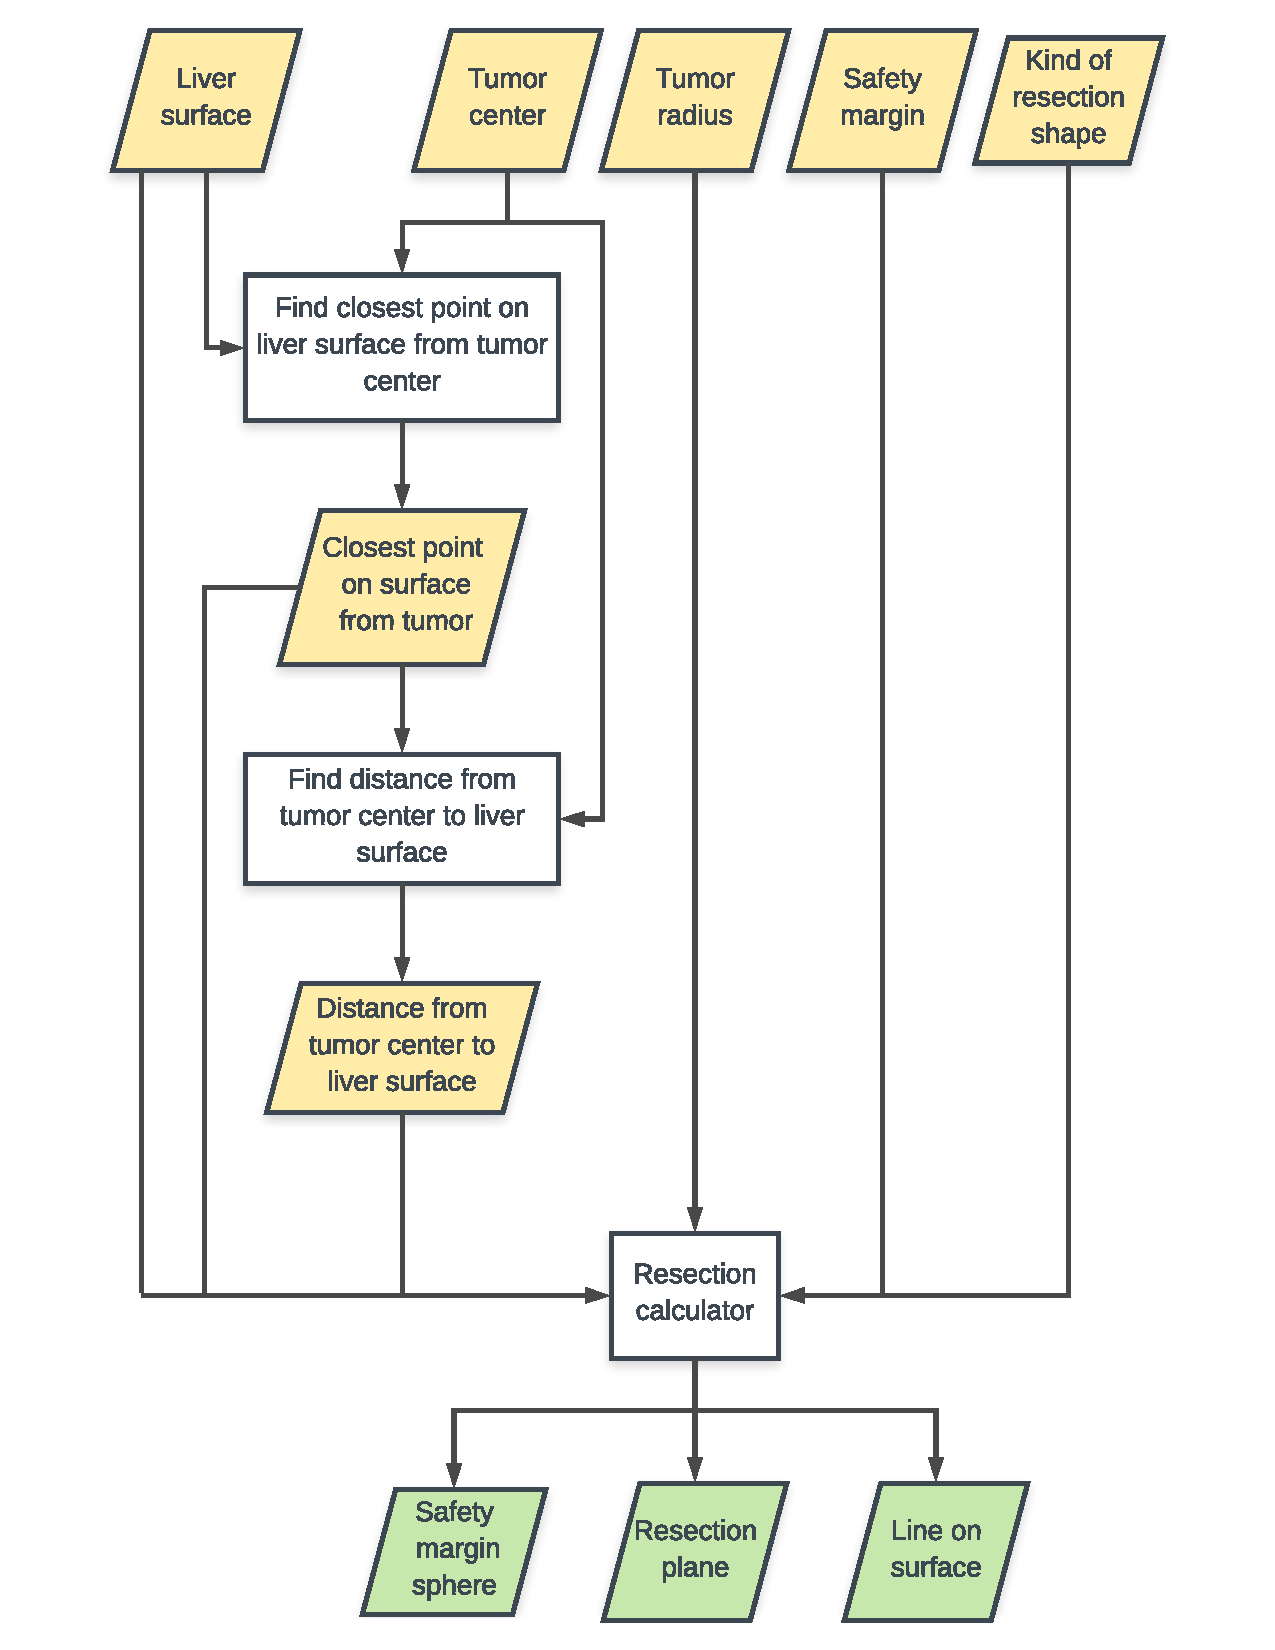
\includegraphics[width=0.65\textwidth]{FourthFlowChart}
  \caption{This flow chart shows the data flow to and from the resection calculator.}
  \label{fig:FourthFlowChart}
\end{figure}

\subsection{Cone fitting around tumor}
In order to keep as much healthy tissue as possible and still remove the tumor
while maintaining the necessary safety margin around the tumor, the resection
plane is recalculated for each tumor. Depending on the distance (d) between tumor
center (C) and liver surface the angle $\alpha$ varies between 10° and 30°. For
tumors with a distance less than 10 mm the angle is fixed to 30° and for
distances larger than 30 mm the angle is fixed to 10°. The direction of the cone
is defined by the vector from the tumor center to the nearest point (P) on the
surface. After constraining the cone to be tangential to the sphere of the
safety margin on both sides, the position of the cone apex (A) can be calculated. By
additiaonally forcing the cutting of the cone tangential to the sphere of the
safety margin, the length of the cone is limited towards the apex. The base of
the cone is defined to be 10 mm further away from the tumor than the surface
point. Finally we have the shape, size and position of the cone that leads to a
tissue sparing resection of the given tumor.
\begin{figure}[H]
  \centering
 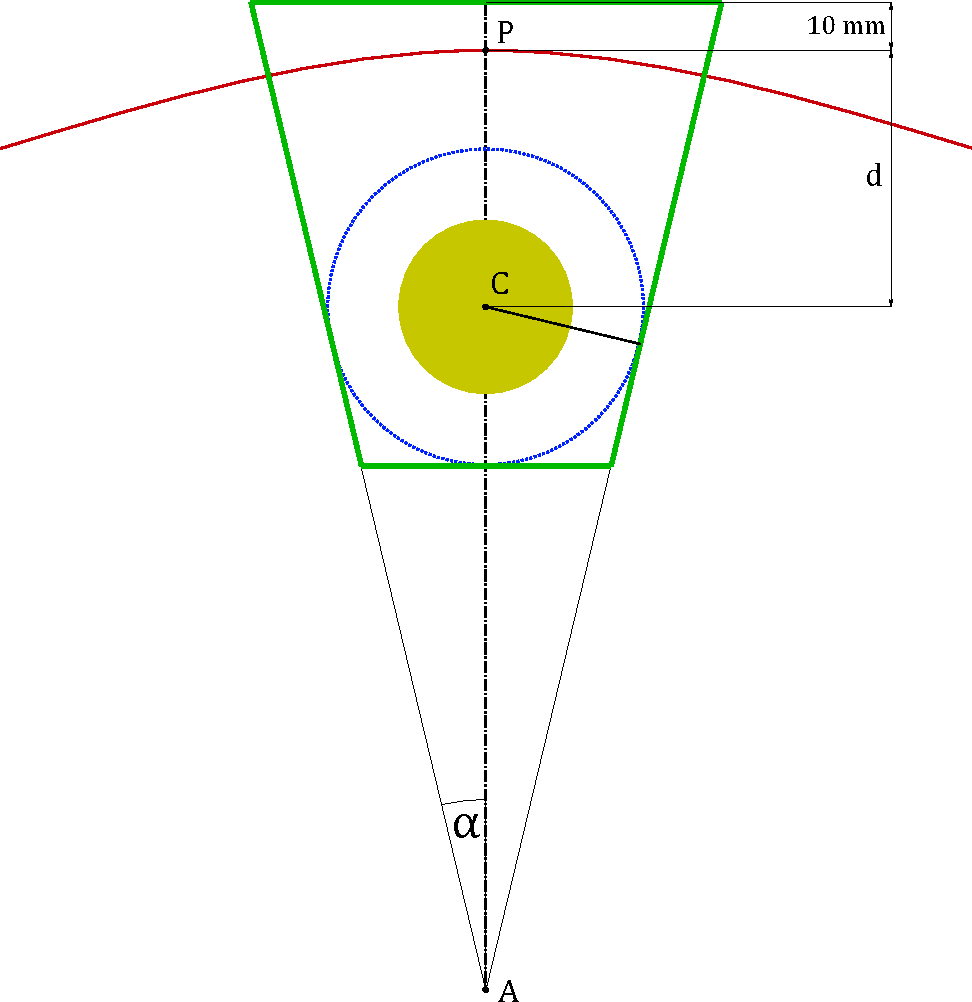
\includegraphics[width=0.5\textwidth]{ConeFittingGeometry}
  \caption{The geometrical shape of the resection plane (green) after fitting it
  around the safety margin (blue). The angle $\alpha$ depends on the distance (d)
  between the tumor center (C) and the closest point (P) on the liver surface to
  it. The position of the apex (A) can be calculated after constraining the
  safety margin to be tangential to the sides of the cone.}
  \label{fig:ConeFittingGeometry}
\end{figure}

\section{Visualization for navigation}
The visualization of the
previously created, virtual, assisting, 3D models to the surgeon should make the intervention
safer or even improve it.
Because surgeons need the ultrasound device a lot during liver resections, it
makes sense to combine the 3D models with the ultrasound image.
% To help the surgeon navigate during the intervention, t
\subsection{Ultrasound overlay}
The ultrasound image ...
\begin{figure}[H]
  \centering
 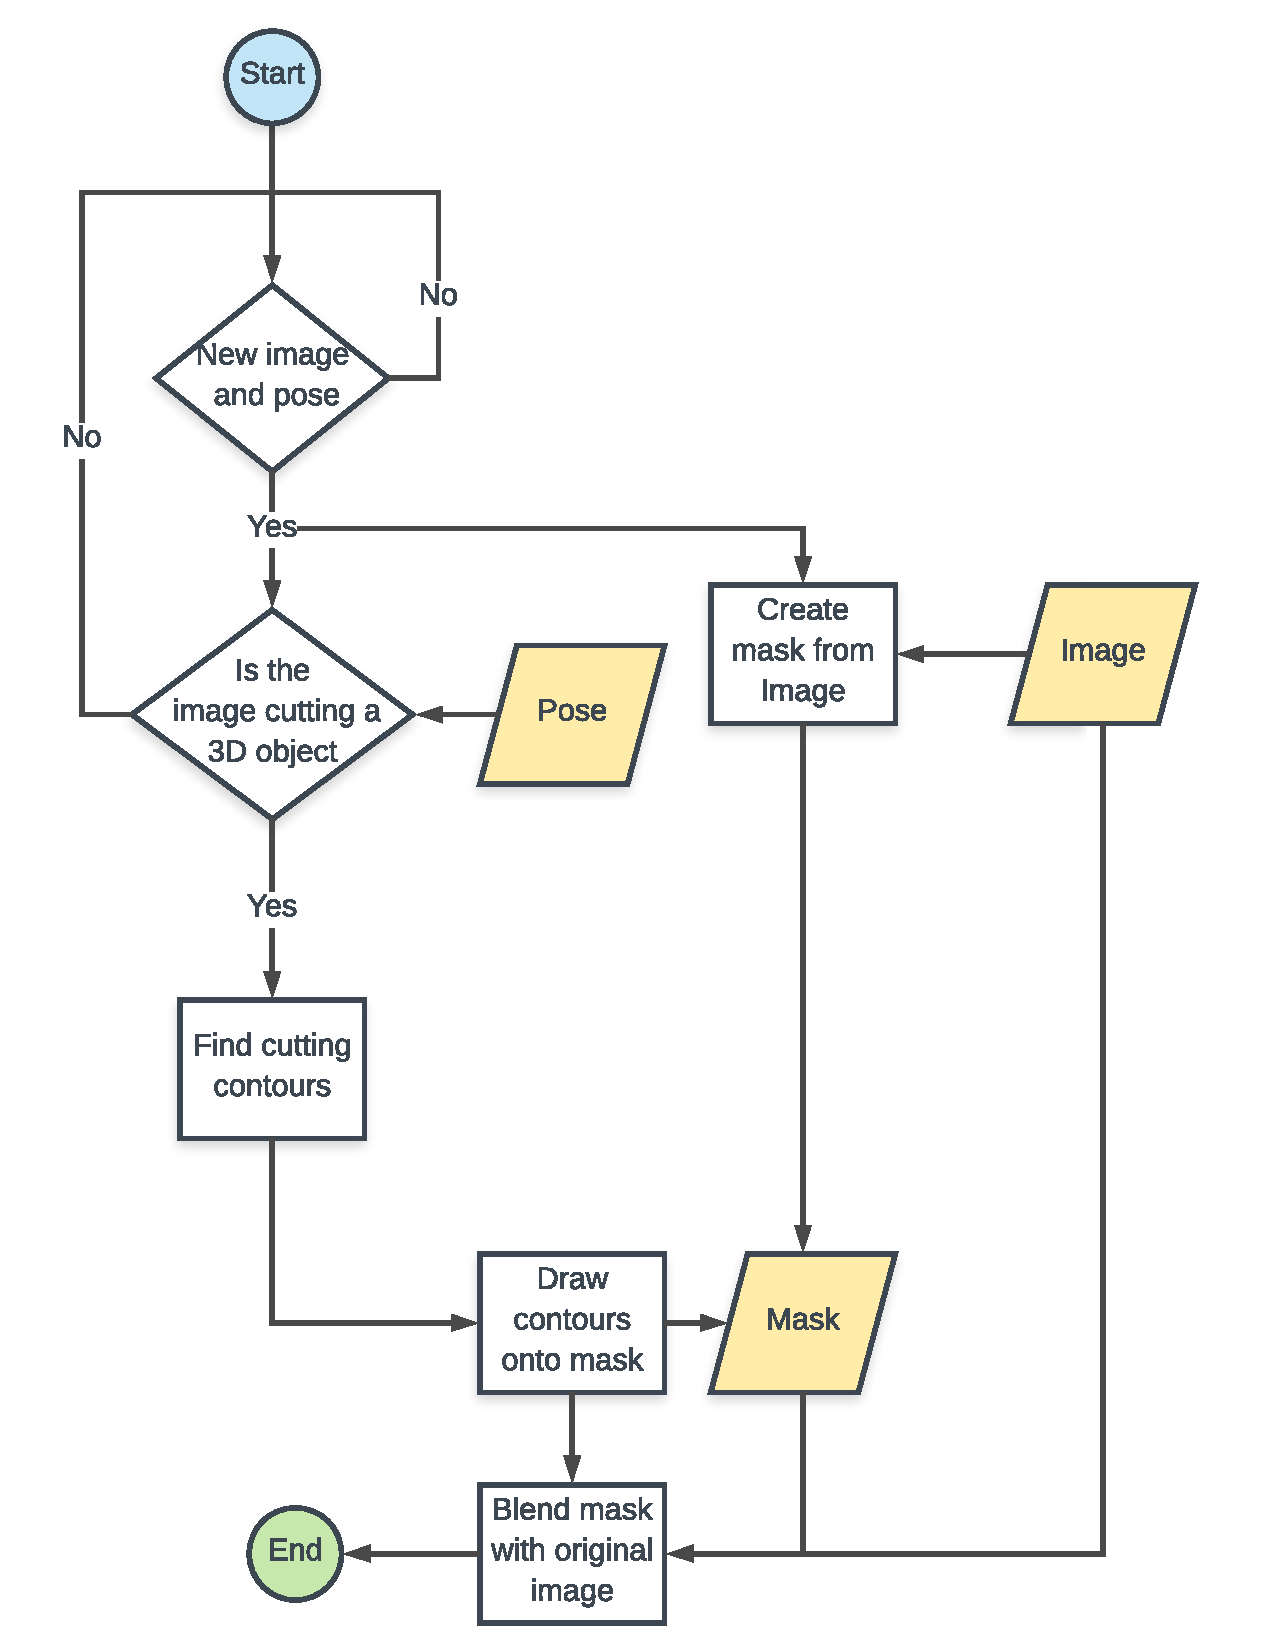
\includegraphics[width=0.5\textwidth]{FifthFlowChart}
  \caption{This flow chart shows the data flow to create the overlay of the 3D
    objects onto the live ultrasound images.}
  \label{fig:FifthFlowChart}
\end{figure}
\begin{figure}[H]
  \centering
  \minipage{0.48\linewidth}
  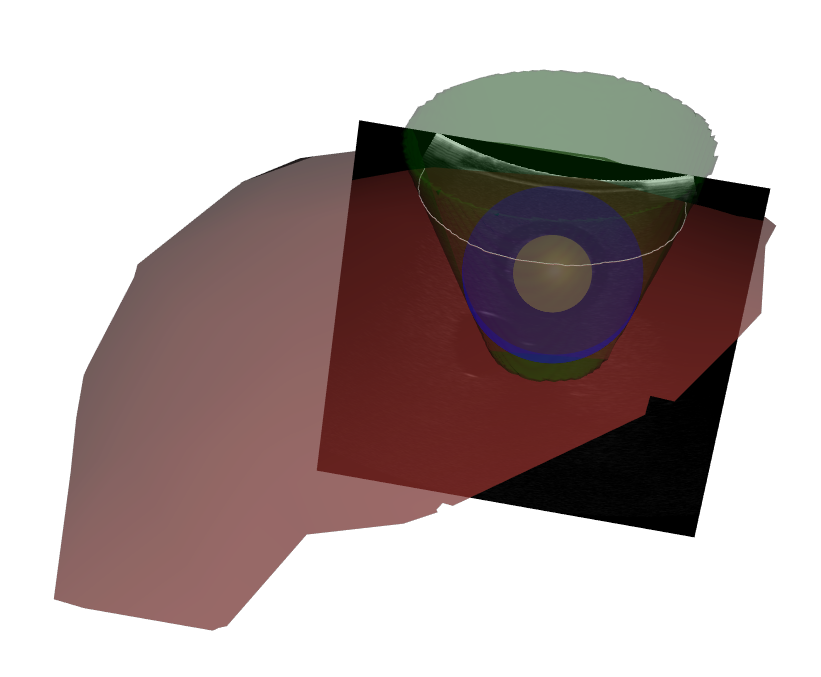
\includegraphics[width=\linewidth]{cutter3DView} 
  \endminipage
  \hfill
  \minipage{0.48\linewidth}
  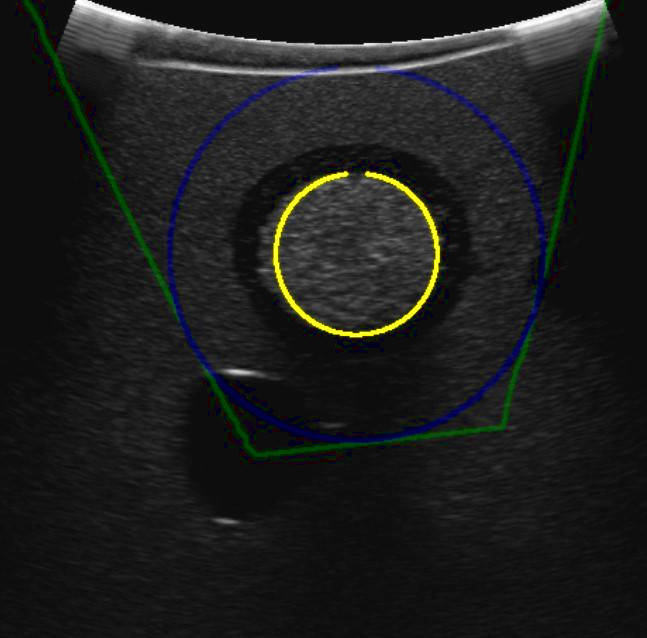
\includegraphics[width=\linewidth]{cutter2DView}
  \endminipage
  \hfill 
 \caption{On the left side is the 3D scene with the ultrasound image cutting
   through the tumor, safety margin and the resection plane. On the right side
   is the resulting cutting overlay on the live ultrasound image.}
  \label{fig:cutterExample}
\end{figure}
\subsection{3D model}
\section{UI Concept}
%%% Local Variables:
%%% TeX-master: "MscThesis"
%%% End:
\chapter{Experiments}
In this chapter .... experiments will be presented. 
\section{Surface Accuracy on a technical phantom}
\label{sec:SurfaceReconstructionAccuracy}
The work presented in this section was presented at CURAC, Luca

Surgical resection is the gold standard for curative care for primary and
secondary hepatic tumors. This procedure usually involves removing the segment
of the liver where the tumor is located. In this treatment, it is important to
spare enough healthy parenchyma to preserve the function of the liver after
surgery. Therefore, non-anatomical resection approaches are becoming more
popular, as they try to spare as much healthy tissue as possible. This way, only
the tumor and a safety margin of 5 – 10 mm are removed which allows multiple
resections and re-treatments in case of recurrence \cite{aghayan2018laparoscopic}.
However, especially in these non-anatomical resections, maintaining the safety
margin is challenging as the tumor is removed by cutting around the tumor in a
conical or wedge shape rather than a plane along anatomical landmarks.
Therefore, image-guidance systems have been introduced to guide the surgeon to
precisely follow a planned resection path. These systems rely on tracking
devices (optical or electromagnetic) to measure the pose of the surgical
instruments and use a registration process to align a preoperative model with
the patient intraoperatively \cite{lango2012navigated}\cite{banz2016intraoperative}. However, the setup and use of such systems
is time consuming, complex and requires extensive training, which is a major
reason why they are not widely used \cite{kingham2013evolution}.
Additionally, the registration process introduces errors due to organ deformation between the image acquisition and the surgery. 
During conventional, non-anatomical resections a resection plan is drawn onto
the liver before the start of the resection. Therefore, an important part of the
resection plan is an accurate reconstruction of the liver surface. This surface
is then used to project the outline of the tumor and a safety margin onto the
surface.
This is where the surgeon would start with the transection of the parenchyma.
Previous work used such surface reconstructions based on laser scanners \cite{simpson2016current} for
intraoperative registration, which requires additional equipment.
In this study, we evaluated an ultrasound (US) based method to automatically reconstruct the liver surface intraoperatively.


\subsection{Methodology}
The image processing pipeline consists of three steps, the acquisition, the
contact detection and the surface reconstruction (Figure \ref{fig:processingPipeline}). First the data from an
ultrasound scanner (Flex focus 800, BK Medical, Denmark) and a tracking camera
(Polaris, NDI, Canada) is acquired and fused on a navigation system (CAS-One
Vario, CAScination AG, Switzerland) for liver surgery. Then each image is
classified whether it has contact to the liver surface or not. The position of
the images with contact to the liver surface are then further processed in the
surface reconstruction step to create a model of the liver surface. The result
is then visualized in a 3D viewer.
\begin{figure}[H]
  \centering
  \smartdiagram[sequence diagram]{Acquisition, Surface contact detection, Surface reconstruction}
  \caption{The data processing pipeline}
  \label{fig:processingPipeline}
\end{figure}

\subsubsection{Acquisition}
During the data acquisition phase, the ultrasound image and the corresponding 6D
pose are recorded using the navigation system. The ultrasound was calibrated
using a Z-wire phantom \cite{peterhans2010fully} and is tracked by an optical tracking system. To
simulate a liver surgery, a multimodal liver phantom (Figure \ref{fig:usedPhantom}) and an
intraoperative ultrasound was used to get the ultrasound images. During the
simulation the ultrasound device had a trackable and calibrated marker attached.
To find an optimal sampling method, the liver was scanned with six different
techniques (Figure \ref{fig:movements}). The two spiral techniques represent recordings
of moving the US device to draw a spiral onto the liver. Either from the center
to the peripheral part (spiral out) or vice versa (spiral in). The two sweep
techniques represent recordings of moving the US device left and right (Sweep
LR) or forward and backward (Sweep FB). The flower technique represents a
recording of moving the US-device to draw a flower onto the liver.
Additionally, a point grid was acquired as reference points for evaluation of
the other reconstructions.

\begin{figure}[H]
  \centering
 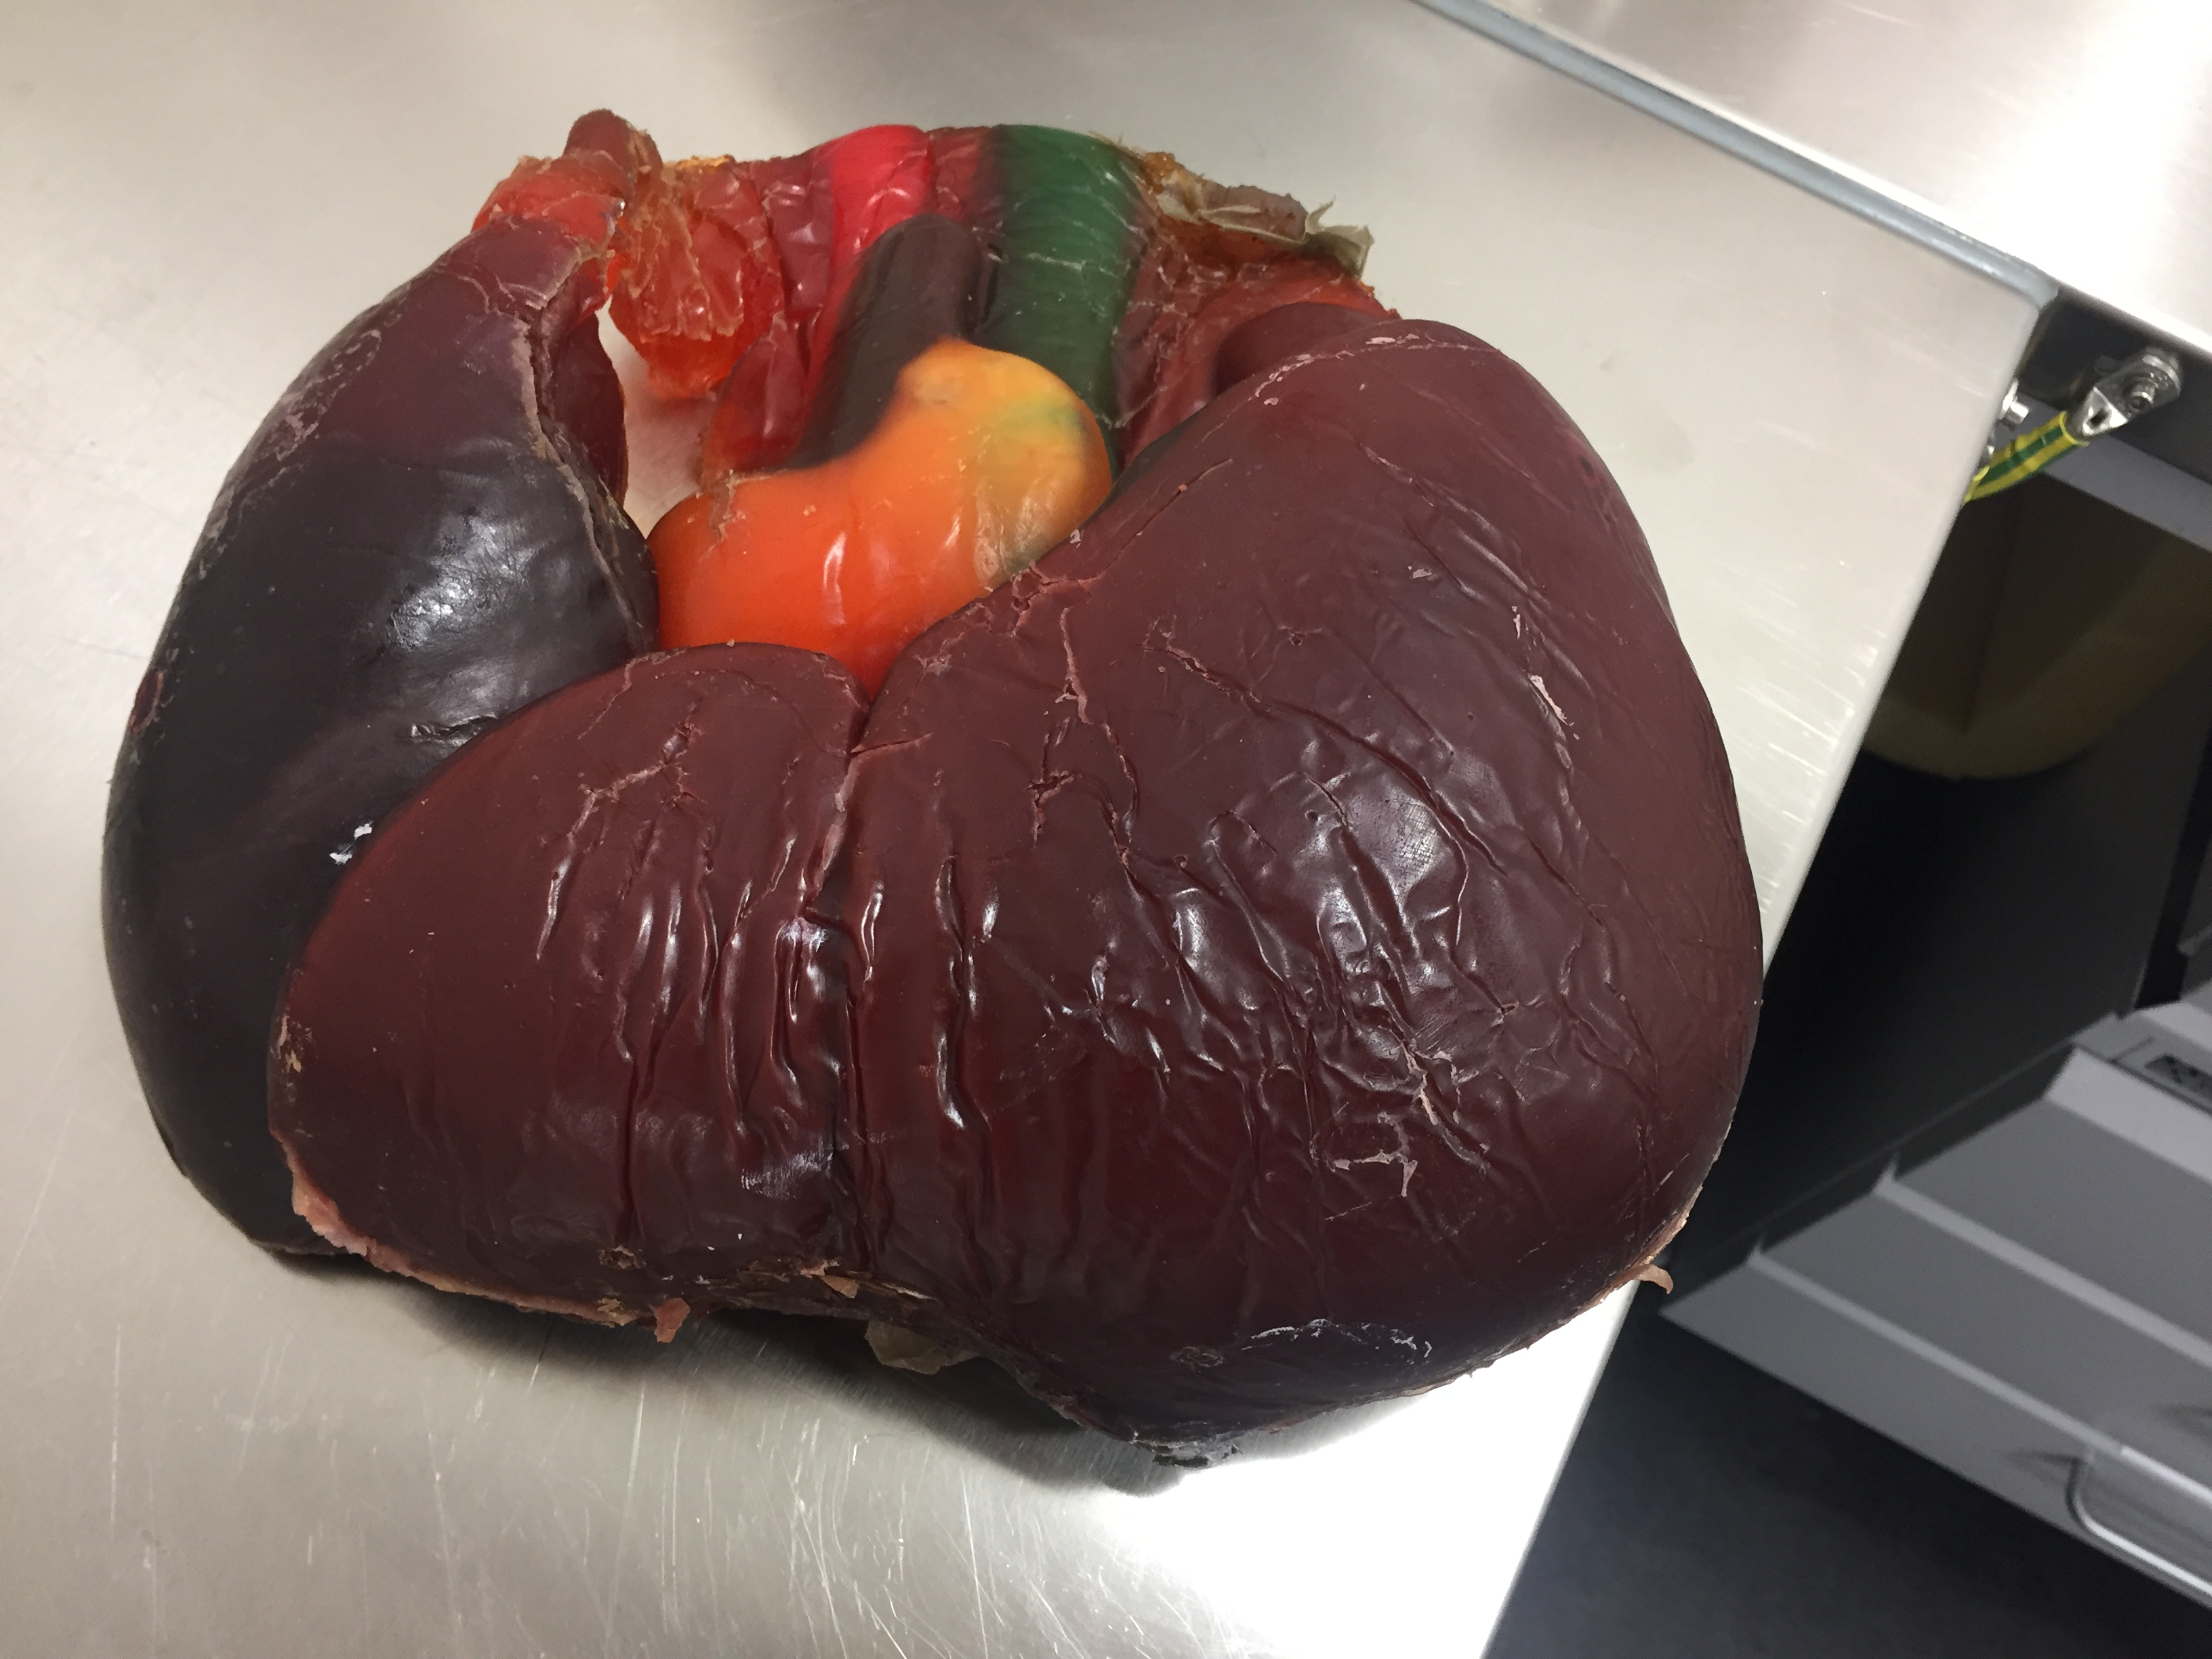
\includegraphics[width=\textwidth]{usedPhantom}
 \caption{The US liver phantom used for the experiments in this study}
  \label{fig:usedPhantom}
\end{figure}

\begin{figure}[H]
  \centering
  \begin{tabular}[H]{c|c|c}
    \addheight{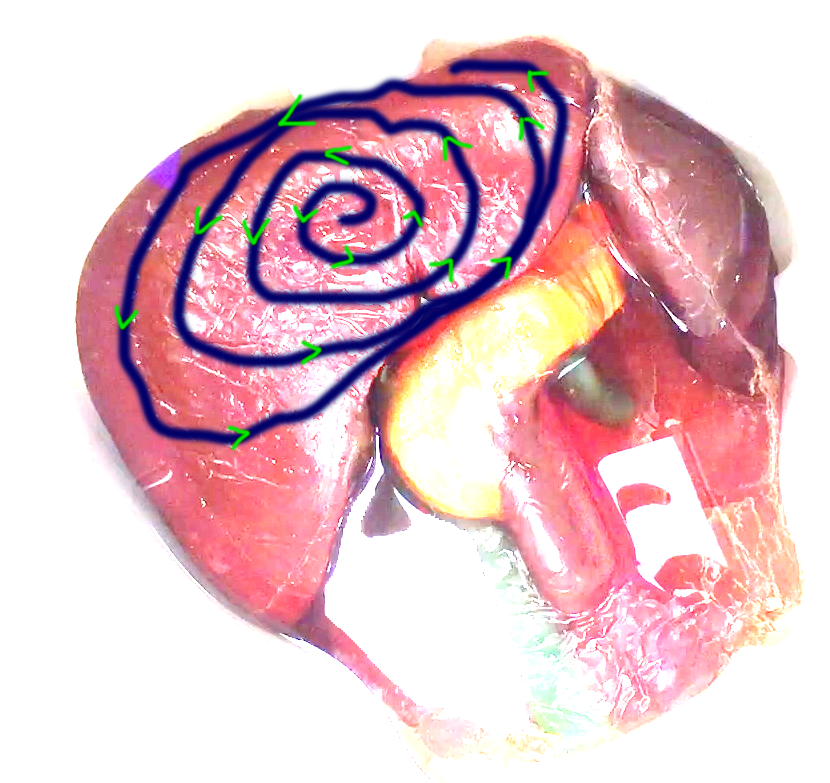
\includegraphics[width=0.3\linewidth]{methods_schnecke_nach_aussen}} &
    \addheight{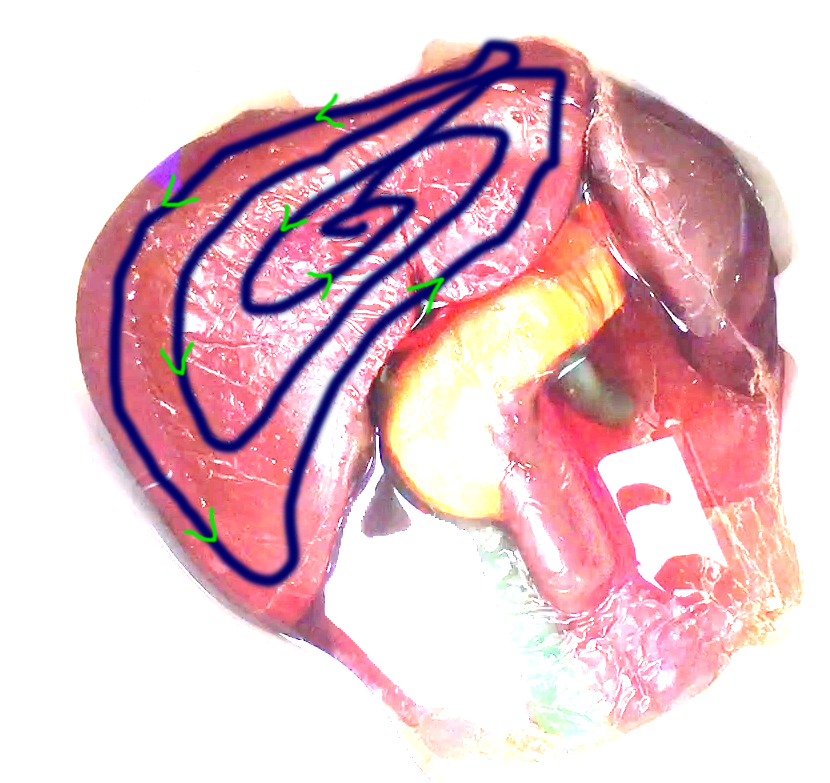
\includegraphics[width=0.3\linewidth]{methods_schnecke_nach_innen}} &
    \addheight{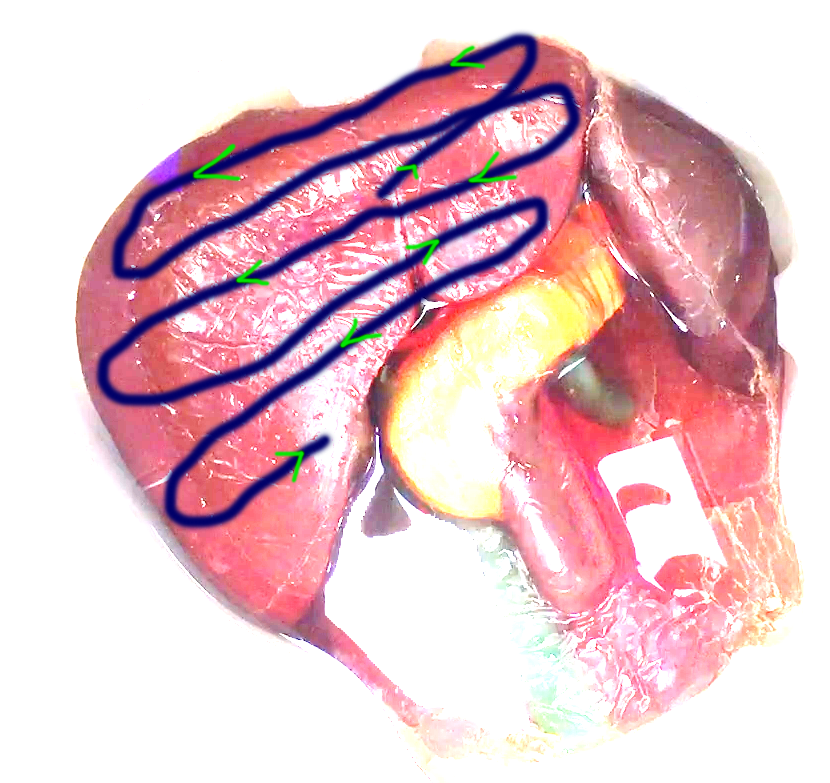
\includegraphics[width=0.3\linewidth]{methods_hin_und_her}}
    \\
    \small Spiral out & Spiral in & Sweep LR
    \\
    \hline
    \addheight{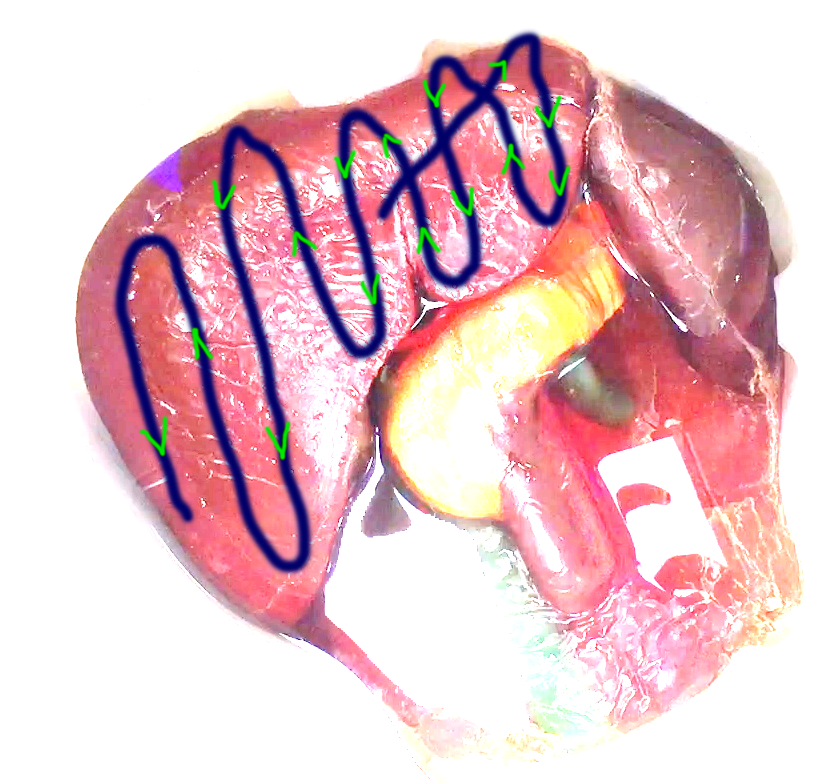
\includegraphics[width=0.3\linewidth]{methods_vor_zurueck}} & 
    \addheight{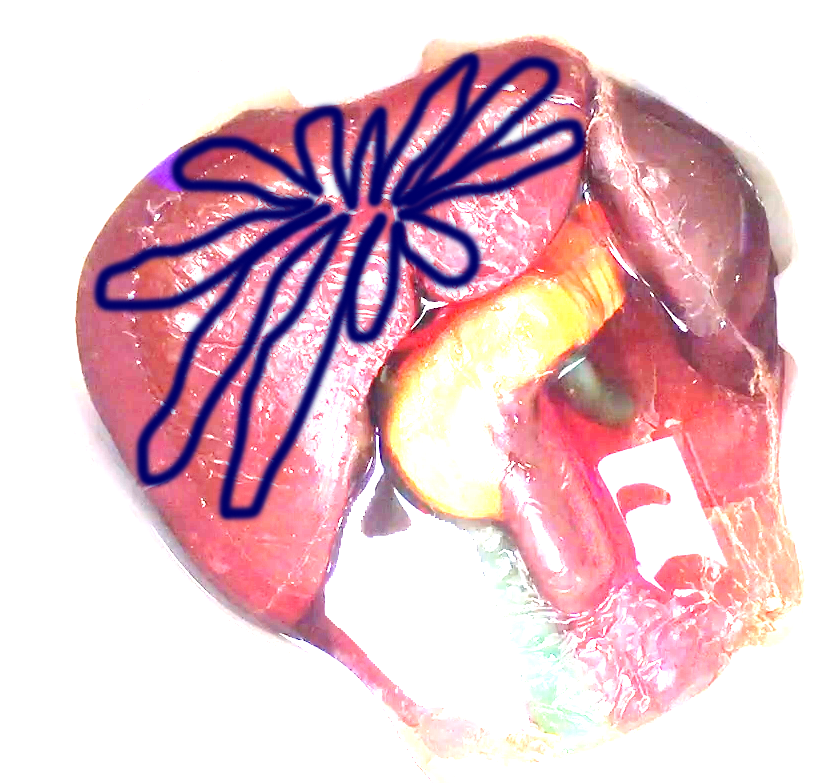
\includegraphics[width=0.3\linewidth]{methods_blume}} &
    \addheight{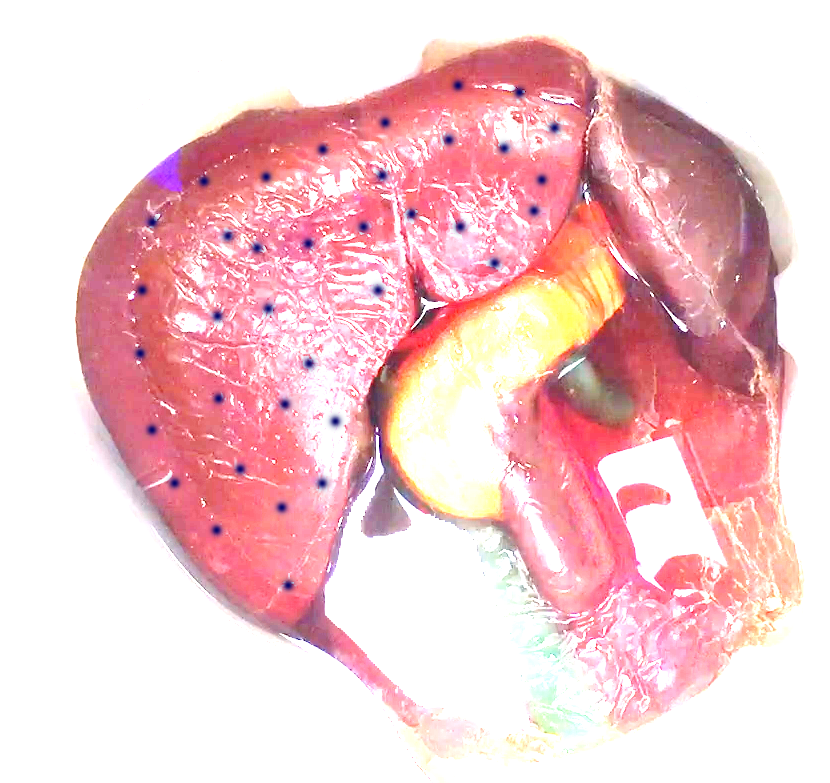
\includegraphics[width=0.3\linewidth]{methods_biene}}
    \\
    \small Sweep FB & Flower & Point grid
    \\
  \end{tabular}
  \caption{Different sampling movements of the ultrasound device over the surface of the liver}
  \label{fig:movements}
\end{figure}

\subsubsection{Surface contact detection}
In the surface contact detection step, a classifier detects whether the US probe
has contact to the liver or not. Therefore, a support vector machine (SVM) was
trained with US images from the phantom and from previous navigated liver
surgeries. The SVM was trained to classify the image into “no surface contact”
(left) and “surface contact” (middle and right). The images were labelled as
“surface contact” if at least 50\% and the center had contact to the surface
(Figure \ref{fig:contactVSnocontact}  middle).  The classifier takes into account that US waves are reflected
at the US probe-air interface when the US probe has no contact to the liver and
therefore no image is formed.
The features for the classifier were: mean, median, minimum, maximum, variance,
skewness and kurtosis of the pixel values. All features are calculated on the
upper half of the image. For training, a set of 2’311 images (1’056 with
contact, 1’255 without contact) were used. The training data was composed of
images from a phantom (88\%) and images from previous navigated liver surgeries
(12\%). All computations were performed using the SciPy software package.


\subsubsection{Surface reconstruction}
To reconstruct the surface of the liver from the sampled points, the surface
reconstruction algorithm by Hoppe et al. \cite{hoppe1992surface}  was used. The algorithm consists
of three phases. From an unorganized set of points, phase 1 constructs an
initial dense mesh. Starting with the dense mesh created in phase 1, phase 2
reduces the number of faces and improves the fit to the data points. In phase 3,
the surface representation is changed from a piecewise linear one (meshes) to a
piecewise smooth one. For the computations the implementation in VTK
(SurfaceReconstructionFilter) was used (neighborhood size of 50 and sample
spacing of 10). Due to the different latencies of the US and the tracking system
(with the US being slower), a delay of 4 frames (0.2 seconds) is applied to the
tracking data.

\subsubsection{Experimental evaluation}
For evaluation of the surface detector the data was split into training (80\%)
and test data (20\%). The precision and recall were calculated for performance
analysis on the test set. To quantitatively evaluate the reconstructed surfaces,
the points of the point grid measurement (414 points) were used as a reference.
These reference points represent points on the surface of the liver in an
undeformed state. For each of these reference points, the error is computed as
the shortest distance to the reconstructed surface. All computations were
performed using SciPy.

\subsection{Results}
Overall, the surface contact detector was evaluated on a test set with 2414
images. Additionally, 10 scans of the liver surface were evaluated against the
reference points to measure the accuracy of the surface reconstruction.

\subsubsection{Surface contact detection}
To evaluate the contact detector, a test set of 2414 images with 50\% contact
and 50\% no contact was used. The detector has a sensitivity of 0.95 and a
specificity of 0.98. Out of all negative samples, 1.9\% were detected as having
contact. The prediction of one image takes 15 ms where most of the time (approx.
99\%) is spent for feature extraction.

\subsubsection{Surface reconstruction}
\textbf{Visual assessment}

The reconstruction of the liver surface created lead to a smoothed version of
the measured surface part. The measured surface corresponds to the surface of
the liver (Figure \ref{fig:usedPhantom}). However, the reconstructed surface area is larger than the
sampled part of the surface. This is a property of the algorithm, as it
estimates a rectangular grid.
\begin{figure}[H]
  \centering
  \begin{tabular}[H]{c|c|c}
    \addheight{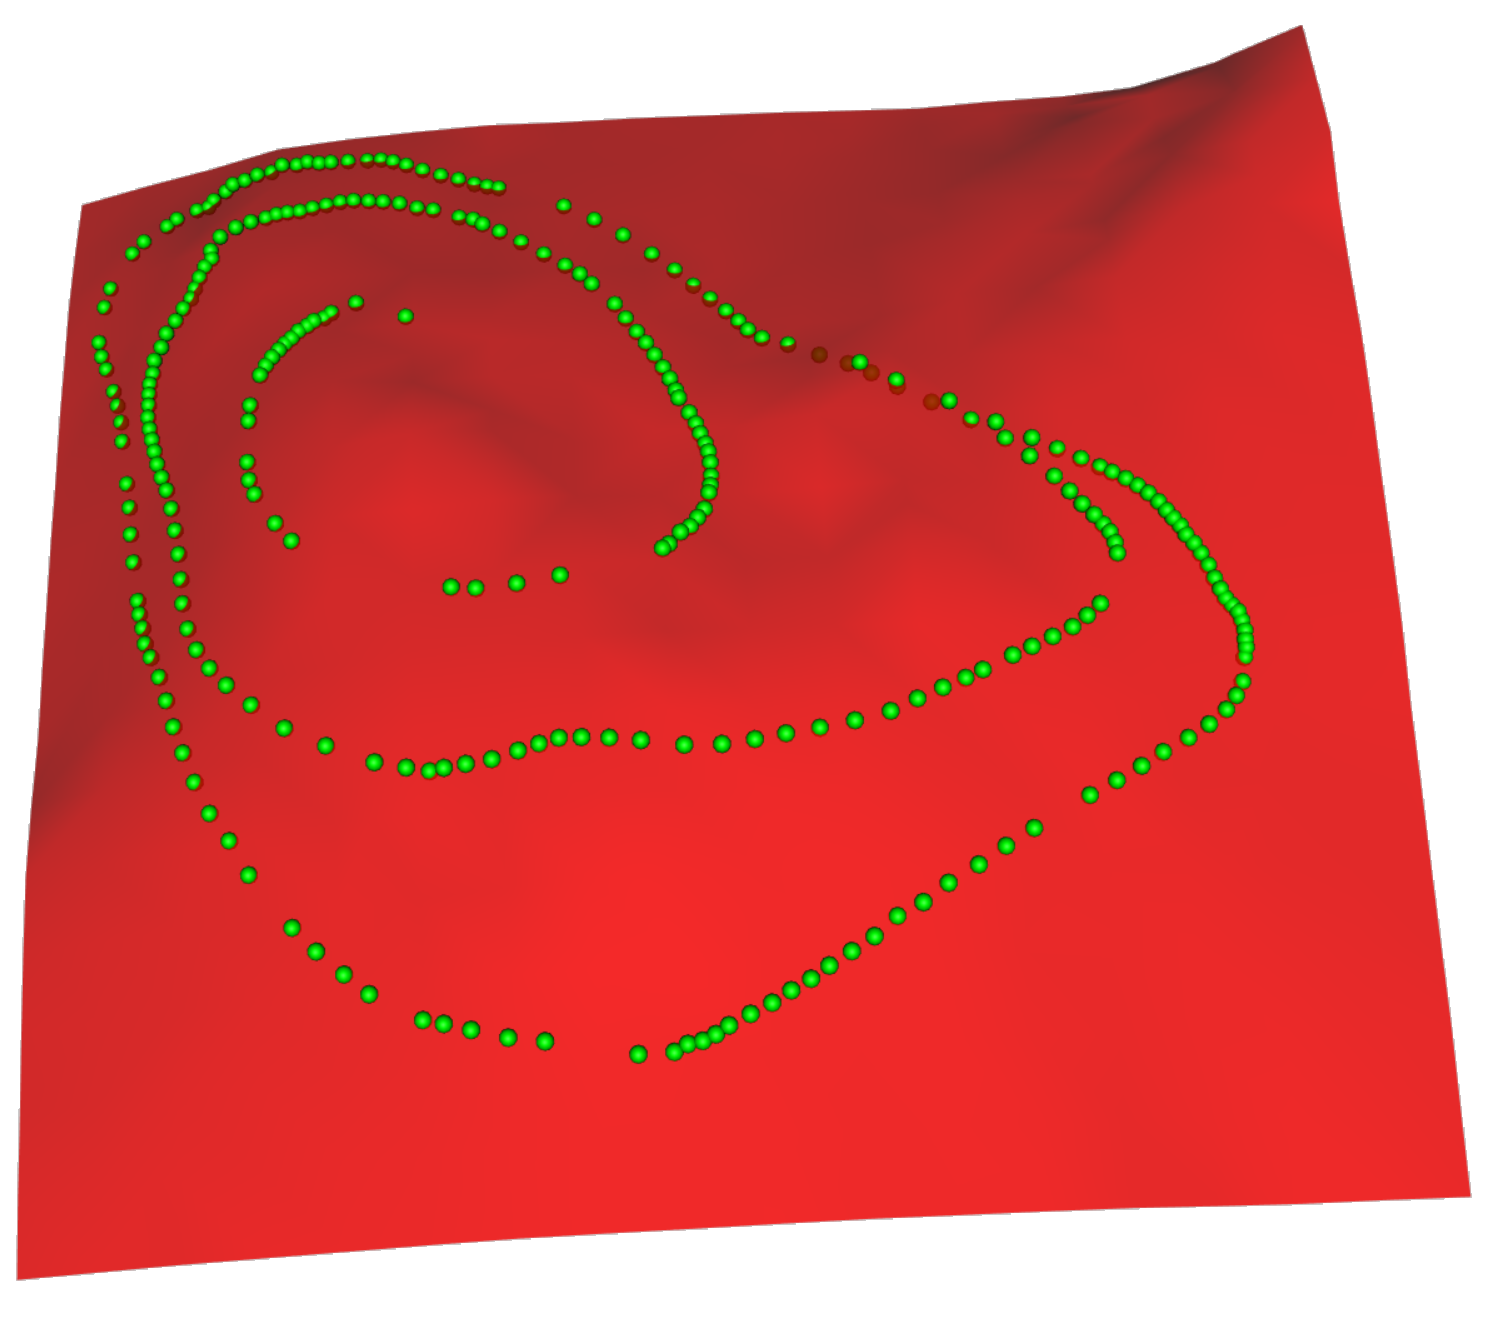
\includegraphics[width=0.3\linewidth]{mes05_spiral_out.png}} &
    \addheight{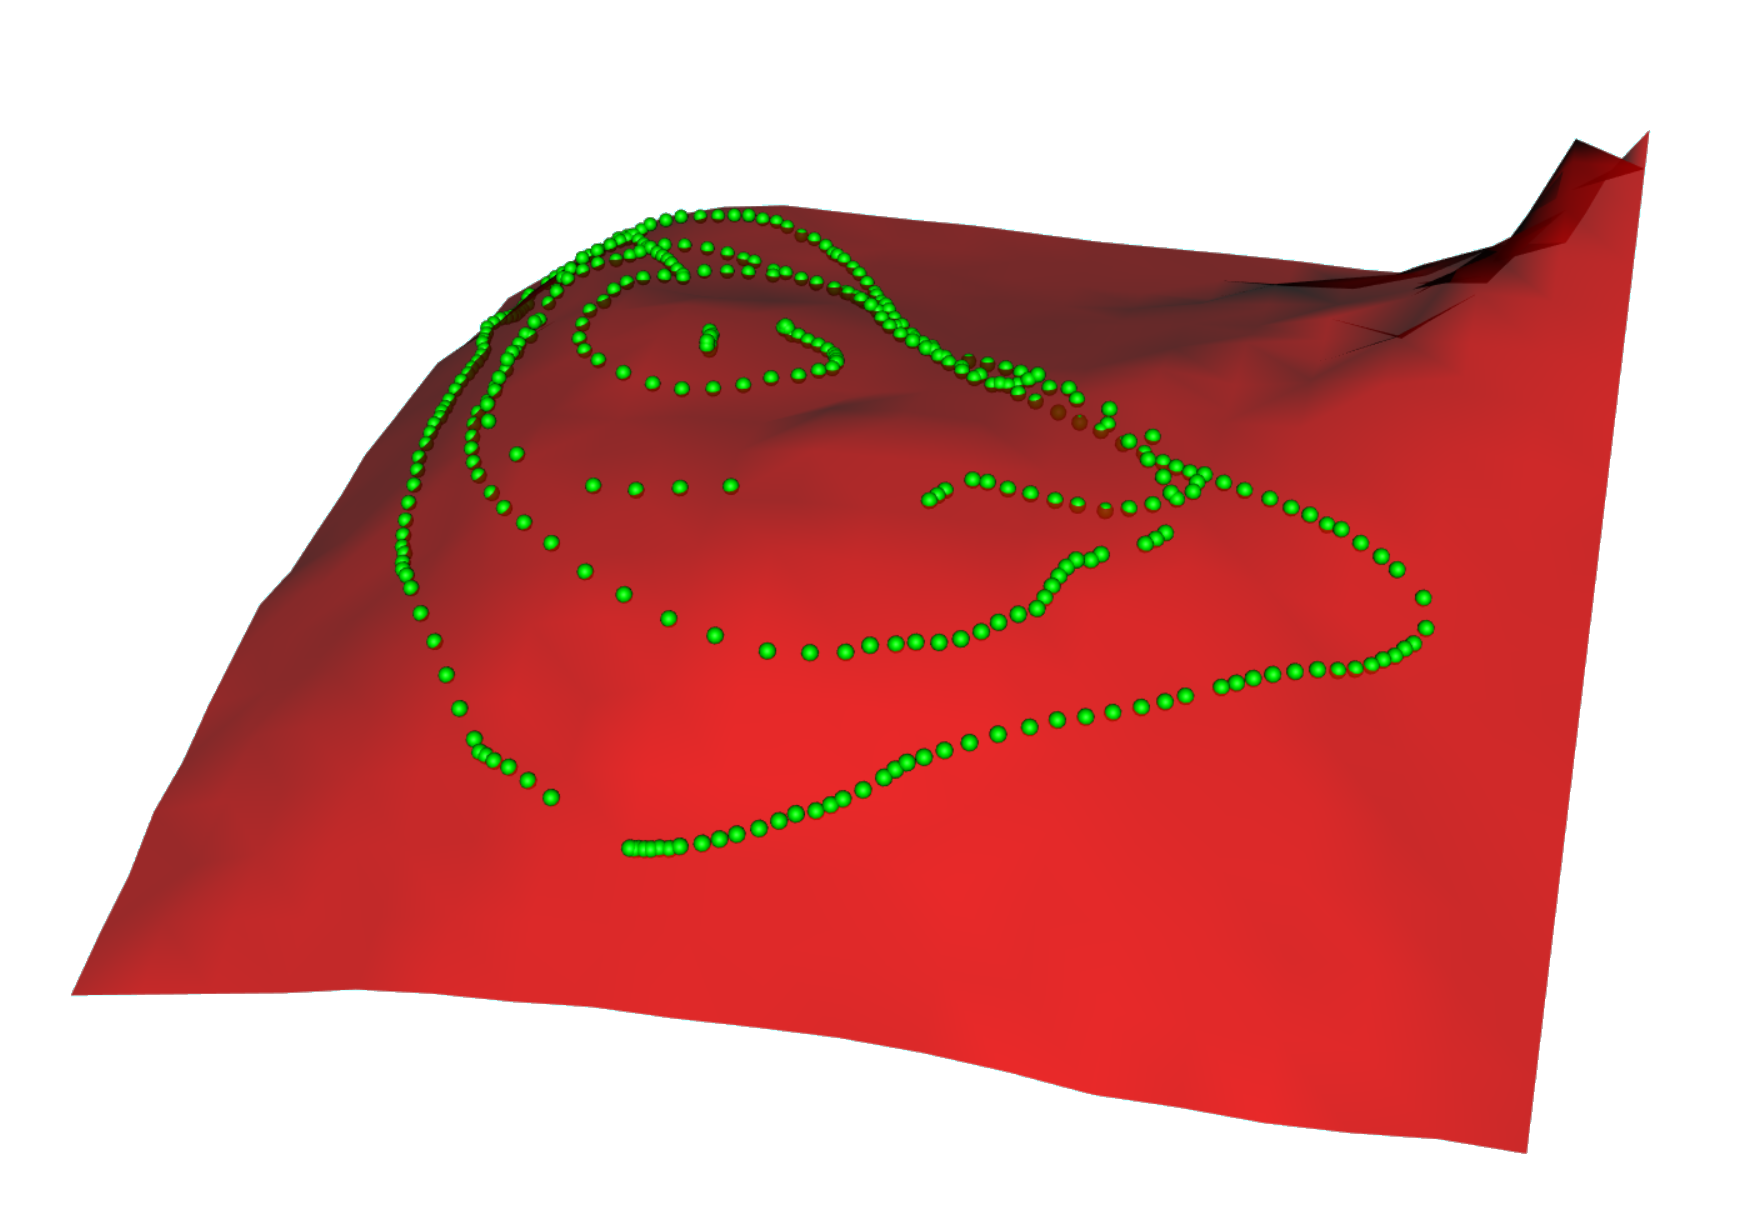
\includegraphics[width=0.3\linewidth]{mes03_spiral_in.png}} &
    \addheight{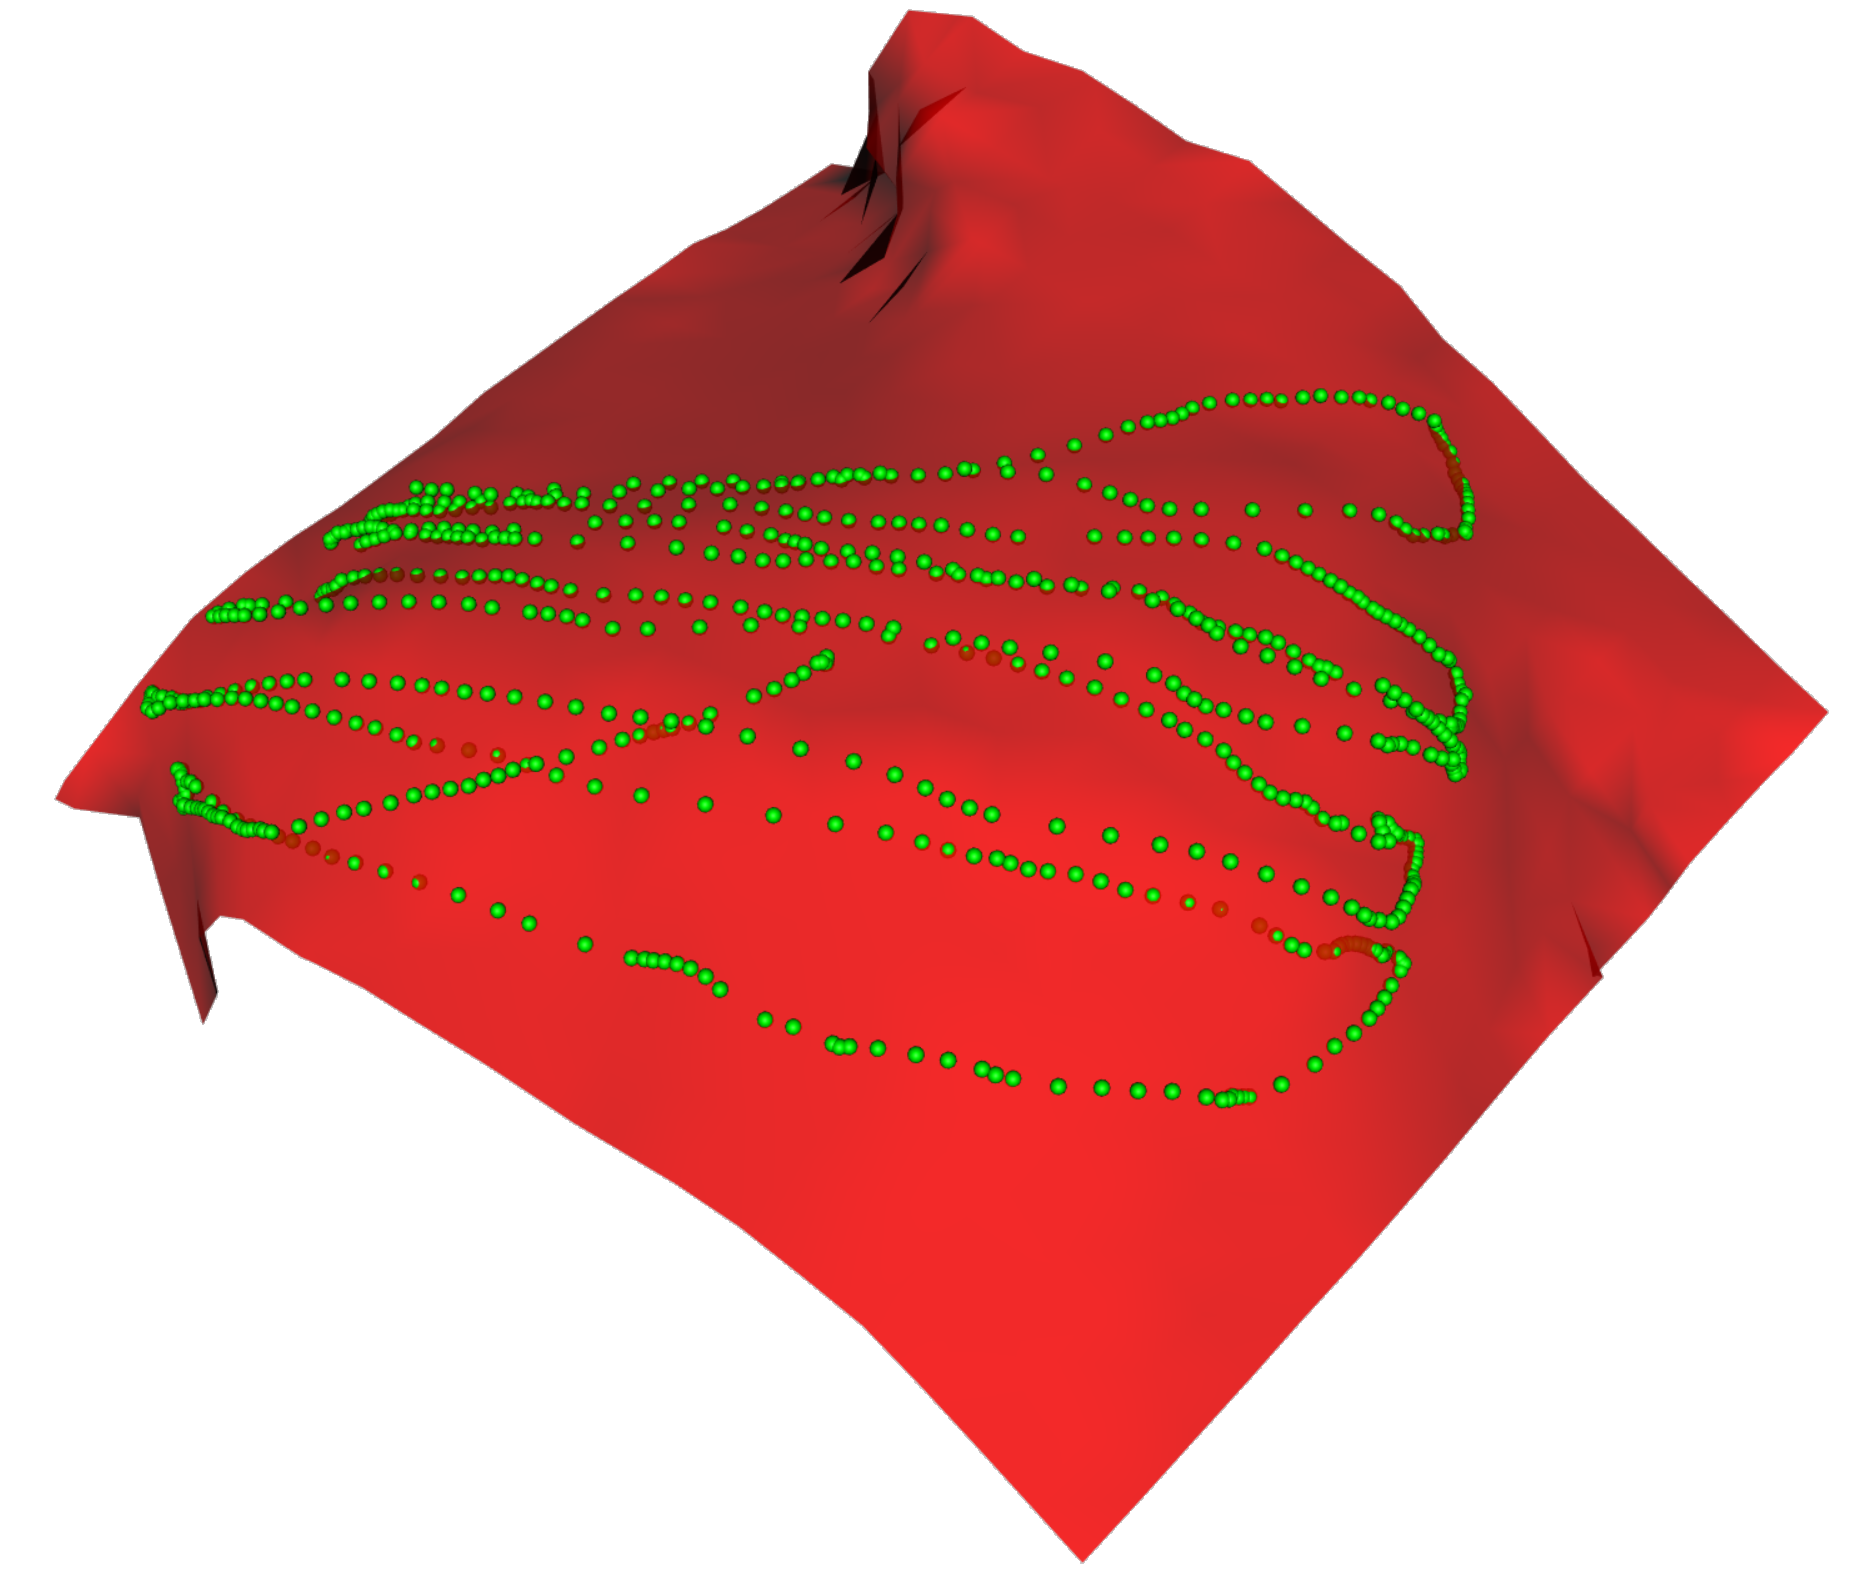
\includegraphics[width=0.3\linewidth]{mes11_sweepLR.png}}
    \\
    \small Spiral out & Spiral in & Sweep LR
    \\
    \hline
    \addheight{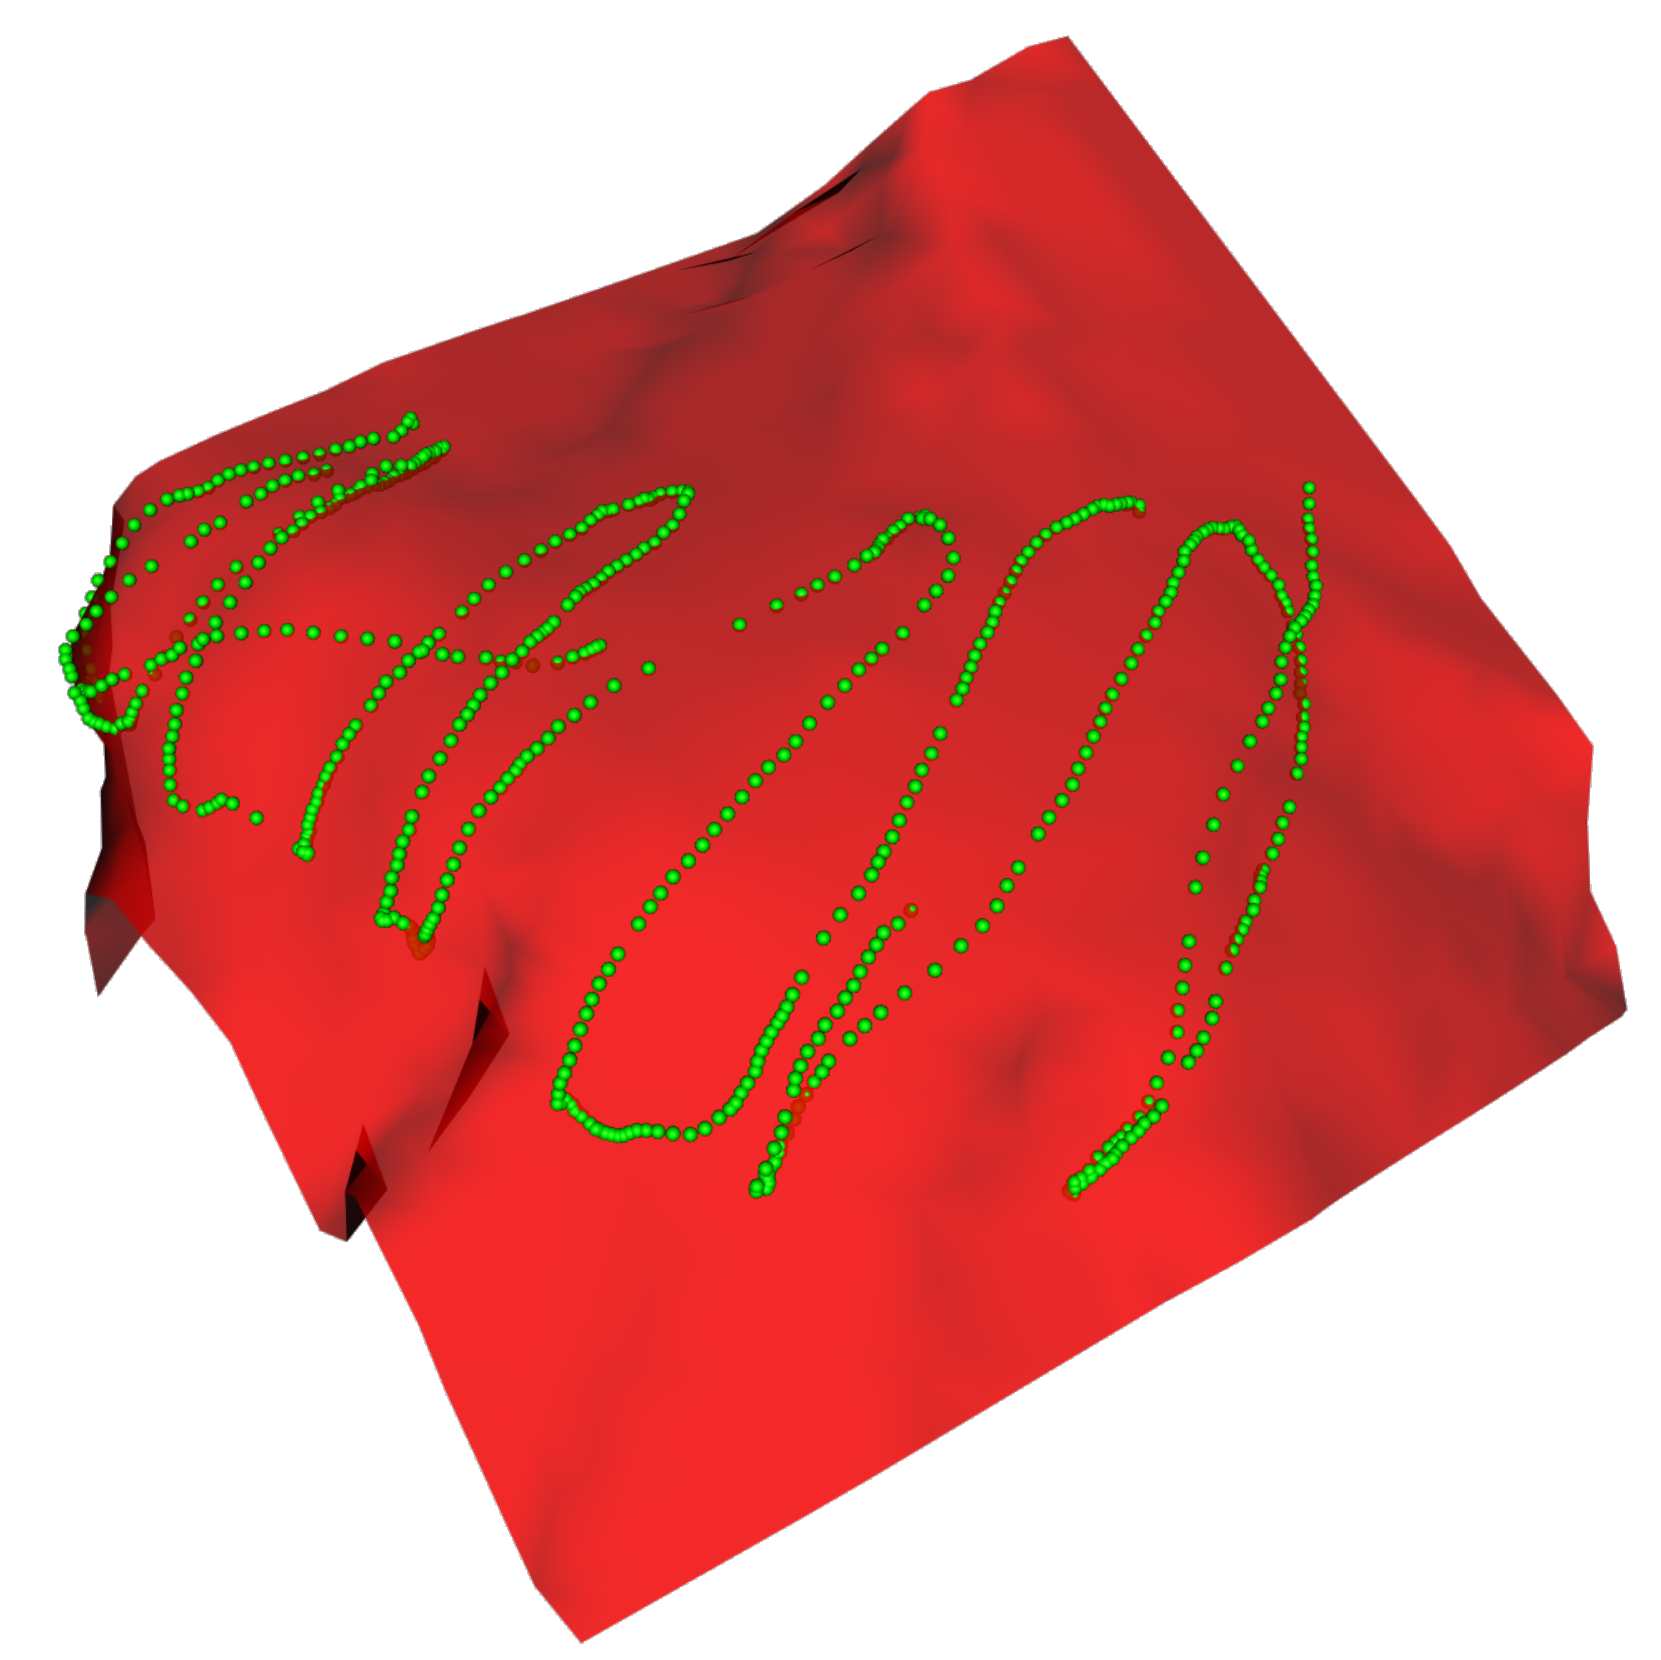
\includegraphics[width=0.3\linewidth]{mes12_sweepFB.png}} &
    \addheight{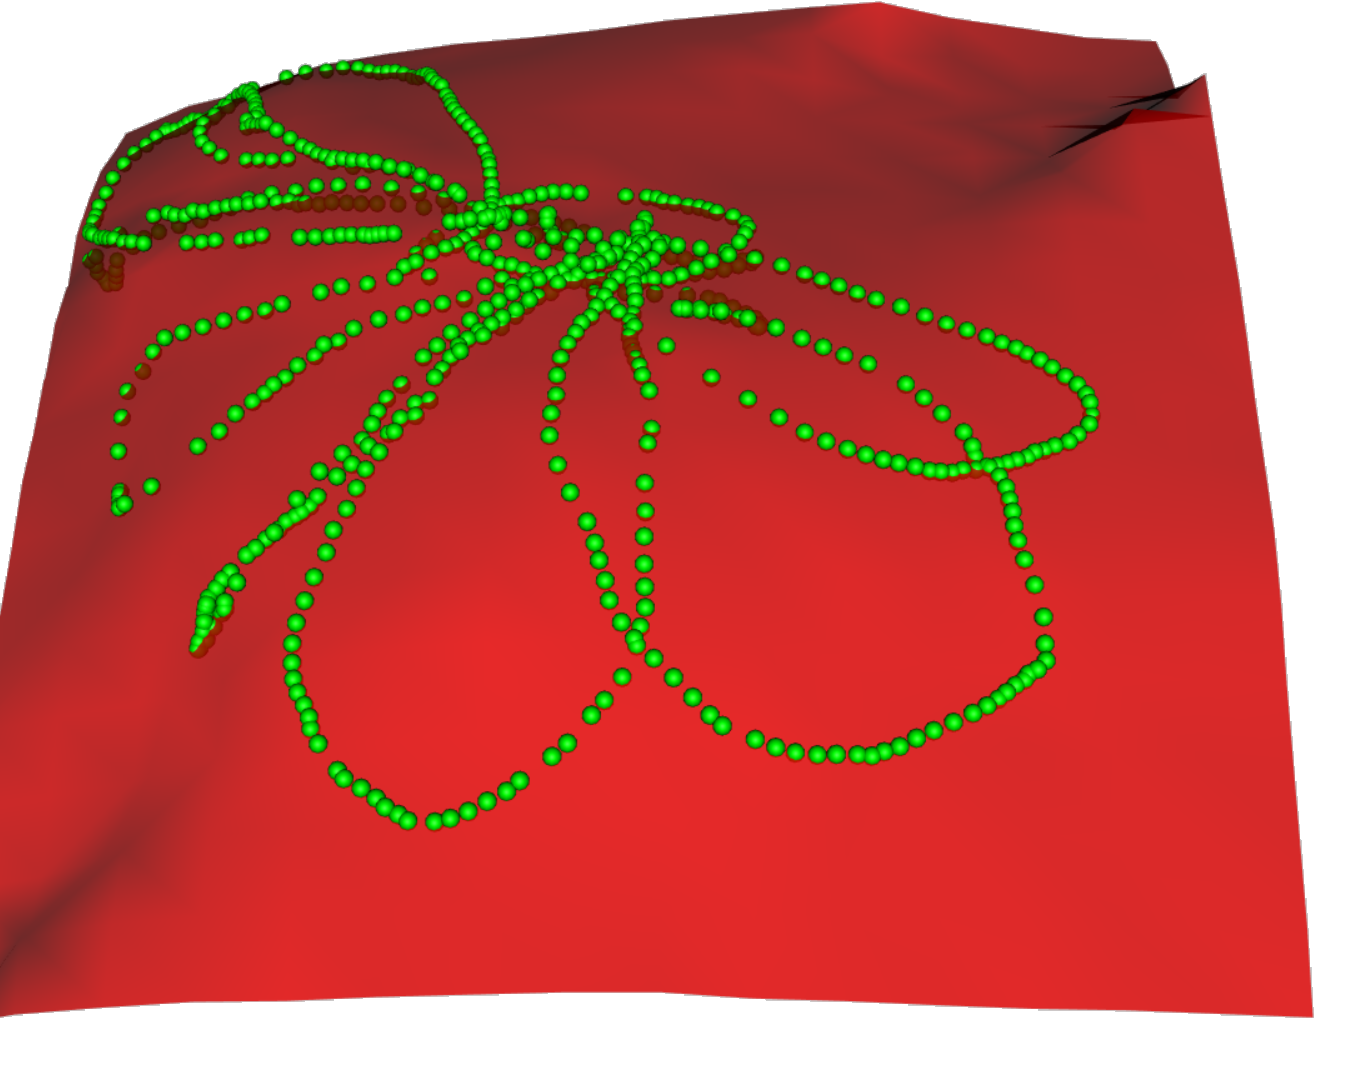
\includegraphics[width=0.3\linewidth]{mes07_flower.png}} &
    \addheight{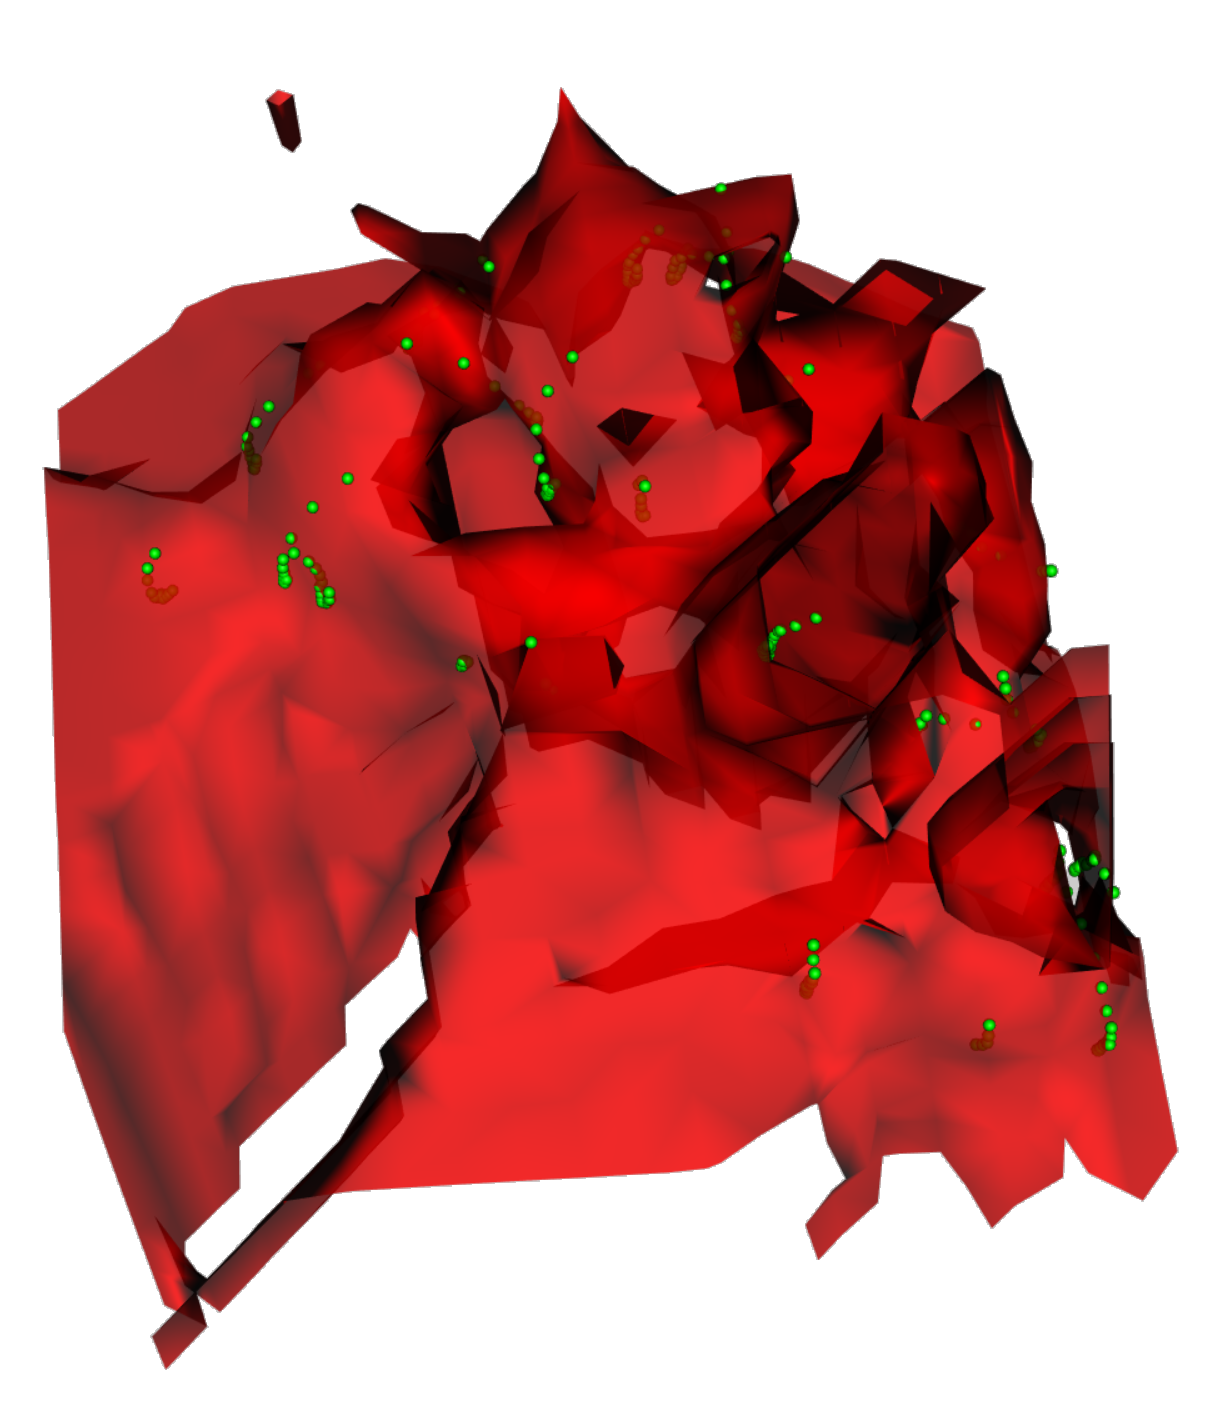
\includegraphics[width=0.3\linewidth]{mes08_pointgrid.png}}
    \\
    \small Sweep FB & Flower & Point grid
    \\
  \end{tabular}
  \caption{Reconstructed surfaces from different movements of the ultrasound device over the
    surface of the liver model. The names correspond to the movement drawings in figure \ref{fig:movements}}
  \label{fig:soft_liver_movements}
\end{figure}
\textbf{Quantitative analysis}

To evaluate the accuracy of the reconstructed surfaces, the shortest distance of
the reference points to the surface were computed. The overall median error for all the measurements is 2,5mm with an
interquartile range of 1 mm – 5 mm. By projecting these errors corresponding to
each reference point onto the liver surface, one can see that the highest errors
are in segments 2 and 3 And the lowest in segments 4, 5, 6 and 8 (Figure \ref{fig:surfaceErrors}).

\begin{figure}[H]
  \centering
 \includegraphics[width=\textwidth]{surfaceErrors}
 \caption{The mean distance of each reference point visualized by colors. All
   points with a mean distance of over 5 mm to the surface are colored dark red.
   Points with a mean distacne below 1.5 mm are colored dark green.}
  \label{fig:surfaceErrors}
\end{figure}

\subsection{Discussion}
The surface contact detector is correctly classifying in 96\% of the cases, with
a very low false positive rate of 1.9\%. This is especially important, as false
positives lead to artifacts in the reconstructed surface. Furthermore, the
processing time of 15 ms per image makes it suitable for real-time processing of
the images as the ultrasound scanner runs at 20 Hz (50 ms / frame). When the US
probe is removed from the liver surface there are 3-5 images which are wrongly
classified as having a signal. This would cause artifacts in the surface
reconstruction, and therefore they are filtered out later for surface
reconstruction. This is mainly, because of the latency of the US scanner itself
compared to the tracking system. The images are slightly blurrier (Figure \ref{fig:classificationProblem}), but
from the tracking positions one can clearly see that they are not on the
surface.

% \begin{figure}[H]
%   \centering
%  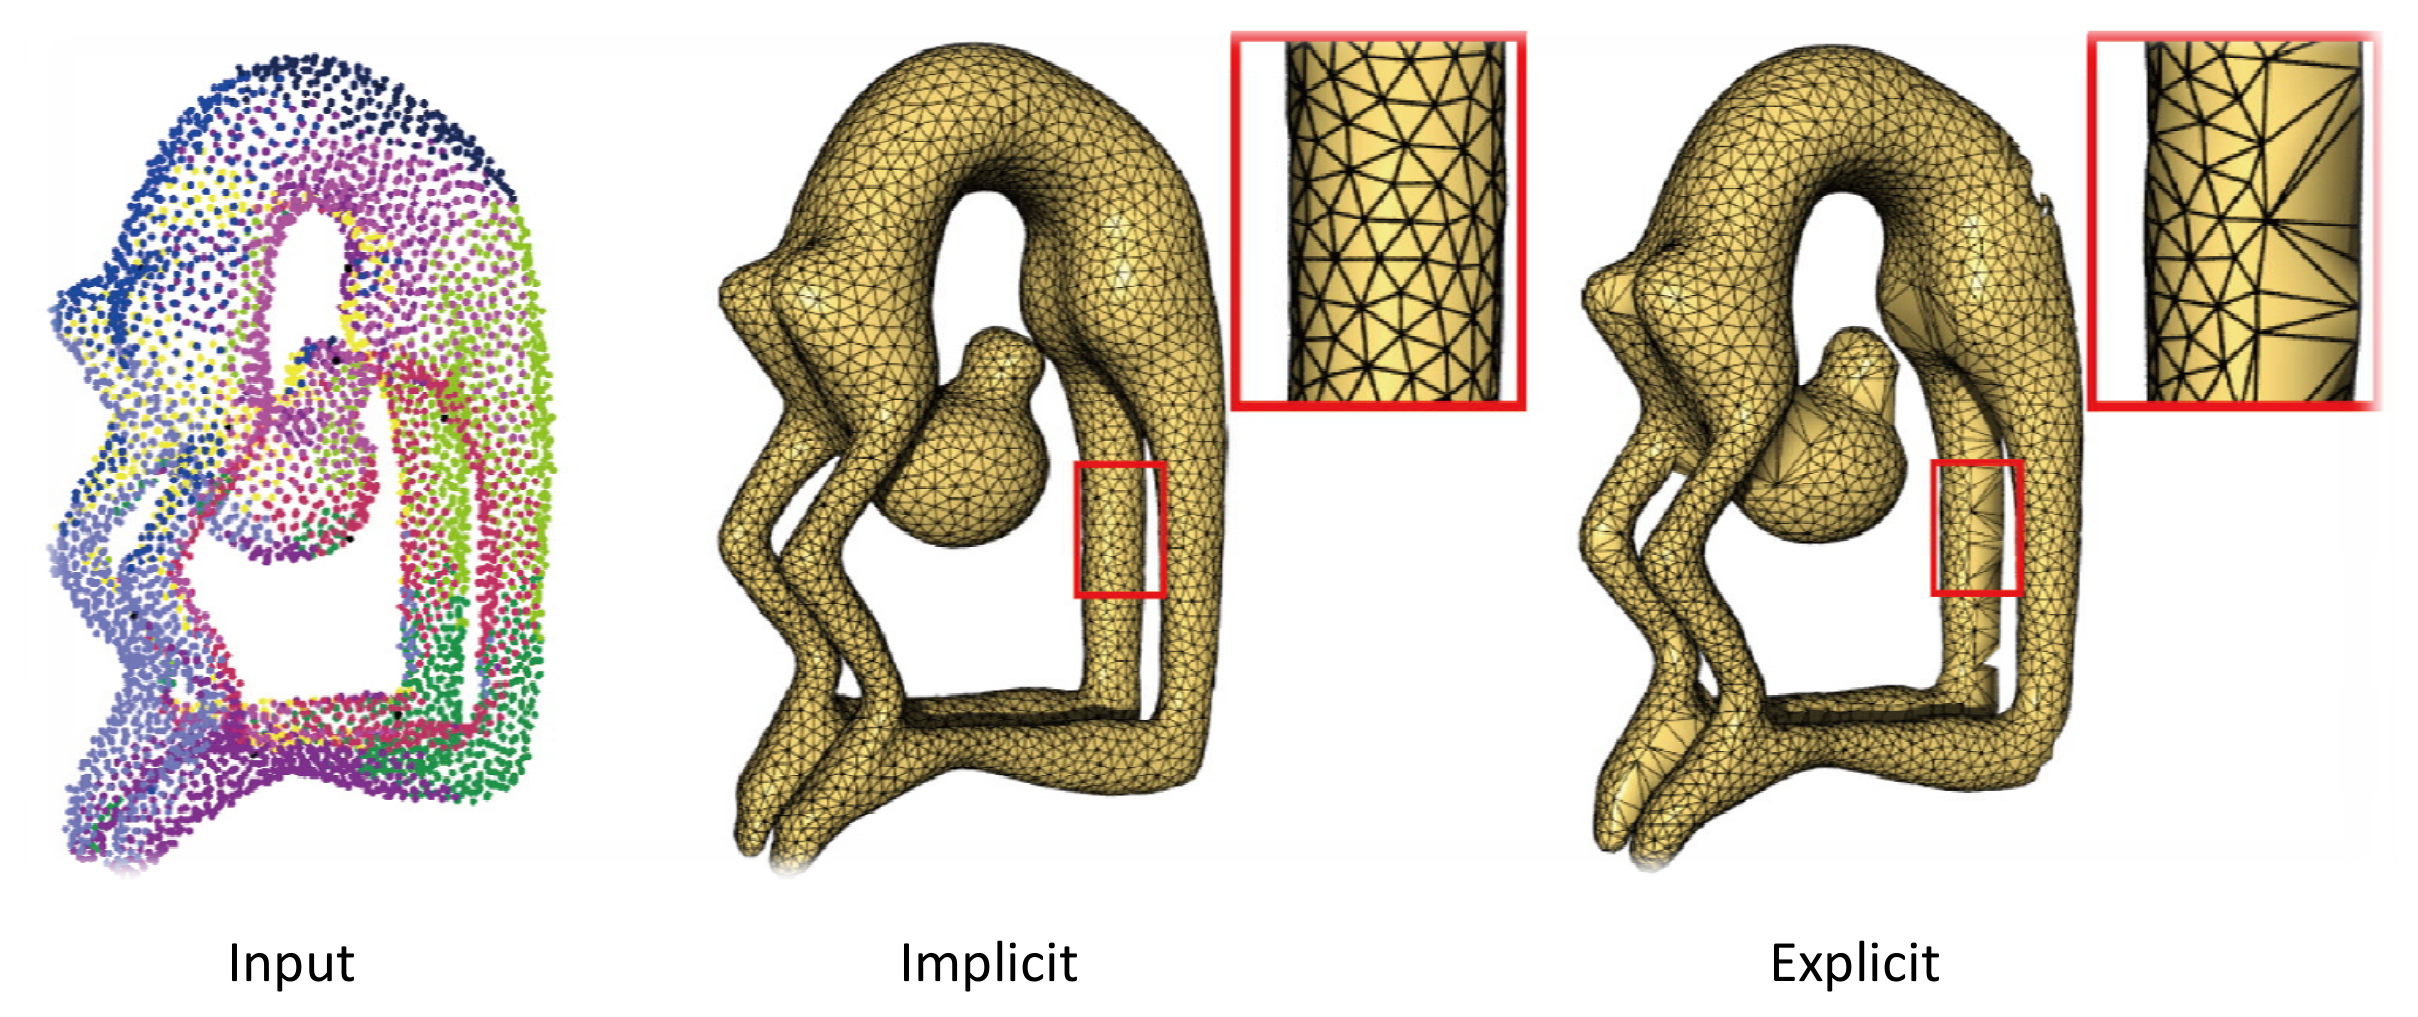
\includegraphics[width=\textwidth]{ImplicitVSExplicit}
%  \caption{Wrong and correct classified images at the end of the measurement}
%   \label{fig:ImplicitVSExplicit}
% \end{figure}

\begin{figure}[H]
  \centering
  \minipage{0.32\linewidth}
    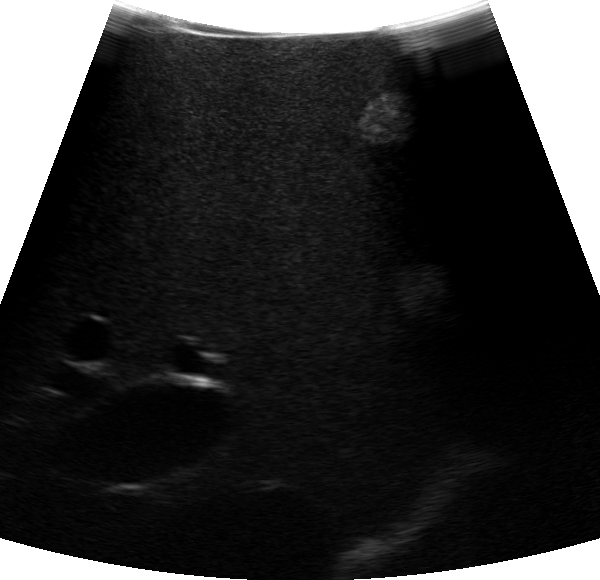
\includegraphics[width=\linewidth]{wrong_classified}
  \endminipage
  \minipage{0.1\linewidth}
  \hfill
  \endminipage
  \minipage{0.32\linewidth}
    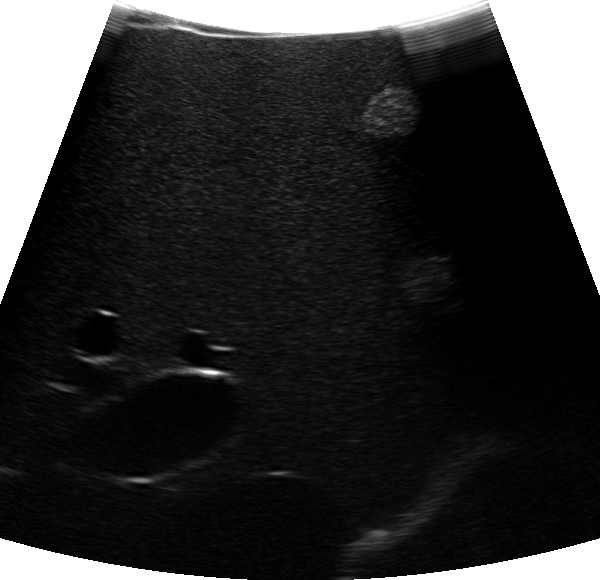
\includegraphics[width=\linewidth]{correct_classified}
  \endminipage
  \caption{Wrong and correct classified images at the end of the measurement}
  \label{fig:classificationProblem}
\end{figure}

\subsubsection{Surface reconstruction}
From a visual point of view the reconstructed surfaces of the US liver phantom
look similar to the surface of the liver model. However, the spiral and the
flower movement, led to a more accurate reconstruction.

From a quantitative point of view, it turned out that the largest average errors
are in segment 2 and 3. This is likely because these liver segments are the
softest on the phantom used for the measurements. Due to that, this segment was
pressed down during the measurement which lead to a surface with a large
distance to the reference points. Additionally, one can see that the average
distance at the boundary of the liver is large as well. This could be because
the US device was held between the wall of the tank and the liver model. Because
of the small space between the wall and the liver, the pressure applied on the
liver was larger than in other areas and the consequent distance between the
reference points and the deformed surface became larger. However, this might
also be the case in a clinical setting, as these regions are more difficult to
reach with the US probe. Overall, the best accuracy, could be achieved in
segments 4,5,6 and 8, which were the easiest to access in this setup. In a next
step, this would also be analyzed on the human liver, to see in which segments
this technique can be applied accurately.

To conclude, we presented a surface reconstruction technique, which can be used
to intraoperatively acquire a surface model of the liver using navigated US.
This can then be further used for intraoperative resection planning or
surface-based registration.


\section{Surface reconstruction on retrospective data}
\subsection{Methodology}
Retrospective data from Banz et. al
\subsection{Results}
\subsection{Discussion}

\section{Usability Test}
3 surgeons
questionnaire
surface accuracy (using surface registration)
\subsection{Methodology}
\subsection{Results}
\subsection{Discussion}
%%% Local Variables:
%%% TeX-master: "MscThesis"
%%% End:
%%%%%%%%%%%%%%%%%%%%%%%%%%%%%%%%%%%%%%%%%%%%%%%%%%%%%%%%%%%%%%%%%%%%%%%%
% This is the conclusion chapter file.
%%%%%%%%%%%%%%%%%%%%%%%%%%%%%%%%%%%%%%%%%%%%%%%%%%%%%%%%%%%%%%%%%%%%%%%%
%
% Author:   René Widmer
%           Institute for Surgical Technology and Biomechanics ISTB
%           University of Bern
%           rene.widmer@istb.unibe.ch
%
% Date:     10/28/2009
%
%%%%%%%%%%%%%%%%%%%%%%%%%%%%%%%%%%%%%%%%%%%%%%%%%%%%%%%%%%%%%%%%%%%%%%%%

\chapter{Discussion and Conclusions}

\section{Discussion}

\textit{Interpret your results in the context of past and current studies and literature on the same topic. Attempt to explain inconsistencies or contrasting opinion. Highlight the novelty of your work. Objectively discuss the limitations.}

\section{Conclusions}

\textit{Formulate clear conclusions which are supported by your research results.}

\endinput
%%% Local Variables:
%%% TeX-master: "MscThesis"
%%% End:
%%%%%%%%%%%%%%%%%%%%%%%%%%%%%%%%%%%%%%%%%%%%%%%%%%%%%%%%%%%%%%%%%%%%%%%%
% This is the outlook chapter file.
%%%%%%%%%%%%%%%%%%%%%%%%%%%%%%%%%%%%%%%%%%%%%%%%%%%%%%%%%%%%%%%%%%%%%%%%
%
% Author:   René Widmer
%           Institute for Surgical Technology and Biomechanics ISTB
%           University of Bern
%           rene.widmer@istb.unibe.ch
%
% Date:     10/28/2009
%
%%%%%%%%%%%%%%%%%%%%%%%%%%%%%%%%%%%%%%%%%%%%%%%%%%%%%%%%%%%%%%%%%%%%%%%%

\chapter{Outlook}

\textit{Provide a vision of possible future work to continue and extend your thesis research.}

\endinput

% Uncomment this if you'd like to suppress the numbering of the
% appendices.
%\backmatter

%%%%%%%%%%%%%%%%%%%%%%%%%%%%%%%%%%%%%%%%%%%%%%%%%%%%%%%%%%%%%%%%%%%%%
% Bibliography
%%%%%%%%%%%%%%%%%%%%%%%%%%%%%%%%%%%%%%%%%%%%%%%%%%%%%%%%%%%%%%%%%%%%%
% Force every reference to show up (demo)
\nocite{*}
\bibliography{References}

{
   \vskip1em
   \noindent\textit{etc.}
} % Remove this block.

%%%%%%%%%%%%%%%%%%%%%%%%%%%%%%%%%%%%%%%%%%%%%%%%%%%%%%%%%%%%%%%%%%%%%
% Appendices
%%%%%%%%%%%%%%%%%%%%%%%%%%%%%%%%%%%%%%%%%%%%%%%%%%%%%%%%%%%%%%%%%%%%%
\part*{Appendices}
\begin{appendix}
	%%%%%%%%%%%%%%%%%%%%%%%%%%%%%%%%%%%%%%%%%%%%%%%%%%%%%%%%%%%%%%%%%%%%%%%%
% This file contains the description of tensor mathematics used during
% the thesis.
%%%%%%%%%%%%%%%%%%%%%%%%%%%%%%%%%%%%%%%%%%%%%%%%%%%%%%%%%%%%%%%%%%%%%%%%
%
% Author:	Ren� Widmer
%
% Date:		11/29/2008
%
%%%%%%%%%%%%%%%%%%%%%%%%%%%%%%%%%%%%%%%%%%%%%%%%%%%%%%%%%%%%%%%%%%%%%%%%

\chapter{Questionnaires}
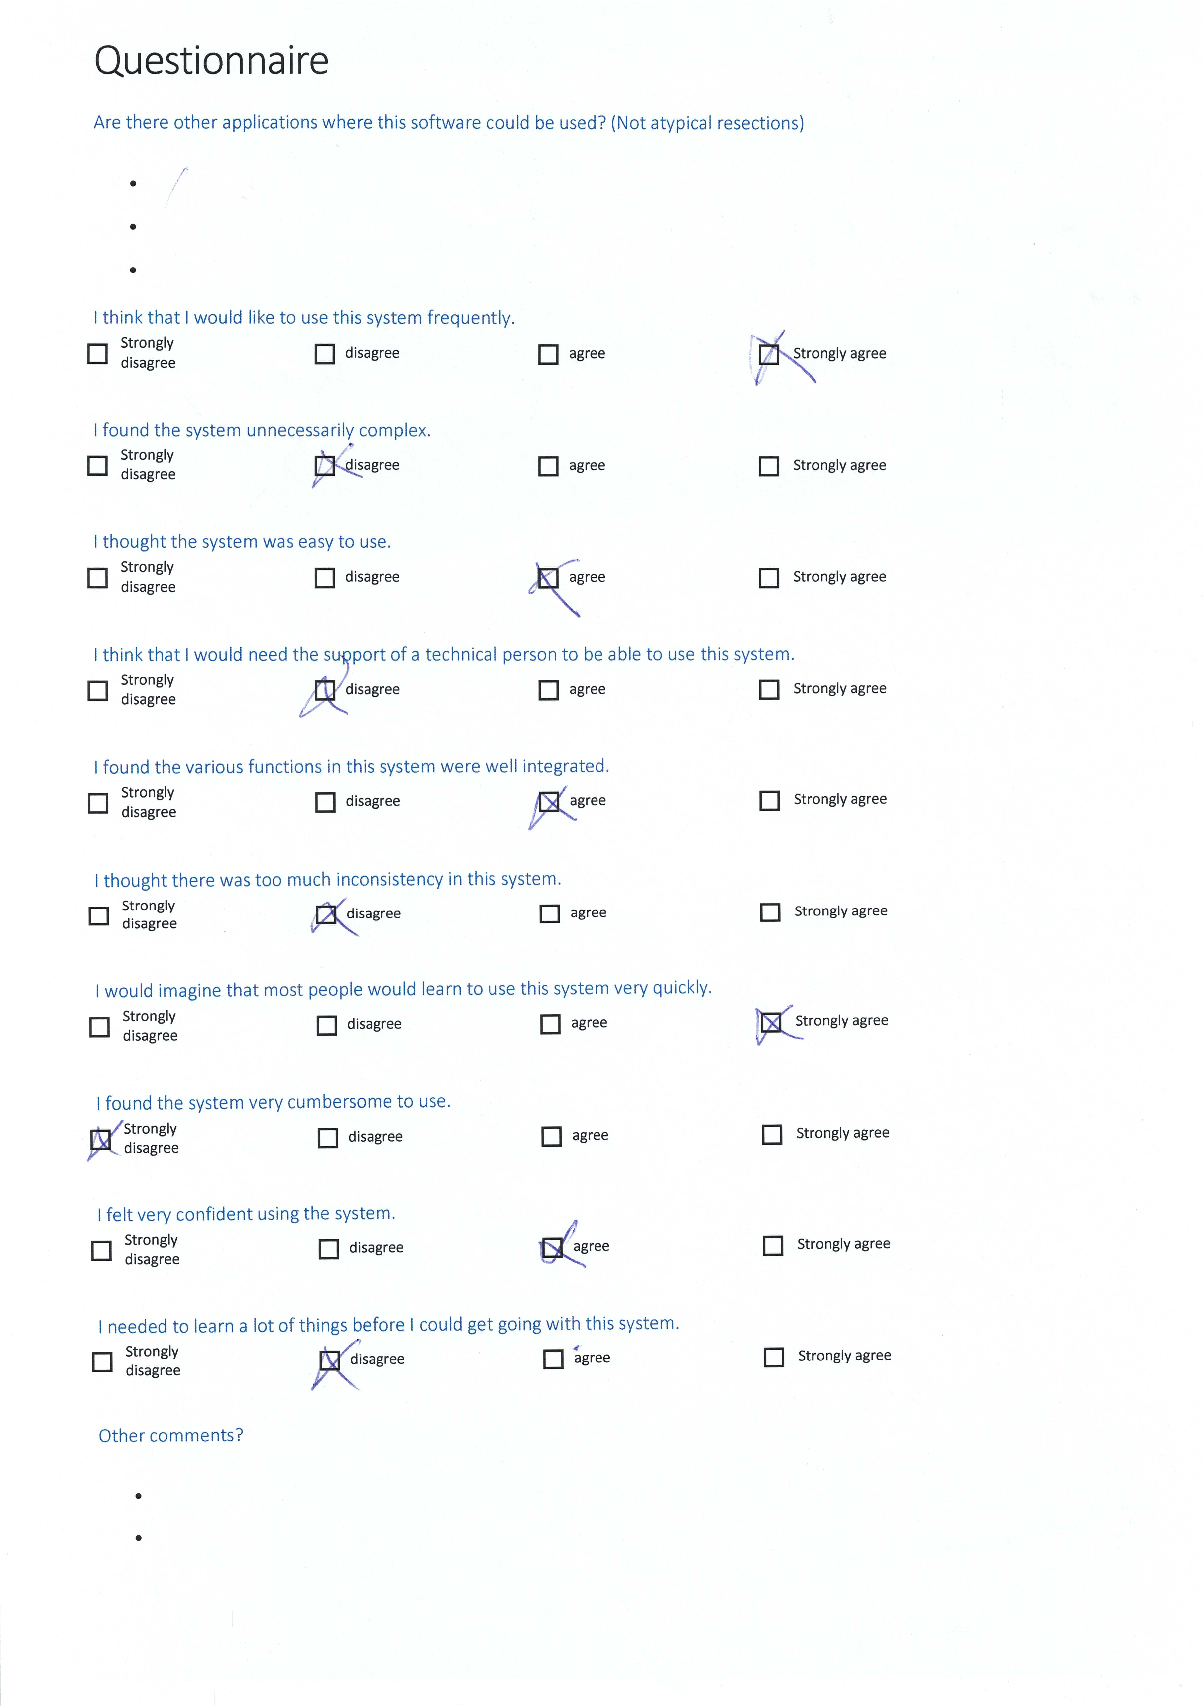
\includepdf[pages=-,scale=.7,pagecommand={},linktodoc=true]{Questionnaire1.pdf}
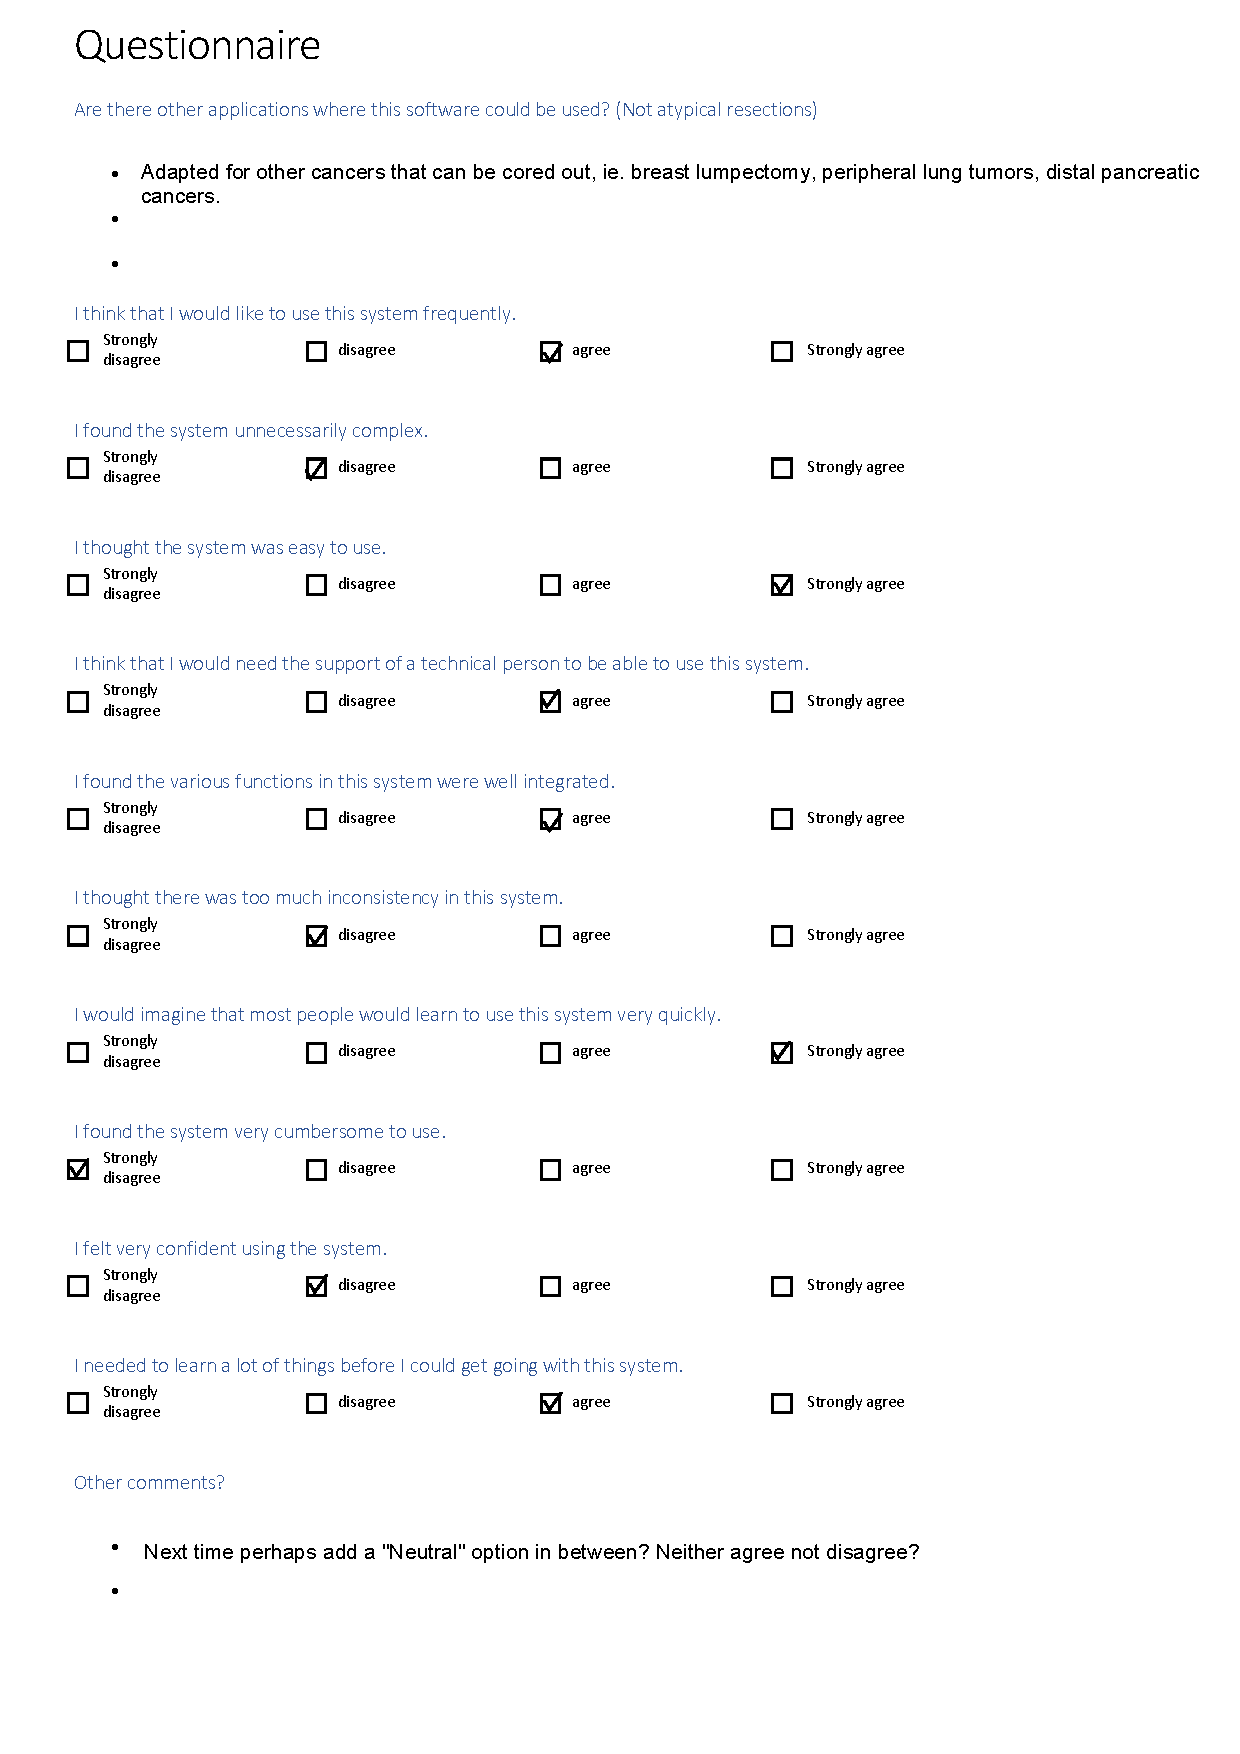
\includepdf[pages=-,scale=.7,pagecommand={},linktodoc=true]{Questionnaire2.pdf}
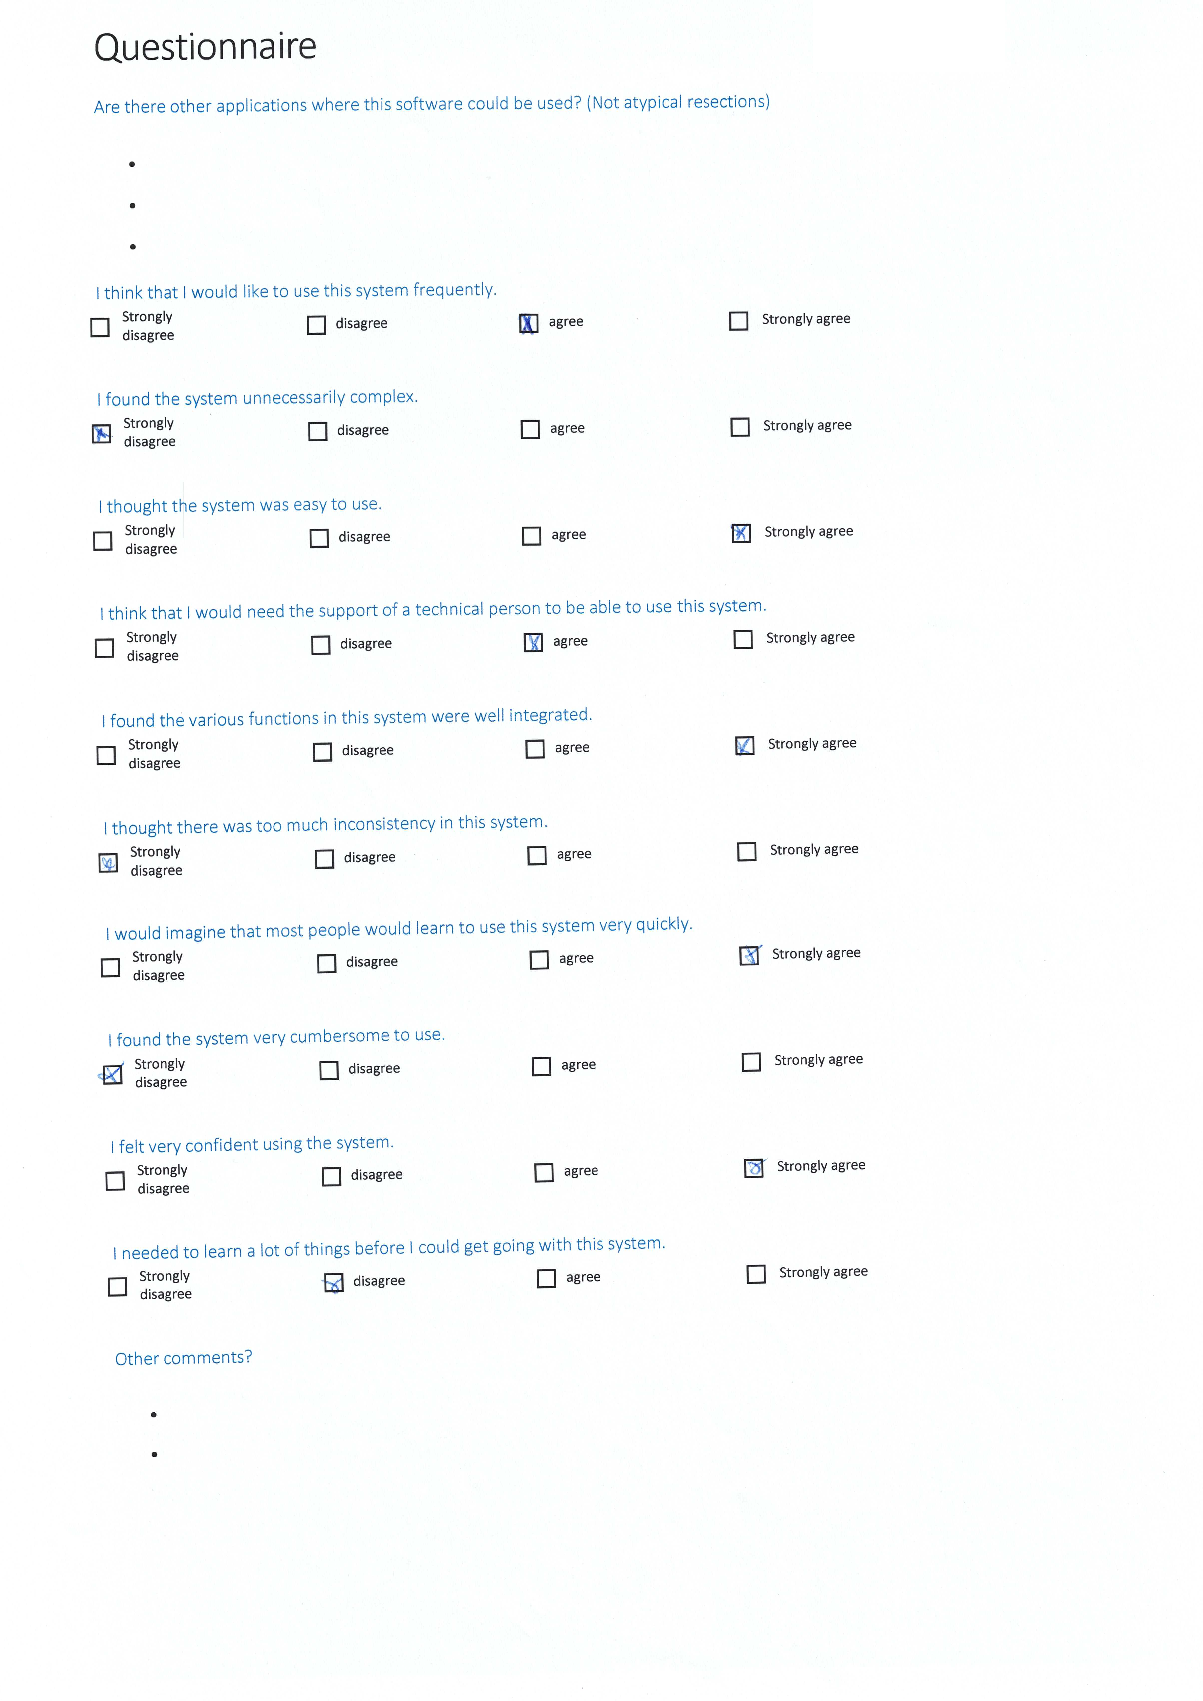
\includepdf[pages=-,scale=.7,pagecommand={},linktodoc=true]{Questionnaire3.pdf}
%%% Local Variables:
%%% TeX-master: "MscThesis"
%%% End:
	\chapter{Another Appendix}

\section{Section 1}

...

\section{Section 2}

...
%%% Local Variables:
%%% TeX-master: "MscThesis"
%%% End:
\end{appendix}

\end{document}

\endinput
%%% Local Variables:
%%% TeX-master: t
%%% End: